% book example for classicthesis.sty
\documentclass[
  % Replace twoside with oneside if you are printing your thesis on a single side
  % of the paper, or for viewing on screen.
  english,
  oneside,
  11pt, a4paper,
  footinclude=true,
  headinclude=true,
  cleardoublepage=empty
]{scrbook}

\usepackage[linedheaders,parts,pdfspacing]{classicthesis}

\usepackage{amsmath}
\usepackage{amsthm}
\usepackage{acronym}
\usepackage[nottoc,numbib]{tocbibind}

\usepackage{geometry}
\geometry{margin=1in}
\linespread{1.3}

% New Lines not Indentation for Paragraphs
\usepackage[parfill]{parskip}

\usepackage{hyperref}

% Styling Contents Page
\usepackage{tocstyle} 
\newtocstyle[classic][]{newstyle}{%
  \settocfeature[0]{entryhook}{\bfseries}%
  \settocfeature[0]{entryvskip}{0.8em plus 20pt}%
}
\usetocstyle{newstyle}

% Style Headings
\usepackage{titlesec}
\usepackage{indentfirst}
\newlength{\normalparindent}
\AtBeginDocument{\setlength{\normalparindent}{\parindent}}

\titleformat{\chapter}[display]
   	% Format
   	{\huge}
   	% Label
   	{}
   	%Separation
   	{-40pt}
   	% Before
    {
    	\titlerule\vspace*{0.4\baselineskip}
    	\ifnum\thechapter=0 \hspace*{0.5em} \else \thechapter. \fi
    	\spacedallcaps
    }
    % After
    [\normalcolor\normalsize\vspace*{.8\baselineskip}\titlerule]
\titlespacing\chapter{0pt}{0pt}{10pt}[0pt]
  
\titleformat{\section}[display]
   	% Format
   	{\large\bfseries}
   	% Label
   	{}
   	%Separation
   	{-2em}
   	% Before
    {
    	\thesection \hspace*{0.25em} - \spacedallcaps
    }
    % After
    []
\titlespacing\section{0pt}{0pt}{0pt}

\titleformat{\subsection}[display]
   	% Format
   	{\small\bfseries}
   	% Label
   	{}
   	%Separation
   	{-2em}
   	% Before
    {
    	\hspace*{1em} \spacedallcaps
    }
    % After
    []
\titlespacing\subsection{0pt}{0pt}{0pt}

% Shiny Pictures
\usepackage{float}
\usepackage{graphicx}
\usepackage{caption}
\usepackage{subcaption}
\usepackage{wrapfig}

% Font
\usepackage{fontspec}
\setmainfont{Quicksand}
%\usepackage{unicode-math}
%\setmathfont{Quicksand}
%\setsansfont{TeX Gyre Heros}[Scale=MatchLowercase]
%\setmonofont{Inconsolata}[Scale=MatchLowercase]

% Date
\usepackage{babel}
\usepackage[]{datetime}

\usepackage{textcase}

% Frame
\include{xcolor}

% Section References
\newcommand\sectionreference[1]{\begin{flushleft}\small\textit{#1}\end{flushleft}}

\include{ragged2e}

\begin{document}

\makeatletter
\patchcmd{\l@subsection}{#1}{\MakeTextUppercase{#1}}{}{}
\makeatother

\begin{titlepage}

\newcommand{\HRule}{\rule{\linewidth}{0.3mm}} % Defines a new command for the horizontal lines, change thickness here

%----------------------------------------------------------------------------------------
%	LOGO SECTION
%----------------------------------------------------------------------------------------

\begin{figure}
  \begin{flushleft}% or better \raggedleft see comments below
	
\includegraphics[height=1.5cm]{logo.eps}\\[2cm] % Include a department/university logo - this will require the graphicx package
  \end{flushleft}
\end{figure}

\center % Center everything on the page
 
%----------------------------------------------------------------------------------------
%	HEADING SECTIONS
%----------------------------------------------------------------------------------------

% \textsc{\LARGE Imperial College London}\\[0.5cm] % Name of your university/college
\textsc{\Large Department of Computing}\\[0.5cm] % Major heading such as course name
% \textsc{\large Minor Heading}\\[0.5cm] % Minor heading such as course title

%----------------------------------------------------------------------------------------
%	TITLE SECTION
%----------------------------------------------------------------------------------------

\HRule \\[0.4cm]
{ \LARGE \bfseries Visualizing uncertainty in super-resolution fetal MRI.}\\[0cm] % Title of your document
\HRule \\[1.5cm]
 
%----------------------------------------------------------------------------------------
%	AUTHOR SECTION
%----------------------------------------------------------------------------------------

\begin{minipage}{0.4\textwidth}
\begin{flushleft} \large
\emph{Author:}\\
Sam Esgate % Your name
\end{flushleft}
\end{minipage}
~
\begin{minipage}{0.4\textwidth}
\begin{flushright} \large
\emph{Supervisor:} \\
Dr. Bernhard Kainz % Supervisor's Name
\end{flushright}
\end{minipage}\\[7cm]

% If you don't want a supervisor, uncomment the two lines below and remove the section above
%\Large \emph{Author:}\\
%John \textsc{Smith}\\[3cm] % Your name

%----------------------------------------------------------------------------------------
%	DATE SECTION
%----------------------------------------------------------------------------------------

{\large \today}\\[3cm] % Date, change the \today to a set date if you want to be precise
 
%----------------------------------------------------------------------------------------

\vfill % Fill the rest of the page with whitespace

\end{titlepage}

% The abstract is a very brief summary of the report's contents. 
% It should be about half a page long. 
% Somebody unfamiliar with your project should have a good idea of what it's about having read the abstract alone and will know whether it will be of interest to them. 
% Note that the abstract is a summary of the entire project including its conclusions. 
% A common mistake is to provide only introductory elements in the abstract without saying what has been achieved.

\chapter*{Abstract}

Some abstract thoughts... do this last.

% It is usual to thank those individuals who have provided particularly useful assistance, technical or otherwise, during your project. 
% Your supervisor will obviously be pleased to be acknowledged as he or she will have invested quite a lot of time overseeing your progress.
\chapter*{Acknowledgements}

Special thanks to \textbf{Bernhard Kainz} whose guidance was invaluable.

Thanks also to everybody who gave their time to help with the evaluation:

\begin{itemize}
	\item Amir Alansary
	\item Paul Aljabar
	\item Joshua van Amerom
	\item Rose Crowley
	\item Alice Davidson
	\item Matt Fox
	\item Kevin Keraudren
	\item Maelene Lohezic
	\item Kerstin Pannek
	\item Prachi Patkee
\end{itemize}

% This should list the main chapters and (sub)sections of your report. 
% Choose self-explanatory chapter and section titles and use double spacing for clarity.
% If possible you should include page numbers indicating where each chapter/section begins.
% Try to avoid too many levels of subheading - three is sufficient.

%*******************************************************
% Table of Contents
%*******************************************************
\pdfbookmark[1]{\contentsname}{tableofcontents}

\setcounter{tocdepth}{3} % <-- 2 includes up to subsections in the ToC
\setcounter{secnumdepth}{3} % <-- 3 numbers up to subsubsections

\tableofcontents 

%*******************************************************
% List of Figures and of the Tables
%*******************************************************
\iffalse
%*******************************************************
% List of Figures
%*******************************************************    
\pdfbookmark[1]{\listfigurename}{lof}
\listoffigures

%*******************************************************
% List of Tables
%*******************************************************
\pdfbookmark[1]{\listtablename}{lot}
\listoftables
  
%*******************************************************
% List of Listings
%******************************************************* 
\pdfbookmark[1]{\lstlistlistingname}{lol}
\lstlistoflistings 
   
%*******************************************************
% Acronyms
%*******************************************************
\pdfbookmark[1]{Acronyms}{acronyms}
\chapter*{Acronyms}
\begin{acronym}[UML]
    \acro{DRY}{Don't Repeat Yourself}
    \acro{API}{Application Programming Interface}
    \acro{UML}{Unified Modeling Language}
\end{acronym} 
\fi


\chapter{Introduction}\label{chapter:introduction}

% Provide necessary background.
% Why is the project important?

Magnetic Resonance Imaging (MRI) has found itself being used in an ever increasing number of applications. Uses range from imaging the spinal cord and heart to detecting brain activity (fMRI) and refinements to the technique have resulted in its use in fetal imaging increasing.

In many ways MRI is highly suited to fetal imaging; it has impressive contrast in soft tissue and no known harmful side effects. However, limitations in resolution make imaging what can often be very small area difficult. Super resolution reconstruction is a technique designed to mitigate this problem by constructing a high resolution volume from a number of lower resolution scans.

Of course the quality of the reconstruction depends on the quality of these scans. If, for example, the fetus moves during the scanning process, then some areas will be less well sampled than others. This results in less data to use in some areas of the reconstruction than others and gives rise to areas of high uncertainty.
 
From just looking at the reconstructed image it is not necessarily obvious where these areas are. Crucially when using these images for diagnostic purposes it very is important to be aware of this. If a diagnosis needs to be made based on a region of the reconstruction with high uncertainty then this indicates that further scanning may be required.

% Specify main objectives.
% Specify main contributions - provide section numbers.

The main aim of the project was to prototype visualizations that can communicate the uncertainty of a reconstruction to researchers and radiographers. This will allow them to both gauge how well a reconstruction went and highlight any particular problem areas.

Two distinctive approaches have been prototyped and their effectiveness has been evaluated with a group of expert users. The first technique (section \ref{section:thresholding}) uses thresholding to show areas of the scan within a particular uncertainty range; the areas that fall in a given range (e.g. the worst 1$\%$) can then be displayed on top of the scan in 2D and as a volume in 3D. The second technique (section \ref{section:uncertaintysurface}) projects the uncertainty in a scan on to a surface representation of the object that has been scanned, highlighting the worst regions.

These trade-offs off the two approaches have been looked at to see what works well and where future development should be focused. See chapter \ref{chapter:evaluation}.

As well as being able to visualize the uncertainty, recent research\cite{uncertaintysvd} has shown that it is possible to use the uncertainty to guide the scanning process. The idea is if we can compute, at the time of scanning, the areas of high uncertainty then we can then tailor the next scan position and direction to target these problem areas. A visualization designed to communicate this information has also been created (see section \ref{section:nextscanplane}) and also evaluated.

\subsection{TODO}
The prototype that has been developed also forms the basis of a research tool to combine the... bla bla bla... pipeline... was the Research Tool an objective?
% Specify objectives that didn't get met.

TODO: What objectives weren't accomplished?
\begin{enumerate}
	\item Registering a generic model to a volume.
	\item Animation.	
\end{enumerate}

Hopefully the findings of this project will be able to guide the incorporation of these techniques in clinical use.

% Why is the project difficult - discuss problems to overcome?

\chapter{Background}

% ------------------------- %
% ---- MEDICAL IMAGING ---- %
% ------------------------- %
\section{Medical Imaging}\label{background:medicalimaging}
The field of medical imaging came into existence with the discovery of x-rays in 1895 by Wilhelm R\"{o}ntgen\cite{rontgen}. This meant that for the first time it was possible to peek into the human anatomy without having to physically open it up. This revolution came at a cost however as at the time the dangers of high doses of radiation were not understood and many of the pioneers died as a result of exposure\cite{xraydeath}.

Radiology, the use of ionizing radiation to image objects, was greatly refined over the years; contrast agents were developed which made fields like angiography (imaging of blood vessels) possible\cite{infinityhistory} and the doses used were refined to dramatically decrease the associated risks. X-rays have been used successfully in medical imaging ever since and in the 70s the invention of the CT (X-Ray Computed Tomography) scanner allowed them to be used to produce 3D images of the body.

It was not until the 1980s that magnetic resonance imaging (MRI) was first used for medical diagnosis. MRI is based on the principles of nuclear magnetic resonance (NMR), which had been used in chemical analysis since the 40s\cite{bshr:mallard}.

MRI can be used to create anatomical images by examining the varying water content in different parts of the body. More recently MRI has been used to create functional images of the brain by using the same principals to detect blood flow\cite{fmri}. Unlike CT, which uses x-rays, MRI does not require the use of any ionizing radiation to perform the scan.

As with all medical imaging techniques the benefits and risks need to be weighed up before a scan is performed. When imaging fetuses the risks are higher than normal and so in general CT scans tend not to be used wherever possible. MRI however, like US (ultrasound), is not associated with known adverse fetal effects\cite{pregnancyimagingguidelines}.

% ------------------------- %
% ---------- MRI ---------- %
% ------------------------- %
\newpage
\section{MRI}\label{background:mri}
\sectionreference{\cite{howmriworks} gives a very good overview of how MRI works. A brief summary is given below.}

MRI uses a strong magnetic field and radio waves to produce images of the body. MRI can be used to produce 2D, 3D and even 4D images and has the advantage that it doesn’t use any ionizing radiation during the scanning process.

MRI is able to detect the amount of water that is contained in different types of tissue in the body by exploiting a property of protons called spin. Each water molecule in the body contains two hydrogen atoms and the nucleus of each is a single proton.

MRI applies a strong uniform magnetic field to the area being imaged which causes the spins of the protons to line up with the direction of the field. Some of the protons line up in the same direction, with low energy, and some line up opposing the magnetic field, which have high energy.

When a particular radio frequency is then applied some of the lower energy protons flip to become higher energy and oppose the magnetic field, when the radio waves are stopped these protons then flip back, emitting a radio wave that can be detected.

The resonant frequency of radio wave that is required to excite the protons depends on the strength of the magnetic field. This property allows an area to be scanned by applying a gradient magnetic field and varying the radio frequency.

There are a number of different variations of MRI. T1-weighted scans are best for visualizing fat, calcification, hemorrhage, thyroid, liver and bone marrow whereas T2-weighted scans accentuate water content.
There are also a number of different ways of acquiring the scan. SSFSE (Single Shot Fast Spin Echo) works by acquiring each slice of the image in sequence whereas 2DGRE (Gradient Echo) acquires all of the slices simultaneously.

If the contrast that can be achieved with MRI is insufficient for the imaging then a contrast agent, such as gadolinium, can be administered to enhance it.

\section{Fetal MRI}\label{background:fetalmri}

Since MRI, like US, is a non-invasive procedure that doesn’t use ionizing radiation it is ideal for use in fetal imaging\cite{fetalmri}. While US remains the most common imaging modality used during pregnancy MRI has a number of advantages; in particular it has better contrast in soft tissue which allows individual organs to be better differentiated. US however remains more widely available, easier to apply, easier to staff and the cheaper and so is unlikely to be replaced as the main fetal imaging tool in the near future.

There are no known side effects associated with using MRI, however it is currently recommended to wait until the 17th or 18th WG (week of gestation) before performing MRI. This is partly a precautionary measure but also before then the size of the fetus and amount of movement limits the usefulness of the scan\cite{fetalmri}.

% -------------------------- %
% ---- Super-Resolution ---- %
% -------------------------- %
\newpage
\section{Slice-to-Volume Reconstruction}\label{background:superresolution}
The main challenge with using MRI for fetal imaging is dealing with movement. One of the ways that this effect can be minimized is to acquire the scan in the shortest time possible and typically this is achieved by using a large slice thickness. A typical slice thickness when performing a scan on a fetal brain is 3mm, which when compared to the size of the brain, which may only be 50mm, limits the diagnostic potential.

One solution to this problem is to take many scans and use SVR (Slice-to-Volume Reconstruction) techniques to combine them. SVR (Slice-to-Volume Reconstruction) is a technique used to align a number of motion corrupted slice stacks. Individual slices are assumed to have been acquired fast enough so that the amount of movement within it is negligible, however the target may well move in between slices as they are being acquired over the course of a few minutes.

Figure \ref{fig:svroverview} shows the outline of the procedure used in \cite{gpureconstruction} and the key steps are outlined below.

\begin{figure}[H]
    \centering
	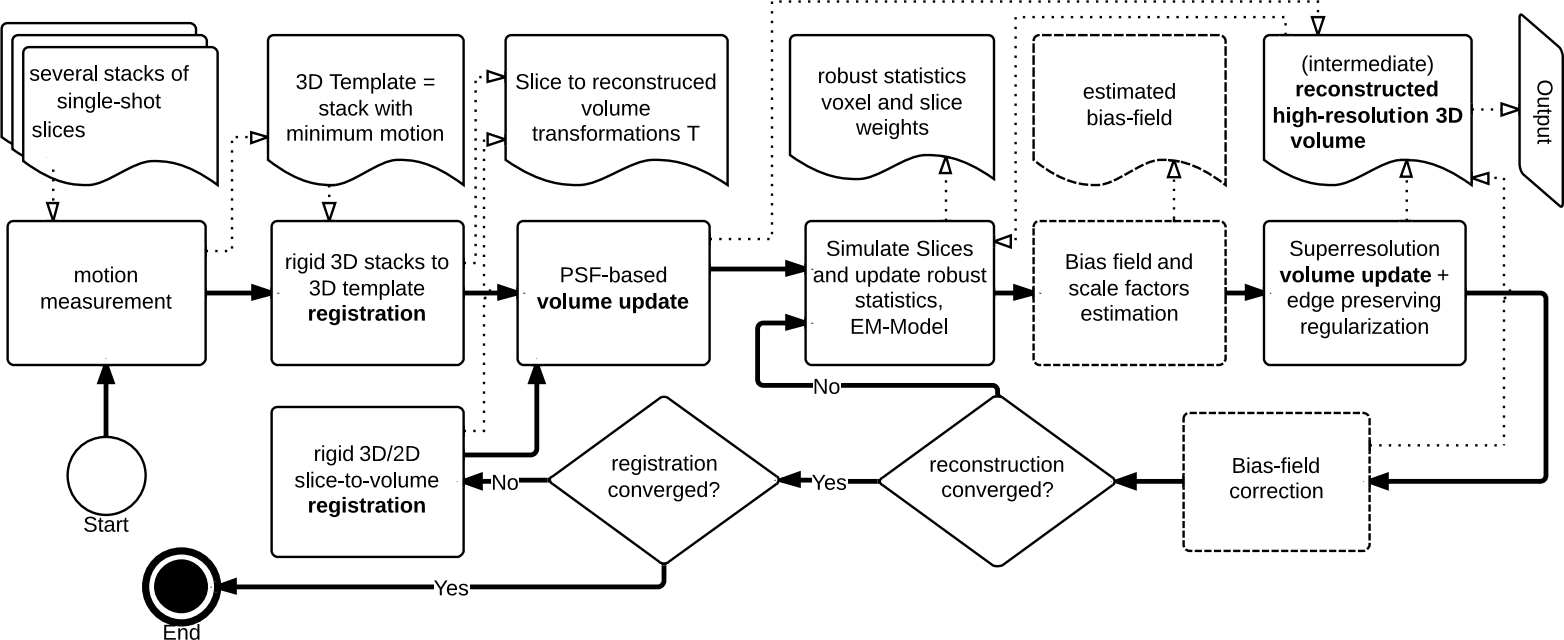
\includegraphics[width=1.0\textwidth]{images/background/svr_overview.png}
    \caption{SVR Overview. From \cite{gpureconstruction}}
    \label{fig:svroverview}
\end{figure}

The first step in the reconstruction is to find the stack with the least movement; this is then used as a target to register the other slices to. Continuous point spread functions (PSFs) are used to model each of the input stacks which allows an initial reconstructed volume to be sampled from the registered slice stacks.

An outlier detection phase is then performed; this involves the inverse transform for every slice stack to the volume being used to simulate what the slice should have looked like, based on the reconstruction. These simulated slices can then be compared to the originals to classify each point into inliers or outliers and EM (Expectation Maximization) is used to give weightings to each voxel.

An update step is then applied to minimize the sum of squared errors between the slice pixels and the simulated slice values; gradient descent is applied to minimize the effect of noise and an edge preserving component is added to aid continuity in the resulting image.

The overall aim of this process is to align each of the slice stacks in a way that minimizes the error due to movement and to build a higher resolution image by combining each of the stacks. This process of combining many lower resolution stacks to create one high resolution image is known as super-resolution.

With super-resolution the images must be taken such that the translation between them is known to sub-pixel accuracy. Having images where the pixels are interleaved in this way allows a higher resolution image to be constructed using interpolation. See figure \ref{fig:superresolution}.

\begin{figure}[H]
    \centering
	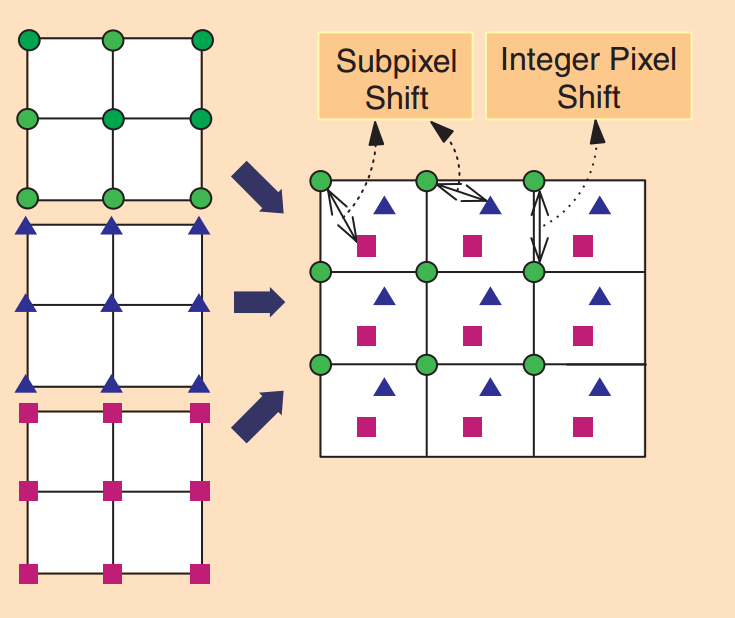
\includegraphics[width=0.8\textwidth]{images/background/super_resolution.png}
    \caption{Low resolution images aligned to sub-pixel accuracy. Adapted from \cite{superresolution2}}
    \label{fig:superresolution}
\end{figure}

\subsection*{Super-Resolution Overview}
The simplest form of super-resolution follows three steps:

\begin{enumerate}
	\item Registration
	\item Interpolation
	\item Post-processing
\end{enumerate}

The registration step is where the transformation between each image is established. Crucially this must be known to sub-pixel accuracy and must not be a whole number of pixels. If, for example, we had two images and one was taken exactly 1 pixels width to the right of the other then we see that both images will contain the same information, in effect we can generate one using the other. However, if the second image is known to be taken half a pixel's width to the right then there is the potential to extract more information.

Once we have registered our images we then interpolate points at a higher resolution, using a combination of the pixel values from each image at each point. There are a number of different interpolation algorithms that we can use; for example nearest neighbour or linear interpolation.

We can then perform post-processing on the final image to reduce the noise or blur. For example to reduce noise a Wiener filter can be used\cite{wienerfilter}.

% ------------------------- %
% ------- SVD / PCA ------- %
% ------------------------- %
\newpage
\section{SVD \& PCA}\label{background:svdpca}
The task of finding the next best scan plane given an uncertainty volume is a task that essentially involves fitting a scan plane to a set of uncertain points. SVD (Singular Value Decomposition) is one technique that has been successfully applied to solving this problem\cite{uncertaintysvd}.

SVD  breaks down a matrix, $A$, into three components: $U$, $D$ and $V$.

\begin{align}
& A = UDV* \nonumber \\
& \text{where} \nonumber \\
& A \text{ - the original matrix. (M x N)} \nonumber \\
& U \text{ - a unitary matrix. (M x M)} \nonumber \\
& D \text{ - a diagonal matrix containing the singular values. (M x N)} \nonumber \\
& V* \text{ - the conjugate transpose of V, a unitary matrix. (N x N)} \nonumber
\end{align}

Note that 'Unitary Matrix' means that $UU* = I$ or alternately $U^{-1} = U^T$. This is true where the matrix contains unit vectors.

Note that the 'Conjugate Transpose' ($*$) of a matrix is just the transpose of the matrix and additionally the complex conjugate of each entry is taken. If the matrix contains no complex values $U* = U^T$.

SVD comes in useful when performing PCA (Principal Component Analysis). PCA is used to take a dataset in $n$ dimensions and map it in such a way that you can describe it in less than $n$, whilst minimizing the information lost.

PCA takes as input a data matrix, X, which is a two dimensional table where each row represents an 'experiment' or 'data point' and each column is a property. Using the covariance of this data, i.e. how much each property varies in relation to every other property, the number of dimensions can be reduced.

To find the principal component we would like find the vector that maximizes the variance in the covariance matrix. This is found by extracting the eigenvalues of the covariance matrix.

\begin{align*}
& X \text{ - data matrix (demeaned)} \\
& XX^{T} \text{ - covariance matrix} \\
& \\
& \text{Since the covariance matrix is symmetric it can be diagonalized.} \\
& \\
& XX^{T} = WDW^{-1} \\
& \\
& W \text{ - eigenvectors of the covariance matrix} \\
& D \text{ - eigenvalues of the covariance matrix} \\
\end{align*}

Applying PCA to $X$ (and using the SVD substitution):

\begin{align*}
X &= UDV^T \\
& \\
XX^T &= (UDV^T)(UDV^T)^T \\
	&= (UDV^T)(VD^TU^T) \\
	&= UDD^TU \\
	&= UD^{2}U \\
	& \text{therefore} \\
UD^{2}U &= WDW
\end{align*}

We see that the eigenvalues are just the square root of the diagonal we get from SVD and the eigenvectors are the same. These eigenvectors form our new dimensions and we can reduce our data to $m < n$ dimensions by picking the m with the largest eigenvalues.

% ------------------------ %
% -------- RANSAC -------- %
% ------------------------ %
\newpage
\section{RANSAC}\label{background:ransac}
RANSAC (Random Sample Consensus) is a technique for estimating model parameters given some sample data. Similarly to SVD it can be used for suggesting the next best scan plane.

Consider the task of trying to fit a line to some data which contains both correct points (inliers) and noisy data (outliers). The problem with simply minimizing the sum of squared errors to all of the points is that the outliers will distort the result such that the inliers are not perfectly described by the data. See figure \ref{fig:ransac}.

\begin{figure}[H]
    \centering
	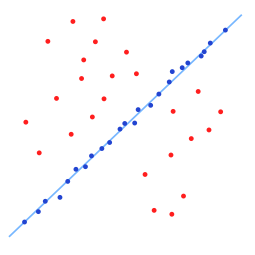
\includegraphics[width=0.4\textwidth]{images/background/ransac.png}
    \caption{Inliers are shown in blue, outliers shown in red. From \cite{ransac:image}}
    \label{fig:ransac}
\end{figure}

RANSAC gets over this problem using random sampling and iteration. It relies on there being more inliers than there are outliers so that statistically inliers will be chosen more frequently. The algorithm is composed of two steps which are repeatedly applied.

As many points are taken randomly from the data set as are needed to fully specify the model (e.g. you need two points to specify a line).

The points are then fit to the model and then all of the data points are compared to this model. If they differ by more than a threshold value they are discarded. If they fit the model they are put into this iterations ‘inlier set’.

A number of iterations are then performed and the winning iteration is the one with the largest inlier set. The final model is then either the model which gave the largest inlier set or alternatively the model can be generated using every point in the inlier set. This algorithm relies on certain parameters being tweaked to perform well:

\begin{itemize}
	\item threshold (how picky to be when discarding points)
	\item iterations (how many times to run the algorithm)
\end{itemize}

% -------------------------- %
% ---- Volume Rendering ---- %
% -------------------------- %
\newpage
\section{Direct Volume Rendering}\label{background:volumerendering}
MRI is a tomographic imaging technique which means that a 3D image is acquired in slices. The resulting scan is created by combining these slices to build a 3D volume. An MRI scan is often displayed in 2D by taking each slice and displaying it, however it is also possible to take all of the slices and view the scan in 3D. One technique for doing this is direct volume rendering.

Direct volume rendering is a technique for visualizing 3D volumetric data which does not generate any intermediate representation. The process uses ray tracing whereby rays are fired through each pixel in the image and properties of light, such as colour and opacity, are modelled to render the data \cite{nvidia:volumerendering}.

One ray is sent into the volume per pixel in the resulting visualization and samples are taken at regular intervals. Each sample point may not exactly hit a voxel in the volume and so the value will be interpolated from the neighbouring points. Linear interpolation can be used but may introduce some visual artefacts in which case more complex interpolation (such as piecewise cubic polynomials) can be used.

Each of these samples, which are just intensity values, need to be mapped to something that we can visualize. A transfer function is used to map intensity values to a colour and transparency. This transfer function can then be changed to highlight different features of our volume, for example we could make all values below a certain threshold completely transparent.

All of the samples along the ray are then combined to calculate the value of the pixel.

\begin{align*}
	C &= \sum\limits_{i=1}^n C_{i}\prod\limits_{j=1}^{i-1}(1 - O_j) \\
	O &= 1 - \prod\limits_{j=1}^n(1 - O_j) \\
	& \text{where} \\
	C_i &= \text{ colour at sample i} \\
	O_j &= \text{ opacity at sample j} \\
	C &= \text{ final colour} \\
	O &= \text{ final opacity}
\end{align*}

Note that if $O$ is greater than 0 then the colour is normalized (divided by $1 - O$).

% ---------------------------- %
% ---- Surface Extraction ---- %
% ---------------------------- %
\newpage
\section{Surface Extraction}\label{background:surfaceextraction}
Surface extraction is another technique that can be used to visualizing volumetric data. Instead of visualizing the data directly, as in direct volume rendering, the volume is processed to build a geometric representation which can then be rendered.

This advantage of using surface extraction is that it is much cheaper to render\cite{surfacevsvolumerendering}. There is an initial penalty where the volume data is processed to extract surfaces but once this has been completed the rendering of geometric primitives is something that can be done rapidly by graphics hardware.

A common surface extraction algorithm is marching cubes. This algorithm works by examining the intensities of neighbouring voxels to tell whether or not the surface passes between them by comparing the values to a threshold value. 

The process is easier to visualize in 2D (marching squares), see Figure~\ref{fig:marching_squares}, but it can be simply extended to 3D.

\begin{figure}[H]
    \centering
	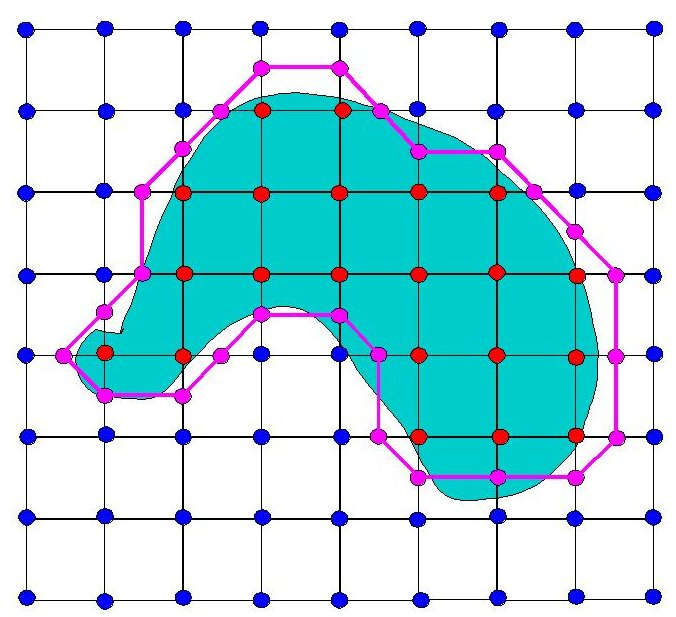
\includegraphics[width=0.8\textwidth]{images/background/marching_squares.jpg}
    \caption{Using marching squares. From \cite{marching_squares:image}}
    \label{fig:marching_squares}
\end{figure}

The marching cubes algorithm generates as a result a mesh of triangles which can be reduced to the desired resolution by applying some mesh decimation techniques.

There are some constraints associated with using surface extraction for volume visualization. Firstly the number of primitives required to represent certain volumes may be prohibitively high. As an extreme imagine trying to extract surfaces from the volumetric representation of a dust cloud; in this case due to the shear quantity of particles it would not be practical to do so and in other situations an accuracy/efficiency trade off must be found. There is also a certain amount of information loss with this technique: importantly individual intensity values are lost.

% ----------------------------------- %
% ---- Uncertainty Visualization ---- %
% ----------------------------------- %
\newpage
\section{Uncertainty Visualization}\label{background:uncertaintyvisualization}
Generally speaking uncertainty visualization tackles the problem of trying to represent the ambiguity or uncertainty in a data set or model. Most data visualization techniques implicitly assume that all of the data being used is perfect and because of this create visualizations that misleadingly represents values with greater precision than the underlying data is known to\cite{uncertaintyoverview}.

One of the reasons that a lot of visualizations neglect this is because it can be quite a difficult task. When creating a visualization there is an inherent restriction on the number of dimensions that you can exploit to represent information.

Consider the general problem of creating a visualization from an n-dimensional dataset in 3D. In this case we need to find a mapping from each dimension in our data to a 'dimension' in our visualization. The dimensions we can control are space (x, y, z), colour (RGB/HSV) and time. The art of data visualization is to find an intuitive mapping to these and to creatively reuse these dimensions to illustrate different features.

The issue when it comes to uncertainty visualization is that most of these dimensions have already been used up with the data itself and so finding intuitive representations for uncertainty is difficult.

To get an idea of what is possible with visualization techniques here are some examples that have been applied successfully in the past.

\begin{figure}[H]
    \centering
	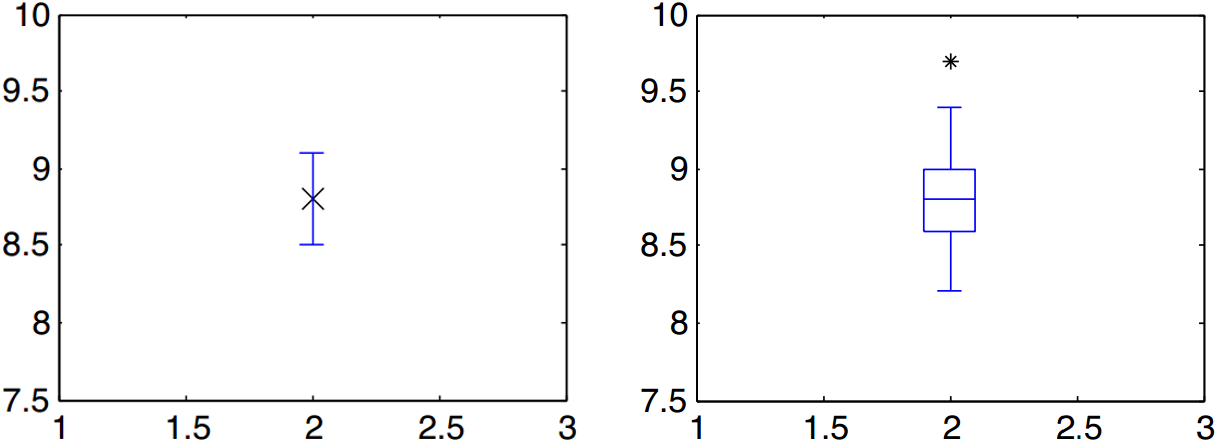
\includegraphics[width=0.8\textwidth]{images/background/error_bars.png}
    \caption{Left: Error Bar, Right: Box and Whisker Plot. From \cite{uncertaintyoverview}}
    \label{fig:error_bars}
\end{figure}

Error bars are possibly the simplest form of uncertainty visualization possible and are commonly found on graphs. They make use of one spatial dimension. An extension of this technique is the box and whisker plot which adds some idea of variance and range. An example of both is shown in Figure~\ref{fig:error_bars}.

\begin{figure}[H]
    \centering
	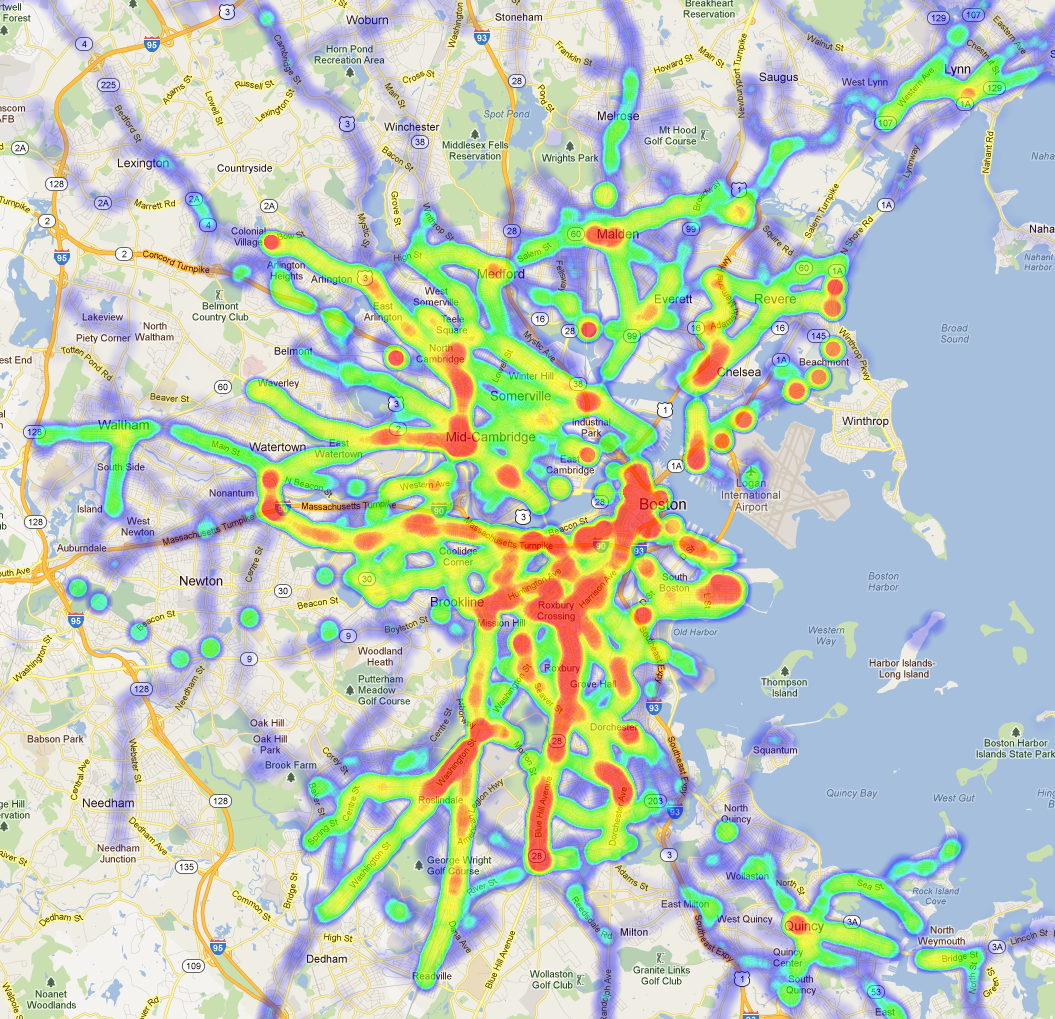
\includegraphics[width=0.4\textwidth]{images/background/heatmap.png}
    \caption{An example heatmap. From \cite{heatmap}}
    \label{fig:heatmap}
\end{figure}

Colour can be very effective at communicating information. A heatmap uses a range of colours to represent intensity data in a certain range. Transparency can also be used though care must be taken to not over complicate the visualization. An example of using both colour and transparency is shown in Figure~\ref{fig:heatmap}.

Time is a useful dimension to exploit but is more suited to some visualizations than others. When combined with a different dimension, such as colour, an animation can be produced that can draw the viewers attention.

In particular a team at the Vienna University of Technology have written a paper on 'attractive flicker' which is designed to draw the viewers attention to a particular point in a cluttered scene\cite{attractiveflicker}. Figure~\ref{fig:flicker} illustrates this idea.

\begin{figure}[H]
    \centering
	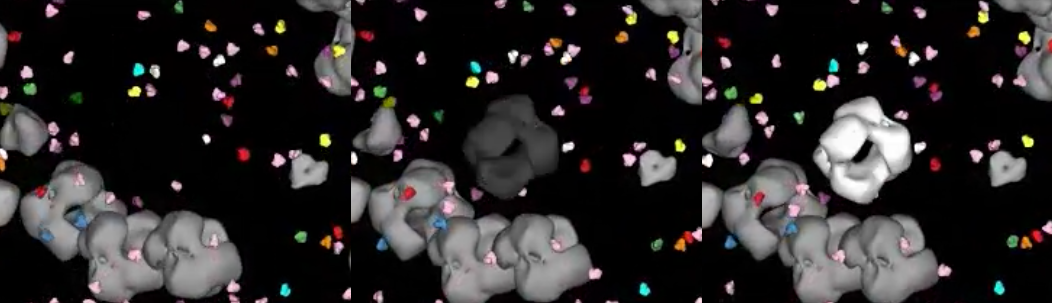
\includegraphics[width=0.8\textwidth]{images/background/flicker.png}
    \caption{Three frames show a molecule being highlighted as it flickers. From \cite{attractiveflicker}}
    \label{fig:flicker}
\end{figure}

When visualizing uncertainty the extreme to draw attention to should be considered. A lot of uncertainty visualizations focus on high uncertainty areas, for example brighter colours on a heatmap or larger error bars, but it may be the case that the viewer is interested in areas of low uncertainty as this is what they can draw conclusions from.

\chapter{Implementation - Tool}
This project has been implemented as an MITK plugin. MITK, the Medical Imaging Interaction Toolkit, is a free open-source software system for the development of interactive medical image processing software. It combines ITK (for image processing) and VTK (for visualization) together and provides a basic application, the MITK Workbench, that can be extended with plugins.

\begin{figure}[H]
  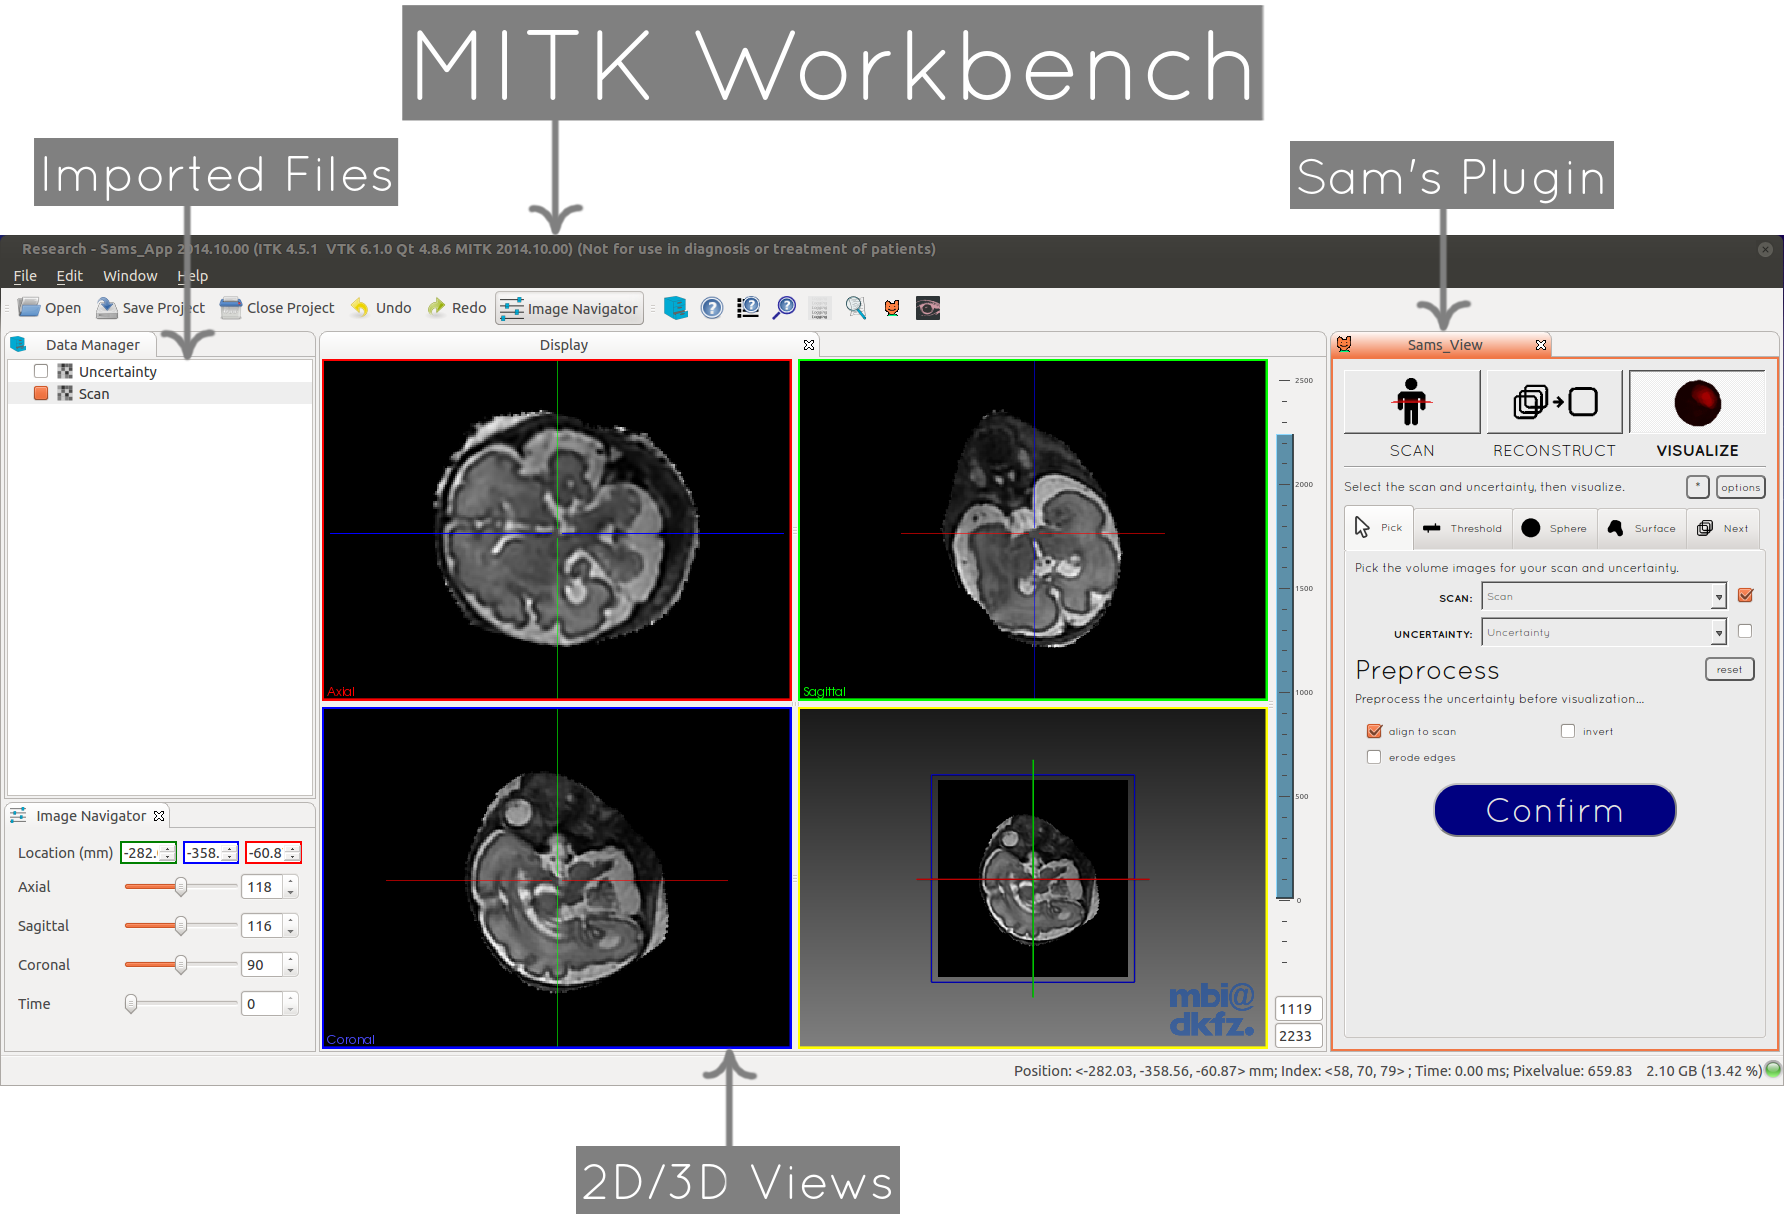
\includegraphics[width=\textwidth]{images/tool/mitk.png}
  \caption{MITK Workbench + Plugin}\label{fig:scansettings}
\end{figure}

The plugin that has been developed is a research prototype designed primarily to visualize the uncertainty in MRI reconstructions. However, it also begins to integrate all parts of the reconstruction pipeline together into one application. Broadly speaking the pipeline can be split into three steps: scan -> reconstruct -> visualize. The plugin developed incorporates components from each stage.

\subsection*{Scan Simulation}
Given a previous reconstruction, that is assumed to be a perfect, ground truth, representation, we can simulate a scan by re-sampling it.

\subsection*{Reconstruct}
Using slice stacks (simulated or otherwise) we can reconstruct a super-resolution image. Optionally landmarks can be provided to guide the registration process.

\subsection*{Visualize}
When the reconstruction has finished we can visualize how well it went.
\begin{itemize}
  \item Thresholding
  \item Uncertainty Sphere
  \item Uncertainty Surface
  \item Next Scan Plane
\end{itemize}

\newpage
\section{Scan Simulation}\label{section:simulatescan}
The idea behind simulating a scan is that we can evaluate the performance of reconstruction algorithms if we can compare the result to a known, 'perfect', reconstruction. This idea was used in the same paper concerned with finding the optimum scan plane\cite{uncertaintysvd}. The focus of this part of the tool is not to evaluate the effectiveness of this approach, that is a project in it's own right, but to make this simulation easier to perform and customize for future research.

\begin{wrapfigure}[23]{r}{0.4\textwidth}
  \vspace{-20pt}
  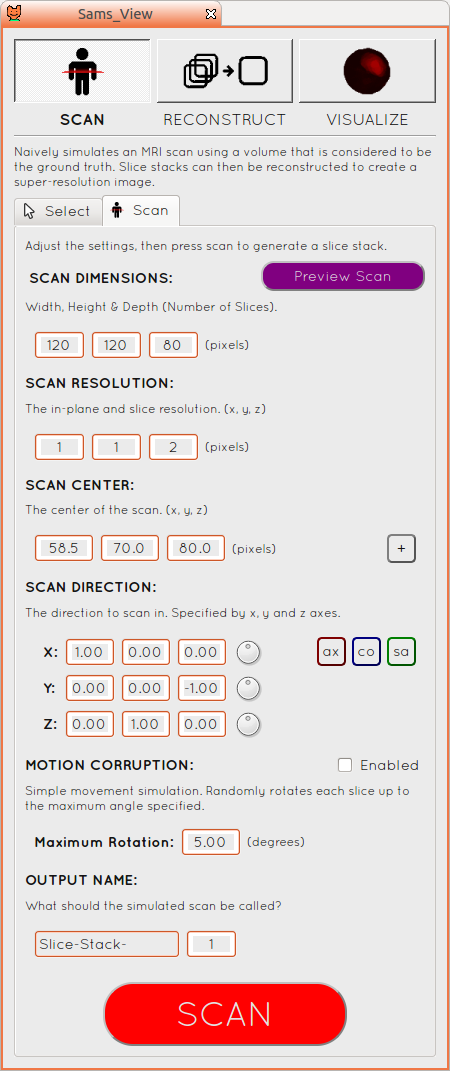
\includegraphics[width=0.4\textwidth]{images/scan_simulation/scan_settings.png}
  \caption{Controls}\label{fig:scansettings}
\end{wrapfigure}

The user has a number of controls (see figure \ref{fig:scansettings}) available to tweak:

\subsection*{Scan Dimensions}
Number of pixels in the scan (x, y, z).

\subsection*{Scan Resolution}
Size of each pixel, relative to the reconstructed scan (x, y, z).

\subsection*{Scan Center}
The center point of the scan (x, y, z). This can be set to the center of the volume or adjusted manually.

\subsection*{Scan Direction}
The direction to scan in. You may expect this to be just one vector (the z-direction) but since the scan is rectangular in shape the x and y-direction also need to be specified. The standard axial, coronal and sagittal directions are available and the direction can be rotated about each axis using the dials.

\subsection*{Motion Corruption}
Some simple motion corruption can be enabled. Currently the implementation is quite simple; the motion only happens in between slices being scanned. Before each slice gets scanned a random rotation (up to a maximum specified) is applied about a random axis to the original image.

Figure \ref{fig:scansimulationexample} shows an example of an axial scan (y-axis) where the preview is overlayed on a volume rendering of the ground truth volume. The preview box shows the boundary of the scan, which is updated to show any changes to the configuration. The effects of the motion corruption are apparent when viewed from the side; successive stacks don't line up.

\begin{figure}[H]
  \centering
  \begin{subfigure}[b]{0.5\textwidth}
    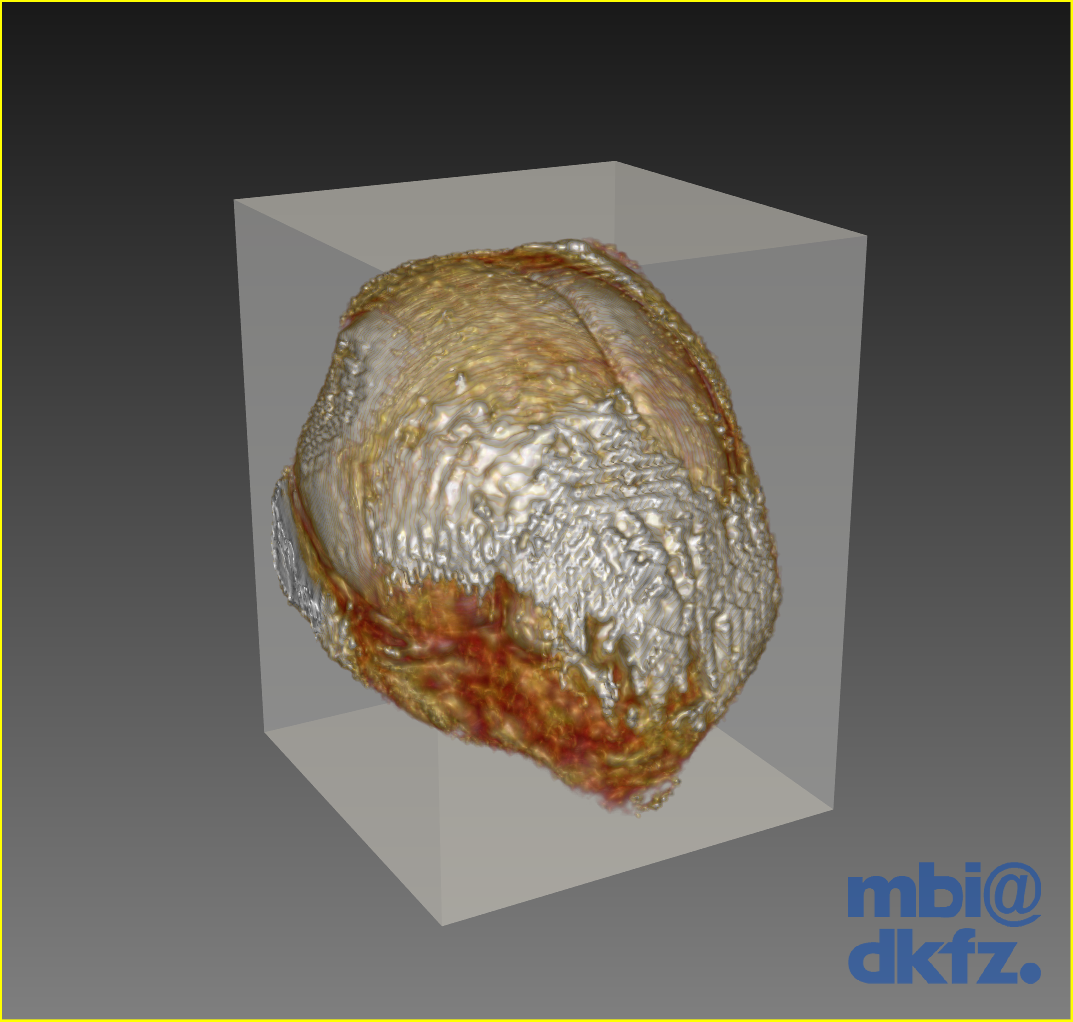
\includegraphics[width=\textwidth]{images/scan_simulation/scan_axial_preview.png}
    \caption{Axial Scan Preview}\label{fig:scansimulationpreview}
  \end{subfigure}%
  ~ %add desired spacing between images, e. g. ~, \quad, \qquad, \hfill etc.
    %(or a blank line to force the subfigure onto a new line)
  \begin{subfigure}[b]{0.5\textwidth}
    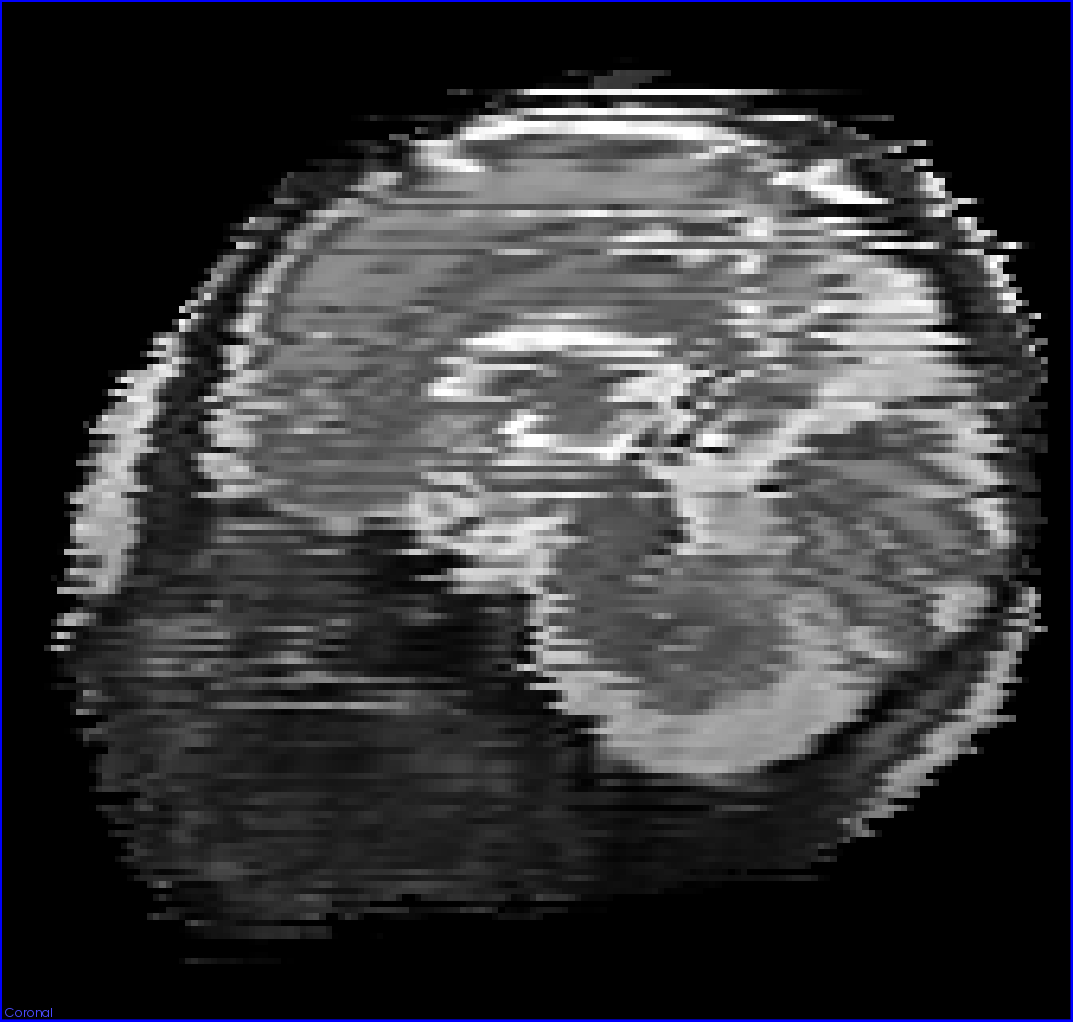
\includegraphics[width=\textwidth]{images/scan_simulation/scan_axial_result.png}
    \caption{Side (Sagittal) View of Simulation}\label{fig:scansimulationresult}
  \end{subfigure}
  \caption{Example Scan Simulation.}\label{fig:scansimulationexample}
\end{figure}

\newpage
\section{Reconstruction}\label{section:reconstruction}
This part of the tool uses the fast GPU reconstruction code developed in \cite{uncertaintysvd}. The Common Toolkit (CTK) includes functionality that allows you to run external binaries from within MITK\cite{ctkcmd}. A wrapper executable has been written, which conforms to the Command Line Module XML Schema, which essentially allows the MITK plugin to make calls to the GPU reconstruction code and automatically import the result.

One of the ways that the quality of the reconstruction can be improved is by manually labelling landmarks in the scans, such as the eyes and extreme points of the skull. This helps the registration step of the reconstruction align each of the initial scans. A prototype to allow each stack to be marked up in this way has been developed with the view of getting the opinion of researchers on whether this is a process they are willing to do, or even if they have the time to do it.

Figure \ref{fig:reconstructionlandmarks} shows the process with some example landmarks. Each landmark can be placed, moved, deleted and you can also jump quickly to a previously marked point.

\begin{figure}[H]
  \centering
  \begin{subfigure}[b]{0.358\textwidth}
    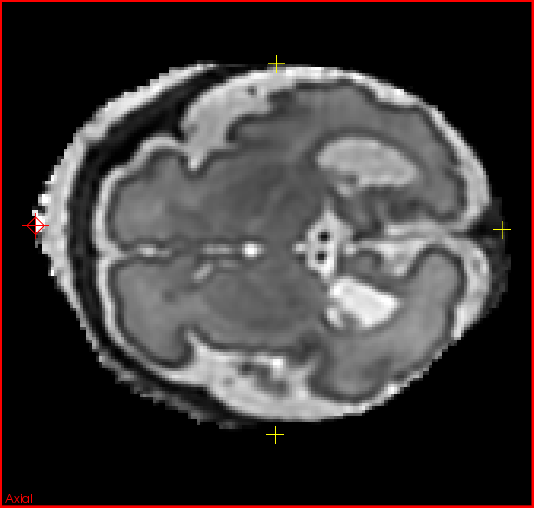
\includegraphics[width=\textwidth]{images/reconstruction/axial.png}
    \caption*{Axial}
    \label{fig:reconstructionaxial}
  \end{subfigure}%
    %add desired spacing between images, e. g. ~, \quad, \qquad, \hfill etc.
    %(or a blank line to force the subfigure onto a new line)
  \begin{subfigure}[b]{0.358\textwidth}
    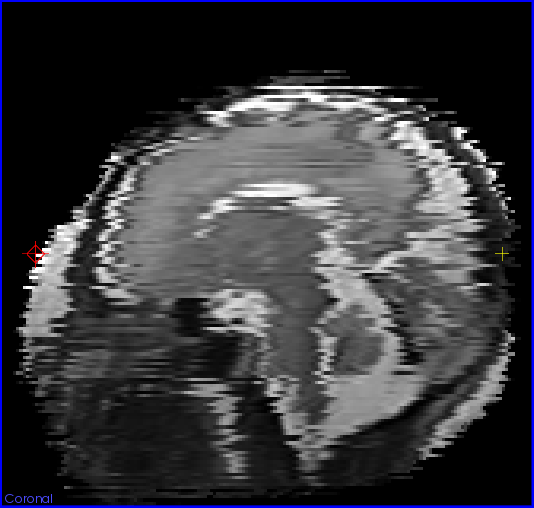
\includegraphics[width=\textwidth]{images/reconstruction/sagittal.png}
    \caption*{Sagittal}
    \label{fig:reconstructionsagittal}
  \end{subfigure}%
    %add desired spacing between images, e. g. ~, \quad, \qquad, \hfill etc.
    %(or a blank line to force the subfigure onto a new line)
  \begin{subfigure}[b]{0.283\textwidth}
    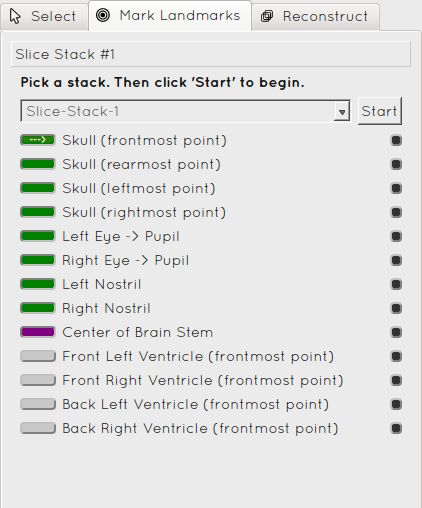
\includegraphics[width=\textwidth]{images/reconstruction/controls.png}
    \caption*{Controls}
    \label{fig:reconstructioncontrols}
  \end{subfigure}
  \caption{Placing Landmarks on Slice Stacks.}\label{fig:reconstructionlandmarks}
\end{figure}

\newpage
\chapter{Implementation - Visualizations}\label{sectiontoolvisualization}
This is where the visualizations live. The demo ones are available.

Show screenshot (annotated).
\begin{figure}[h]
  \centering
  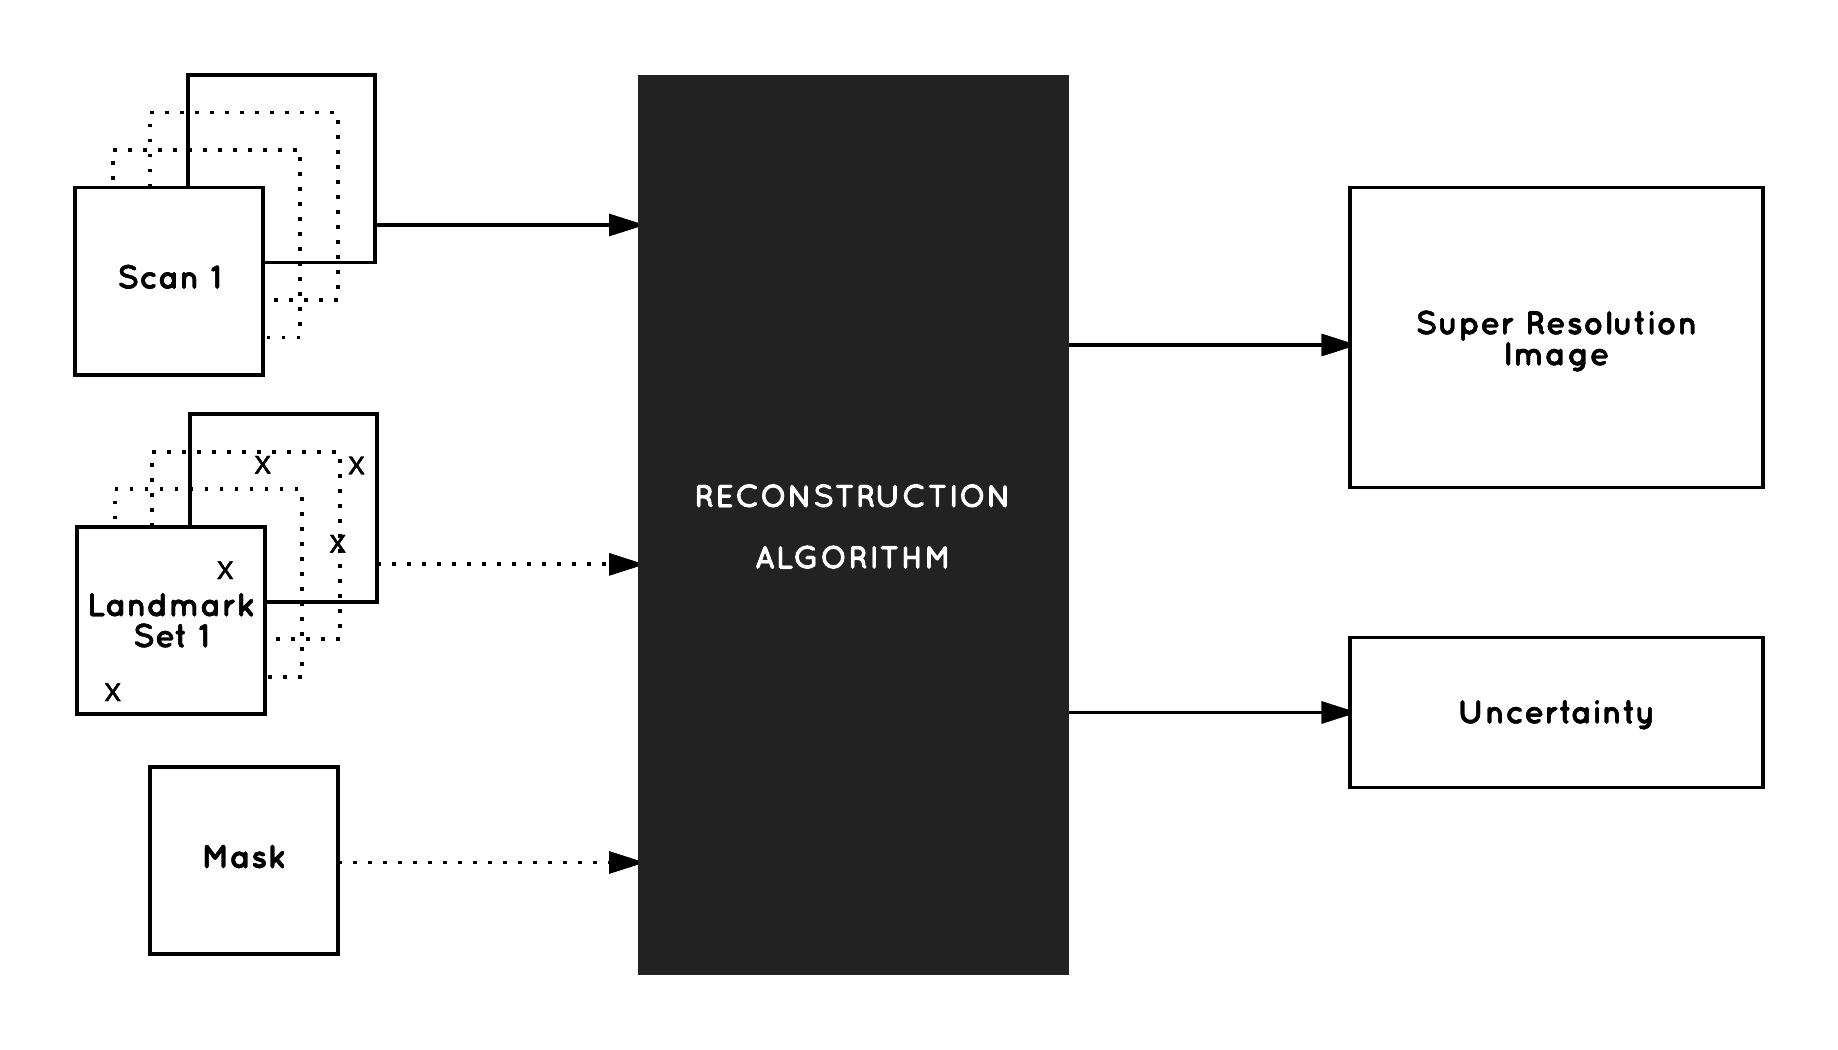
\includegraphics[width=0.8\textwidth]{images/reconstruction_overview.png}
  \caption{Reconstruction Overview}
  \label{fig:erosionbefore}
\end{figure}

The super-resolution reconstruction process takes in a set of slice stacks (scans), an optional mask and outputs the reconstructed MRI volume and the uncertainty. The mask is used to ignore areas that are not of interest; for example when doing a fetal scan a mask can be created to ignore surrounding areas like the womb and amniotic fluid.

\section{Preprocessing}\label{section:preprocessing}
The uncertainty tells us for each pixel in the reconstructed volume how much confidence we have in that value. However, before we can visualize it some preprocessing must be applied. 

\subsection*{Normalization}
The uncertainty is linearly scaled so each value is between 0 and 1.

\begin{verbatim}
  0 - no information (high uncertainty - worst)
  1 - maximum information (low uncertainty - best)
\end{verbatim}

\subsection*{Erosion}
The optional erosion step removes the uncertainty values at the edge of the reconstruction. The edges often have a much higher uncertainty either because there are fewer slices to use or the mask cuts off the data required. Removing this edge helps the visualization to focus on the core of the volume.

The edges are removed in five steps:

\begin{enumerate}
  \item An erosion filter is applied to the image. This removes the edges but has the unwanted effect of also eroding uncertainty in the center of the volume.
  \item The absolute difference is taken between the original and the eroded image.
  \item The difference is then thresholded to create a mask of the areas that changed the most. The idea here is that the edges change significantly more than the small pockets of uncertainty inside.
  \item A growing filter is applied to the mask, to ensure the entire edge is covered.
  \item Finally all the points in the mask are set to 0 to remove the edge.
\end{enumerate}

Figure \ref{fig:erosionoverview} shows how the soft fade out of uncertainty due to the mask is removed to create a hard edge.

\begin{figure}[h]
  \centering
  \begin{subfigure}[b]{0.3\textwidth}
    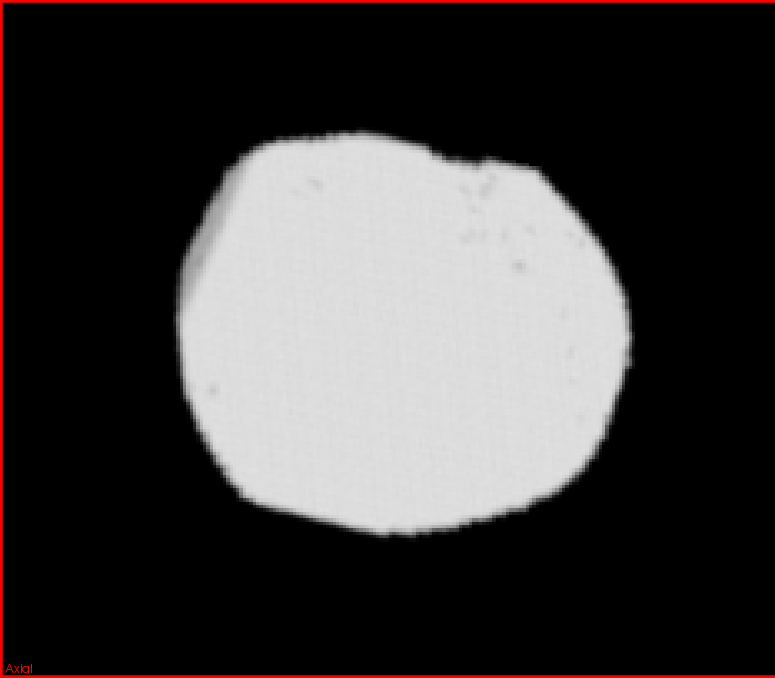
\includegraphics[width=\textwidth]{images/erosion/erosion_0.png}
    \caption{Original}
    \label{fig:erosion0}
  \end{subfigure}%
  ~ %add desired spacing between images, e. g. ~, \quad, \qquad, \hfill etc.
    %(or a blank line to force the subfigure onto a new line)
  \begin{subfigure}[b]{0.3\textwidth}
    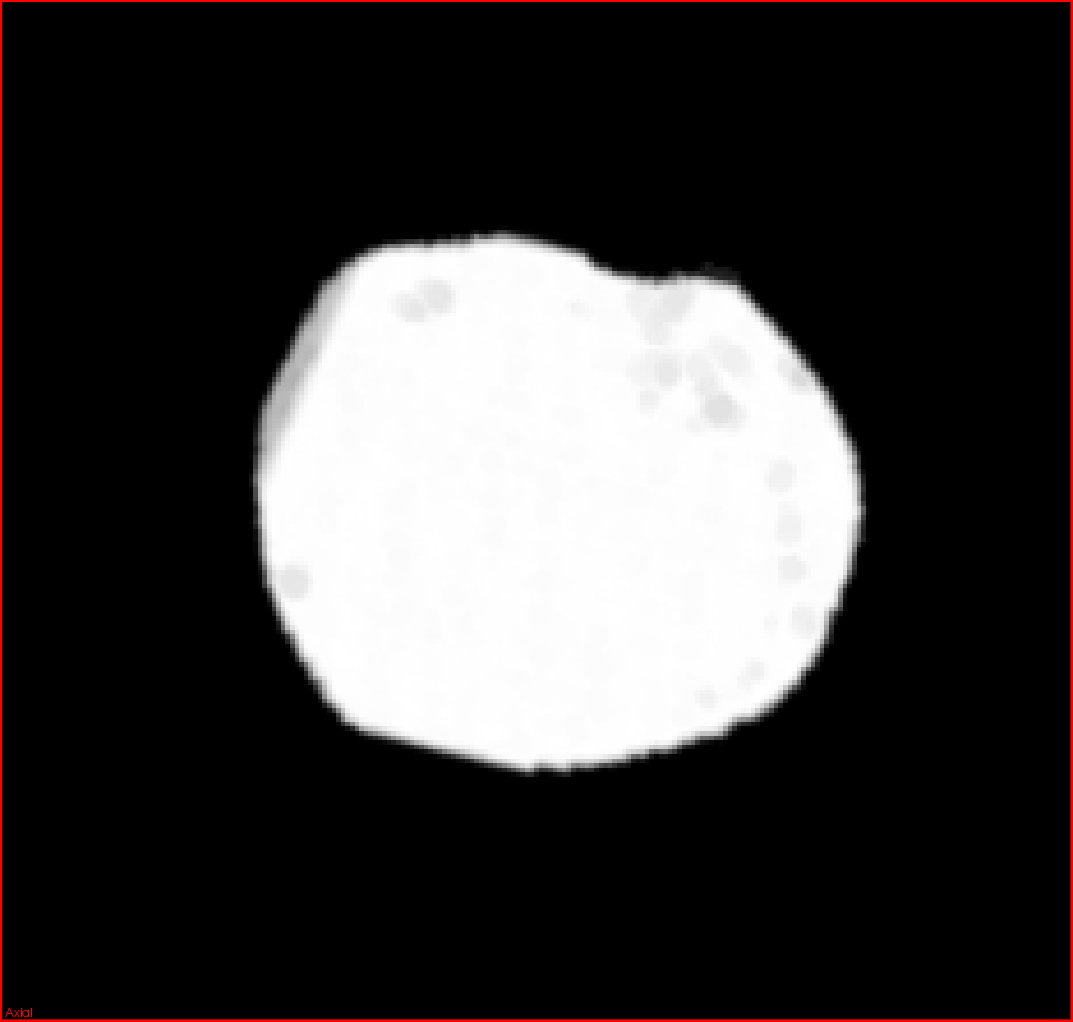
\includegraphics[width=\textwidth]{images/erosion/erosion_1.png}
    \caption{Step 1}
    \label{fig:erosion1}
  \end{subfigure}  
  ~ %add desired spacing between images, e. g. ~, \quad, \qquad, \hfill etc.
    %(or a blank line to force the subfigure onto a new line)
  \begin{subfigure}[b]{0.3\textwidth}
    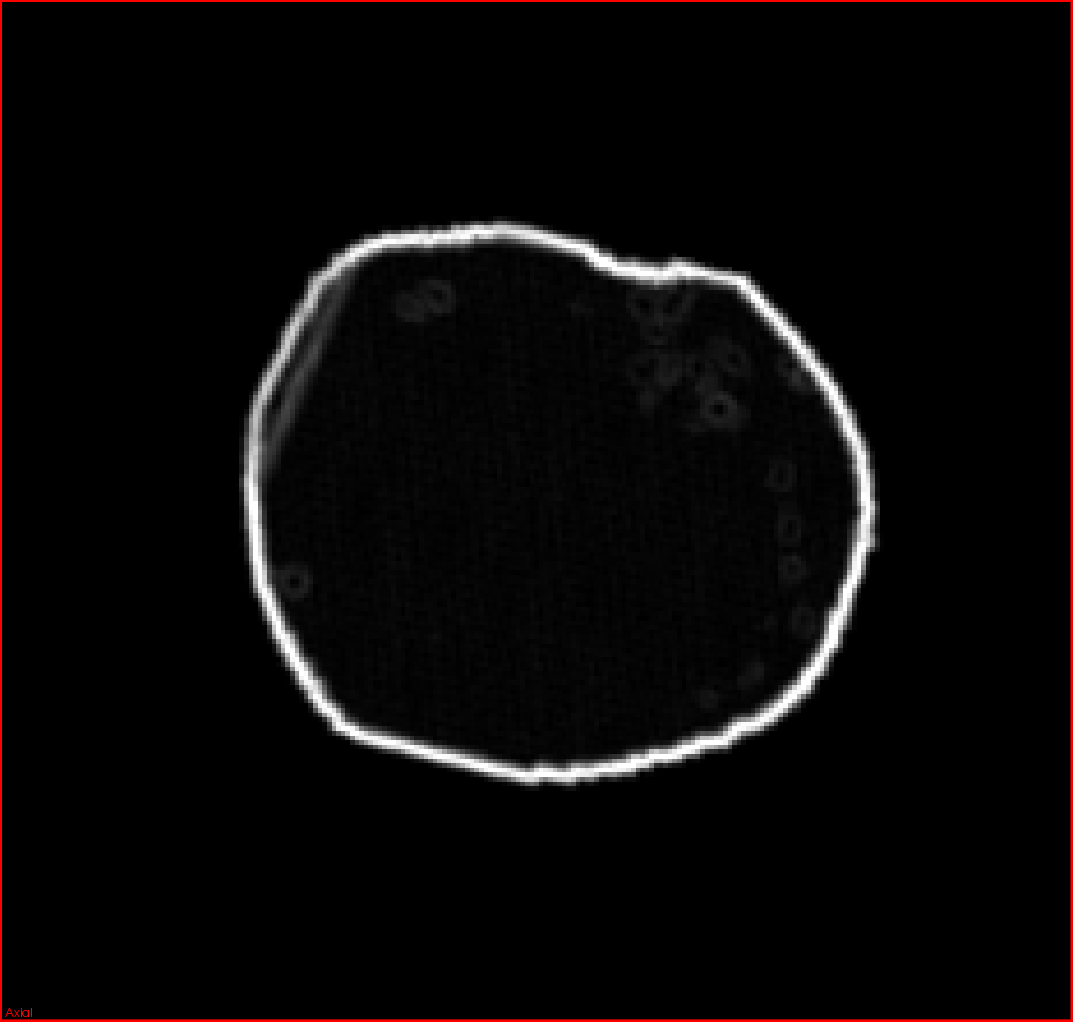
\includegraphics[width=\textwidth]{images/erosion/erosion_2.png}
    \caption{Step 2}
    \label{fig:erosion2}
  \end{subfigure}
  ~ %add desired spacing between images, e. g. ~, \quad, \qquad, \hfill etc.
    %(or a blank line to force the subfigure onto a new line)
  \begin{subfigure}[b]{0.3\textwidth}
    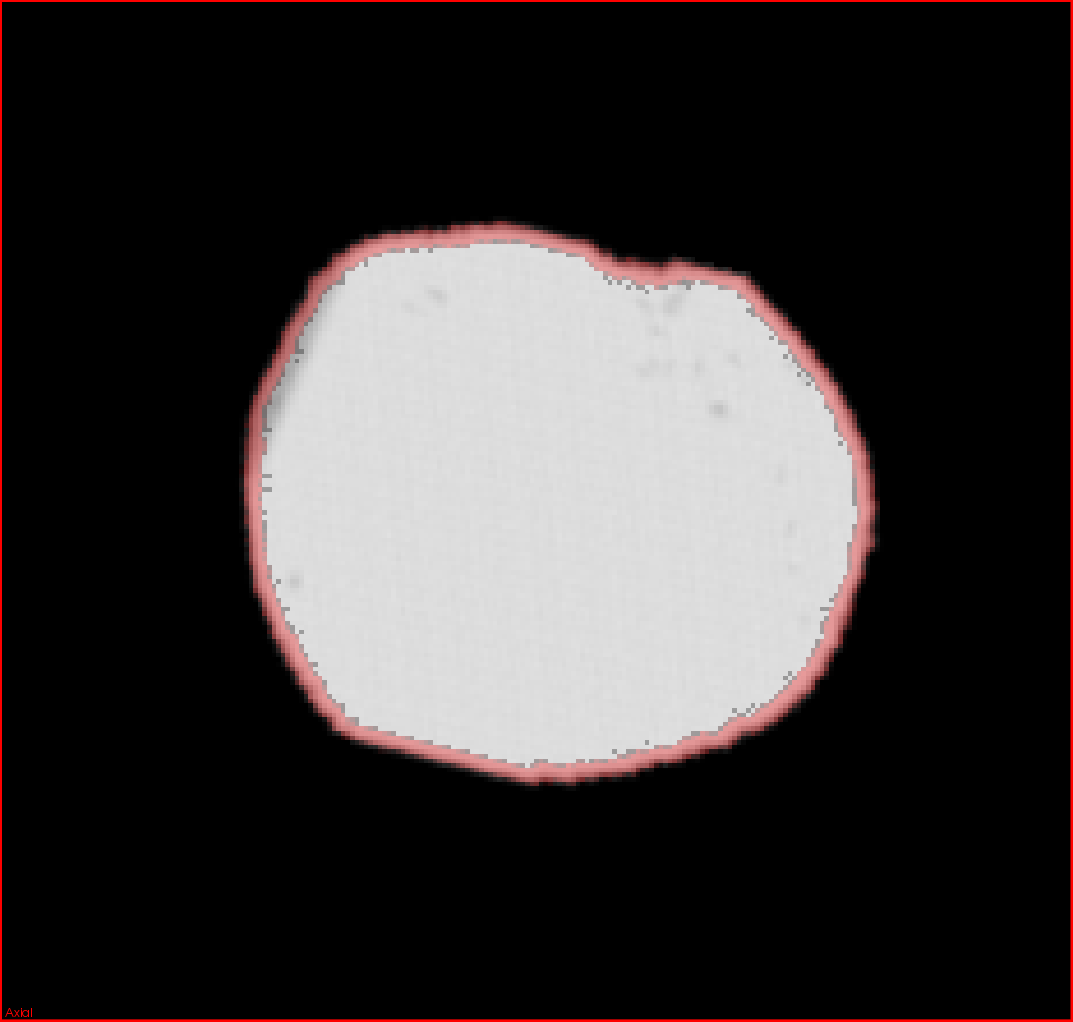
\includegraphics[width=\textwidth]{images/erosion/erosion_3.png}
    \caption{Step 3}
    \label{fig:erosion3}
  \end{subfigure}%
  ~ %add desired spacing between images, e. g. ~, \quad, \qquad, \hfill etc.
    %(or a blank line to force the subfigure onto a new line)
  \begin{subfigure}[b]{0.3\textwidth}
    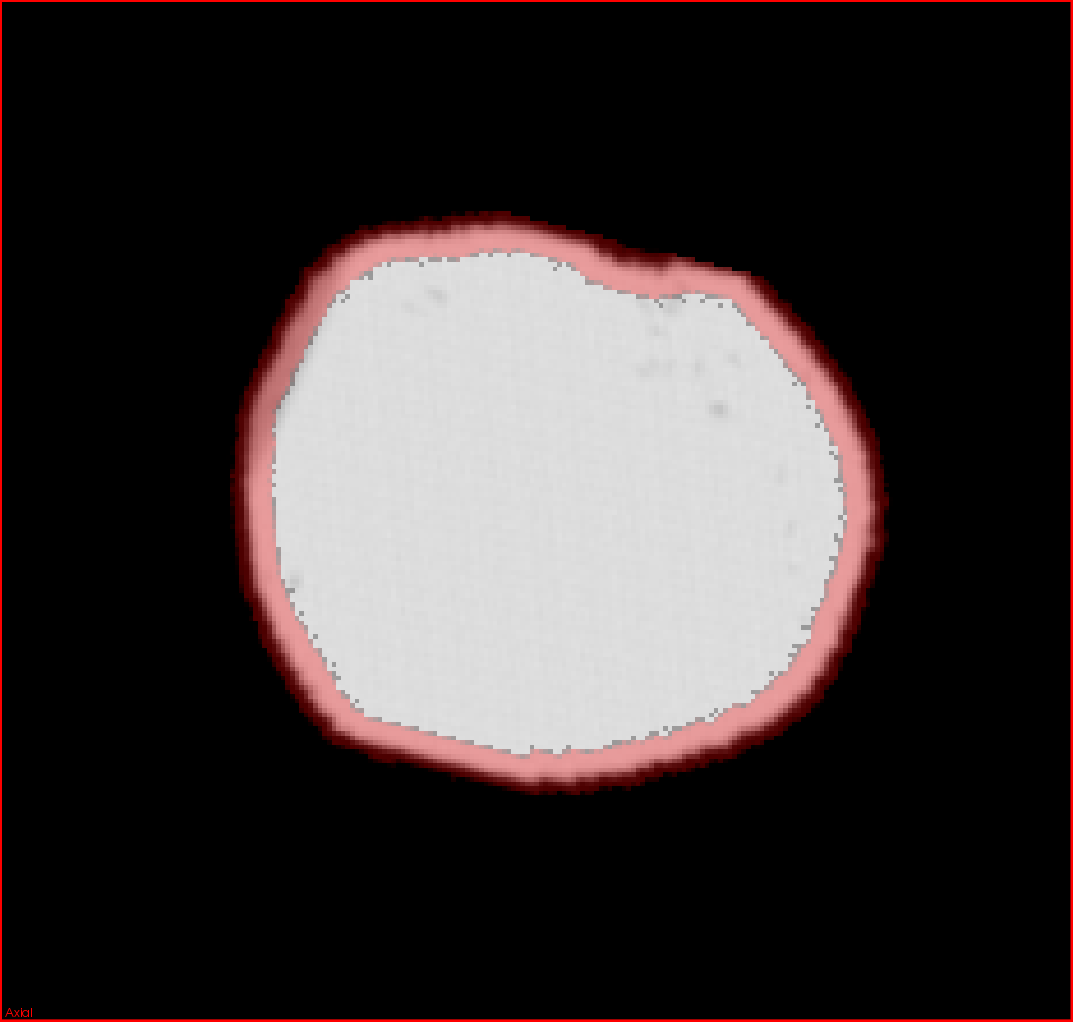
\includegraphics[width=\textwidth]{images/erosion/erosion_4.png}
    \caption{Step 4}
    \label{fig:erosion4}
  \end{subfigure}  
  ~ %add desired spacing between images, e. g. ~, \quad, \qquad, \hfill etc.
    %(or a blank line to force the subfigure onto a new line)
  \begin{subfigure}[b]{0.3\textwidth}
    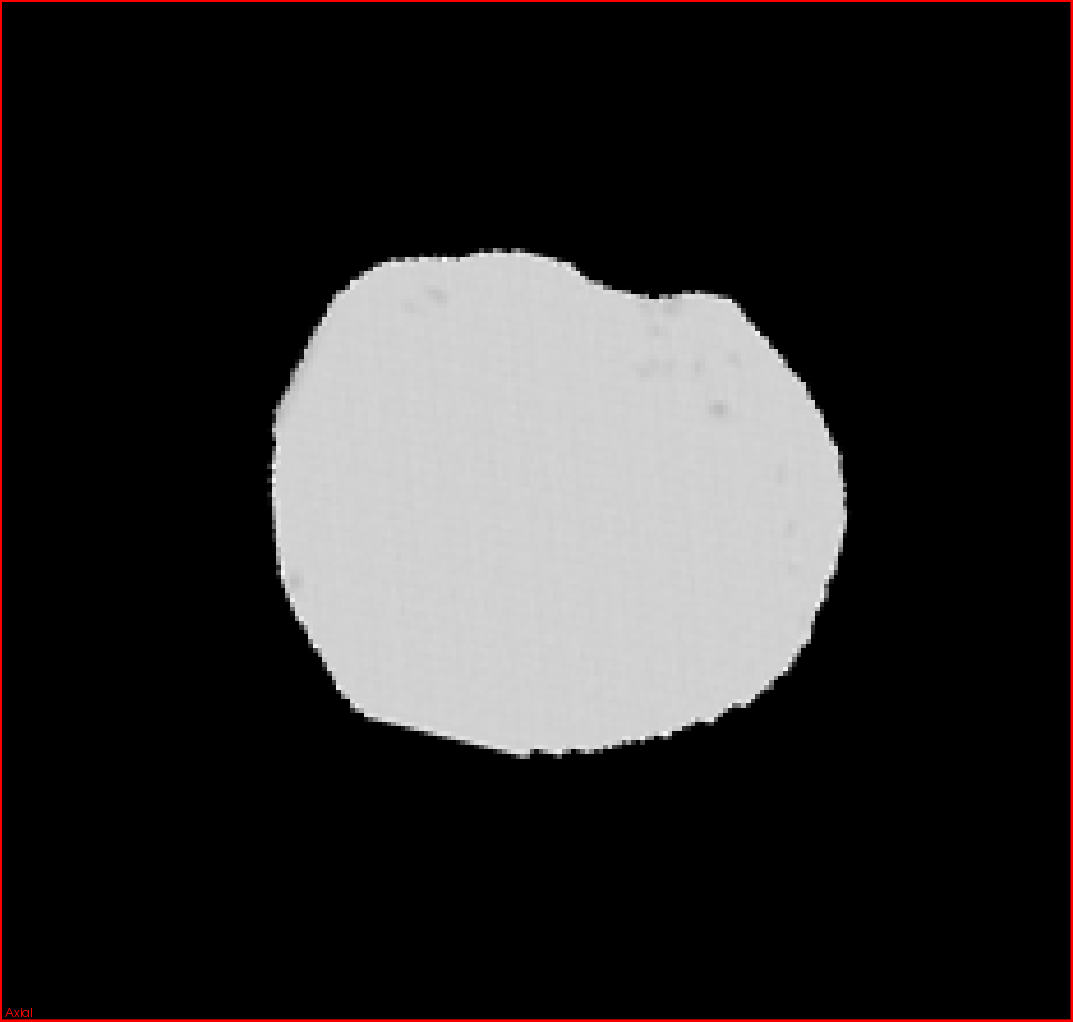
\includegraphics[width=\textwidth]{images/erosion/erosion_5.png}
    \caption{Step 5}
    \label{fig:erosion5}
  \end{subfigure}  
  \caption{Steps involved in removing the edge.}\label{fig:erosionoverview}
\end{figure}

\newpage
\section{Test Uncertainties}\label{section:testuncertainties}

To test the different visualizations during development a number of artificial uncertainty volumes were used, as well as uncertainty from a fetal brain reconstruction.

For each visualization that has been developed the results with these test uncertainties will be examined and compared.

\subsection*{Sphere of Uncertainty}
An uncertainty volume where the uncertainty is proportional to the distance from the center. The uncertainty at the center is 0 (very uncertain) which then goes to 1 (very certain) at the edges.

\subsection*{Sphere in Corner}
Similar to the sphere, but instead of being placed in the middle it is placed in one corner of the volume.

\subsection*{Cube of Uncertainty}
An uncertainty volume that is 1 (very good) everywhere except for fixed size cube of uncertainty 0 (very bad) in the center.

\subsection*{Random Uncertainty}
The uncertainty at every point is a random uniformly distributed value.

\subsection*{Reconstruction Uncertainty}
Uncertainty generated from an example super-resolution reconstruction of a fetal brain.\\

\begin{figure}[h]
  \centering
  \begin{subfigure}[b]{0.18\textwidth}
    \fcolorbox{gray}{white}{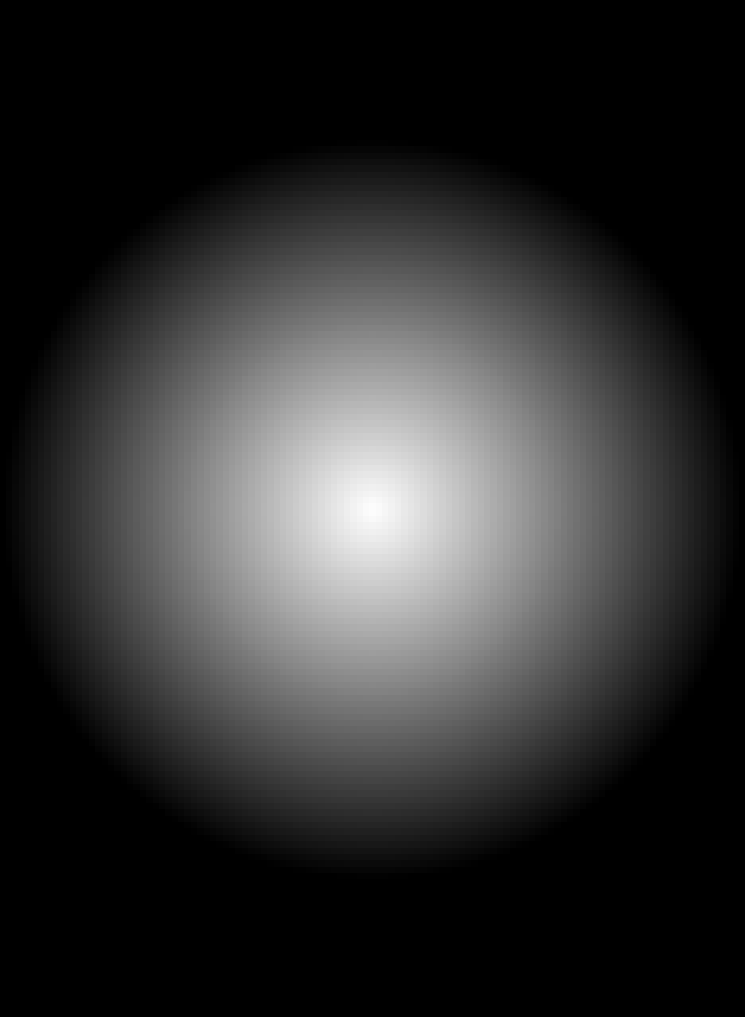
\includegraphics[width=\textwidth]{images/test/test_sphere.png}}
    \caption{Sphere}
    \label{fig:erosion0}
  \end{subfigure}%
  ~~%add desired spacing between images, e. g. ~, \quad, \qquad, \hfill etc.
    %(or a blank line to force the subfigure onto a new line)
  \begin{subfigure}[b]{0.18\textwidth}
    \fcolorbox{gray}{white}{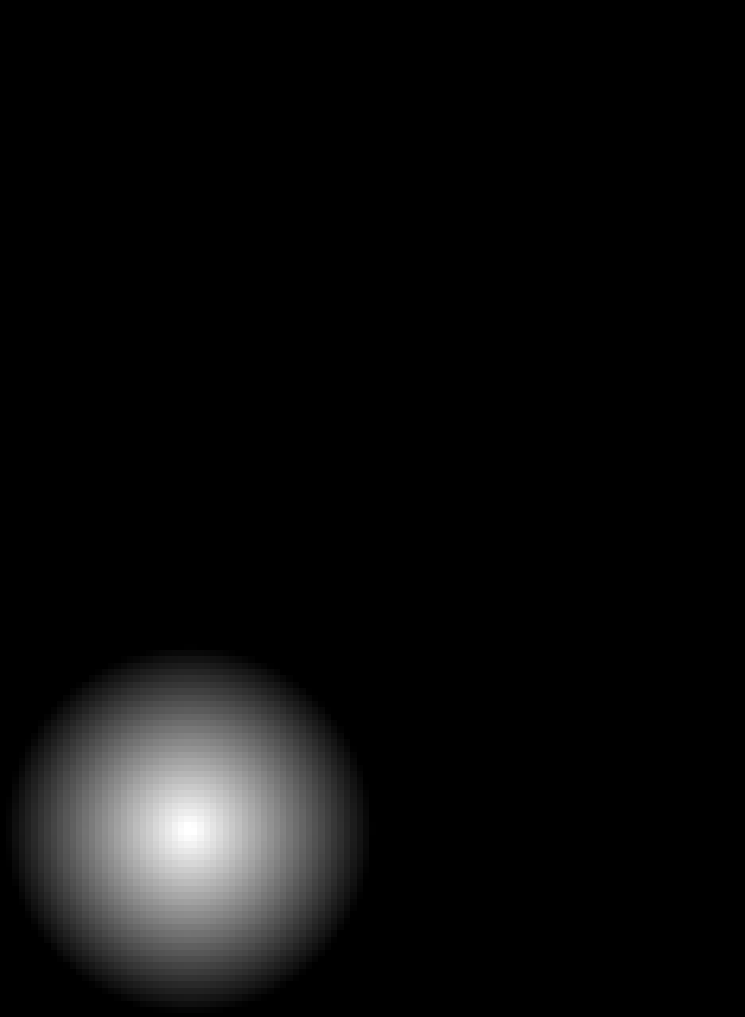
\includegraphics[width=\textwidth]{images/test/test_quadsphere.png}}
    \caption{Corner}
    \label{fig:erosion1}
  \end{subfigure}%
  ~~%add desired spacing between images, e. g. ~, \quad, \qquad, \hfill etc.
    %(or a blank line to force the subfigure onto a new line)
  \begin{subfigure}[b]{0.18\textwidth}
    \fcolorbox{gray}{white}{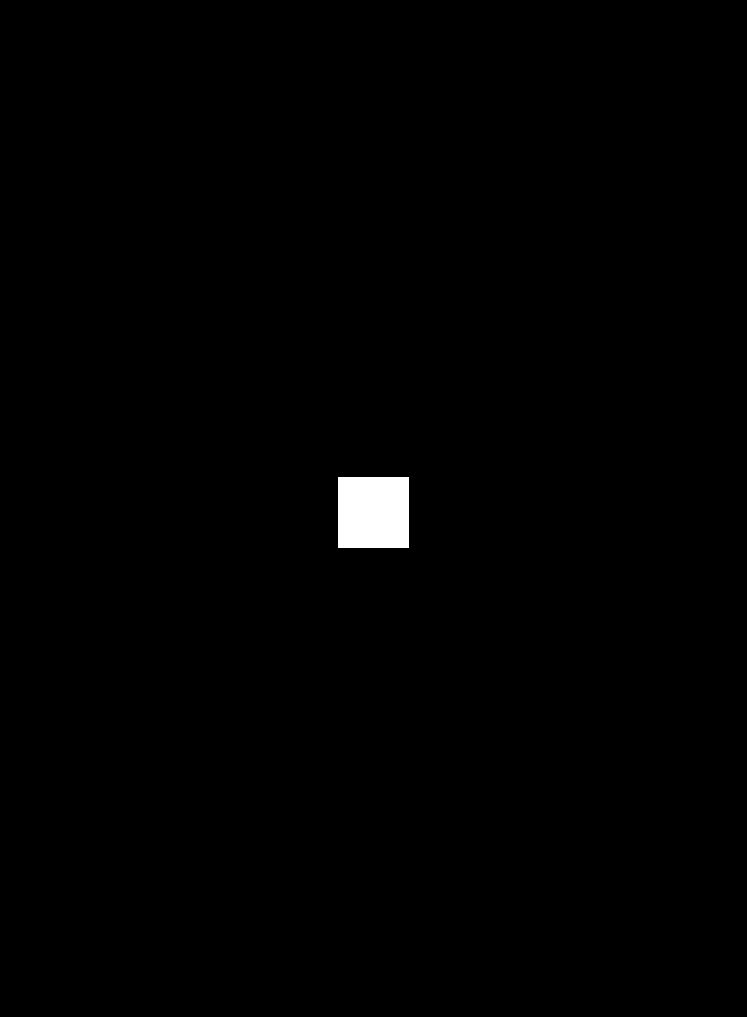
\includegraphics[width=\textwidth]{images/test/test_cube.png}}
    \caption{Cube}
    \label{fig:erosion2}
  \end{subfigure}%
  ~~%add desired spacing between images, e. g. ~, \quad, \qquad, \hfill etc.
    %(or a blank line to force the subfigure onto a new line)
  \begin{subfigure}[b]{0.18\textwidth}
    \fcolorbox{gray}{white}{
\includegraphics[width=\textwidth]{images/test/test_random.png}}
    \caption{Random}
    \label{fig:erosion3}
  \end{subfigure}%
  ~~%add desired spacing between images, e. g. ~, \quad, \qquad, \hfill etc.
    %(or a blank line to force the subfigure onto a new line)
  \begin{subfigure}[b]{0.18\textwidth}
    \fcolorbox{gray}{white}{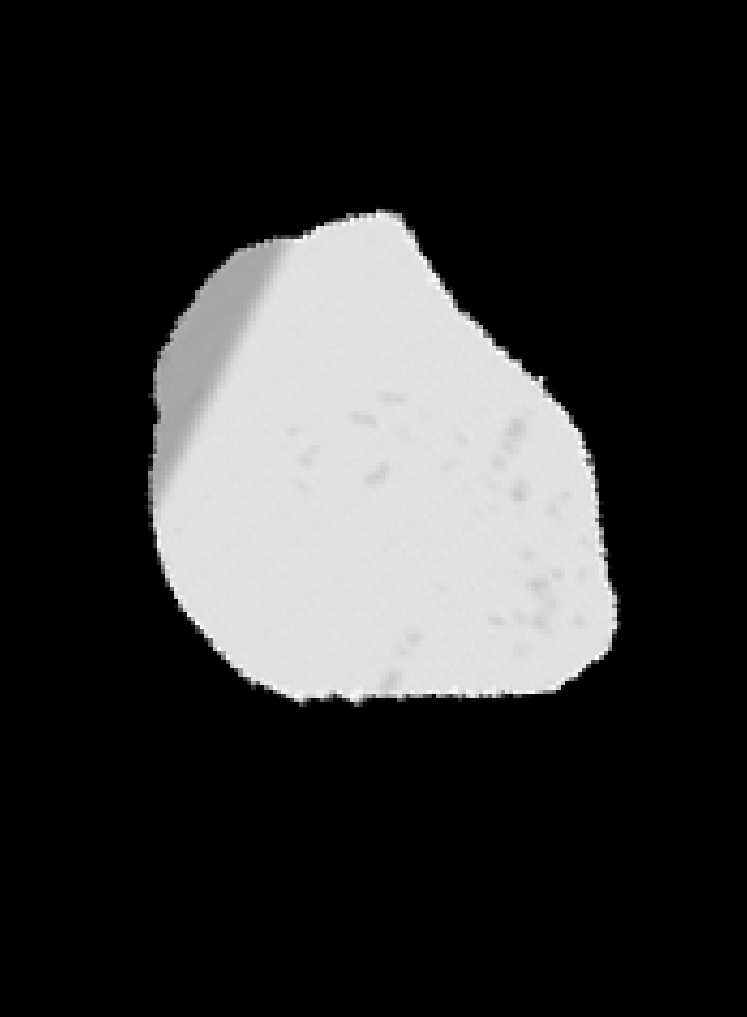
\includegraphics[width=\textwidth]{images/test/test_scan.png}}
    \caption{Fetal Brain}
    \label{fig:erosion3}
  \end{subfigure}
  \caption{Steps involved in removing the edge.}\label{fig:erosionoverview}
\end{figure}

% Idea -> Implementation -> Results
\newpage
\section{Thresholding}\label{section:thresholding}

The idea behind thresholding is to isolate areas in the reconstructed image within a particular range of uncertainty. This allows the viewer to highlight regions in a specified range (e.g. 0.2 to 0.5) and also lets them isolate the worst values in the volume (e.g. the worst 1$\%$).

\subsection*{Implementation}
The implementation uses a filter provided by ITK to go create a binary mask which is set to 1 where the uncertainty is in the range and 0 where it is not. This mask is then overlayed on the reconstructed scan in 2D and made transparent so both the uncertain area and underlying scan can be seen simultaneously. See figure \ref{fig:thresholding2d}.

\begin{figure}[H]
  \centering
  \begin{subfigure}[b]{0.3\textwidth}
    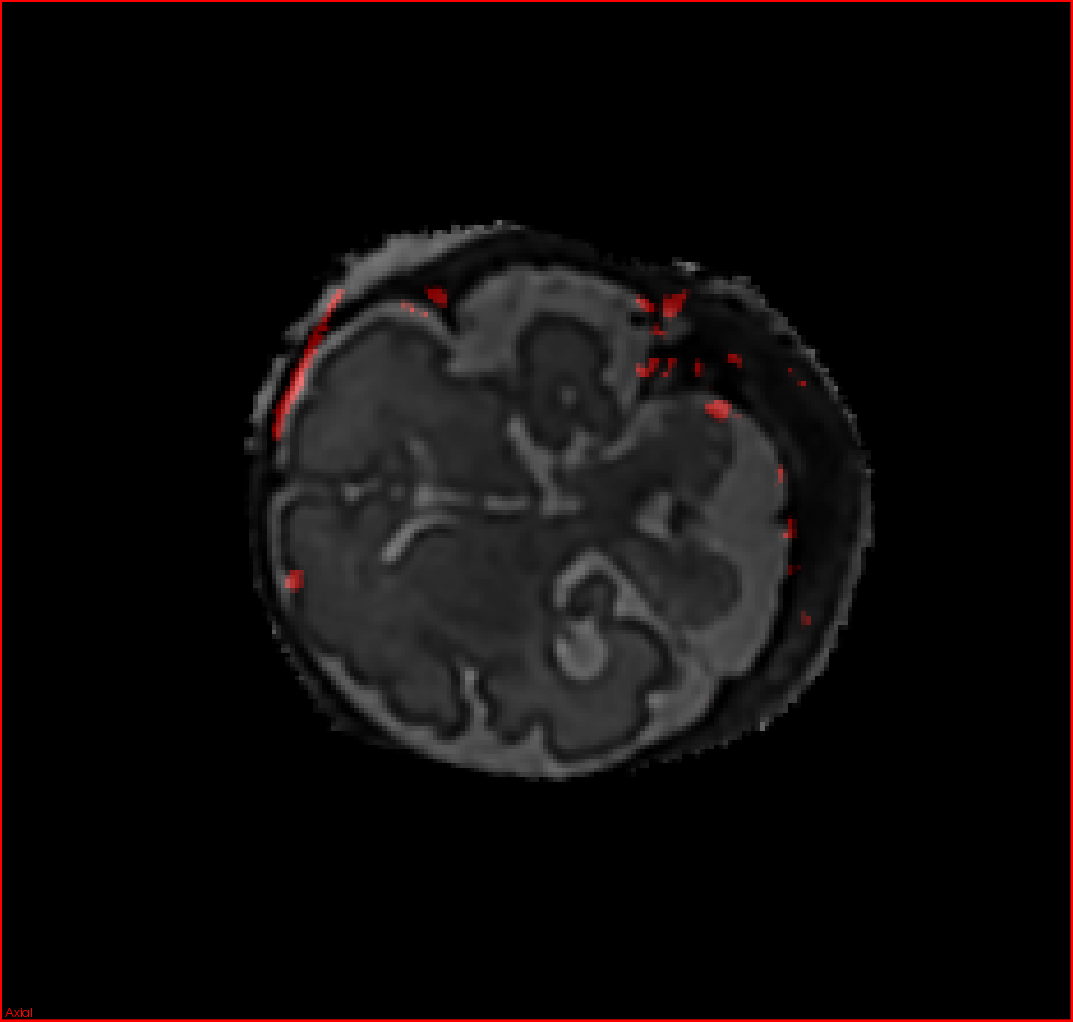
\includegraphics[width=\textwidth]{images/thresholding/thresholding_2d_axial.png}
    \caption{Axial}
    \label{fig:thresholding2daxial}
  \end{subfigure}%
  ~ %add desired spacing between images, e. g. ~, \quad, \qquad, \hfill etc.
    %(or a blank line to force the subfigure onto a new line)
  \begin{subfigure}[b]{0.3\textwidth}
    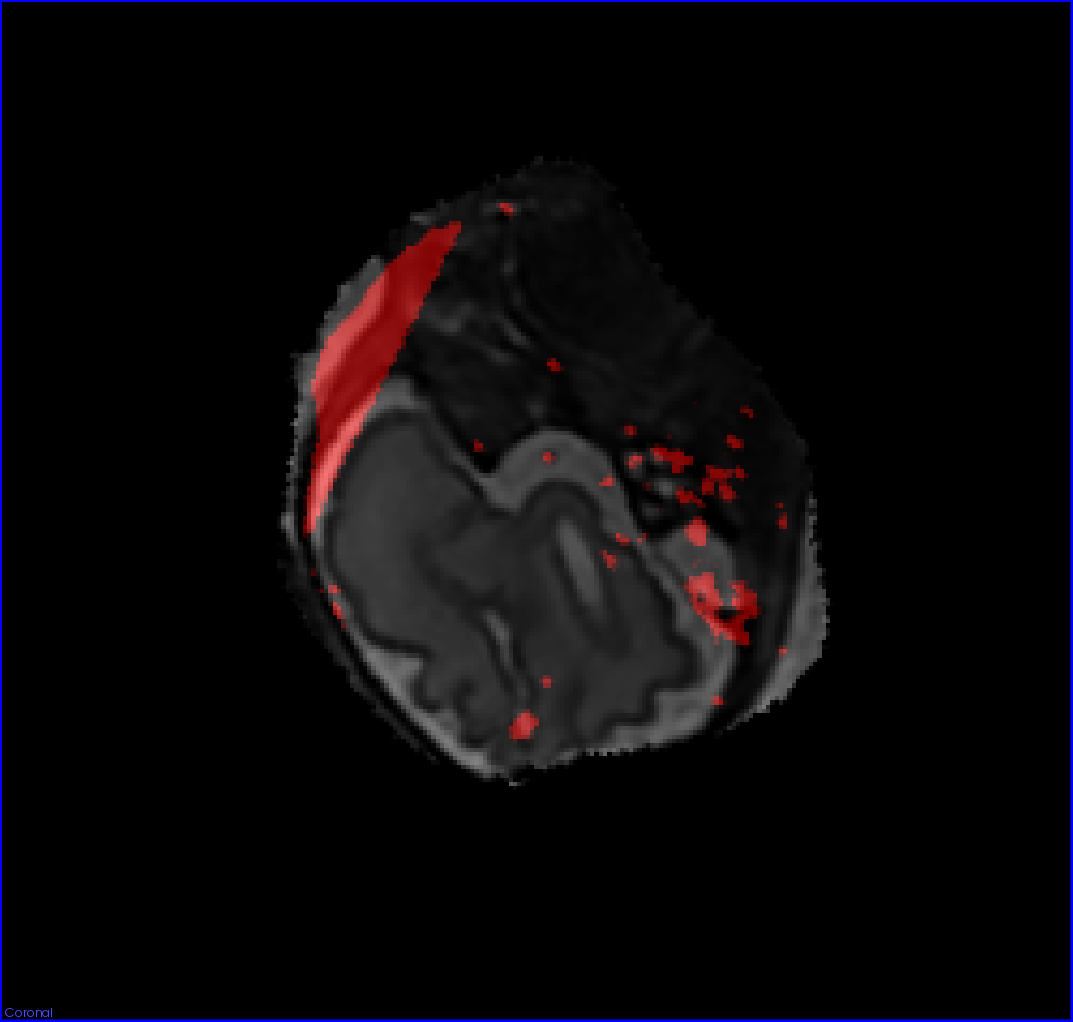
\includegraphics[width=\textwidth]{images/thresholding/thresholding_2d_coronal.png}
    \caption{Coronal}
    \label{fig:thresholding2dcoronal}
  \end{subfigure}%
  ~ %add desired spacing between images, e. g. ~, \quad, \qquad, \hfill etc.
    %(or a blank line to force the subfigure onto a new line)
  \begin{subfigure}[b]{0.3\textwidth}
    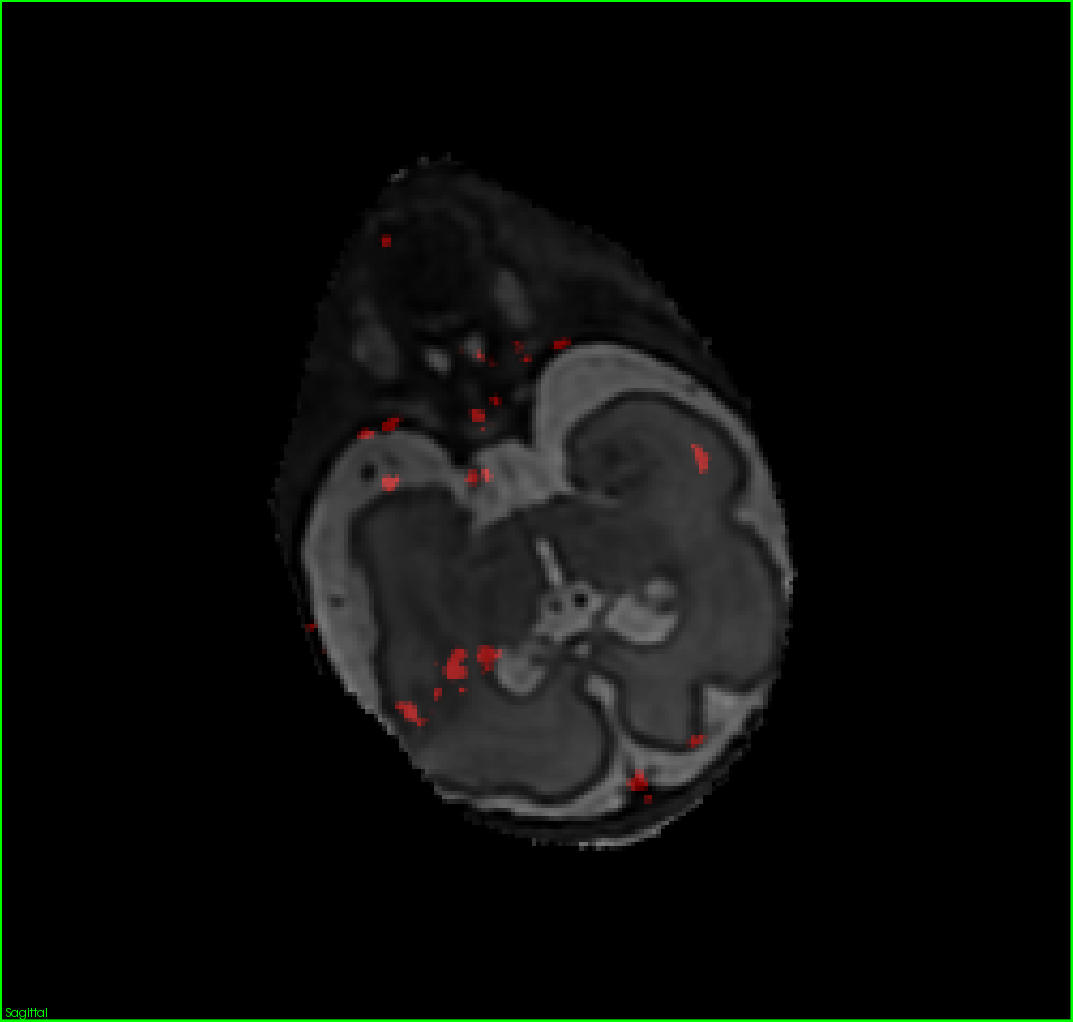
\includegraphics[width=\textwidth]{images/thresholding/thresholding_2d_sagittal.png}
    \caption{Sagittal}
    \label{fig:thresholding2dsagittal}  
  \end{subfigure}
  \caption{Thresholding in 2D}\label{fig:thresholding2d}
\end{figure}

To view the uncertainty in 3D, two variations have been implemented, both using volume rendering (see section \ref{background:volumerendering}). Variation 1 applies volume rendering directly to the uncertainty and variation 2 applies volume rendering to the binary mask.

The transfer functions used in each variation can be seen in figure \ref{fig:thresholdingoverview}. The first works by making values within the thresholded range opaque and those outside it transparent. The second works in a similar way; 0 in the mask is out of the range and 1 in the mask is in the range. In the second transfer function there is a slow fade out, rather than a sharp change, to give individual points of uncertainty some presence.

\begin{figure}[H]
  \centering
  \begin{subfigure}[b]{0.5\textwidth}
    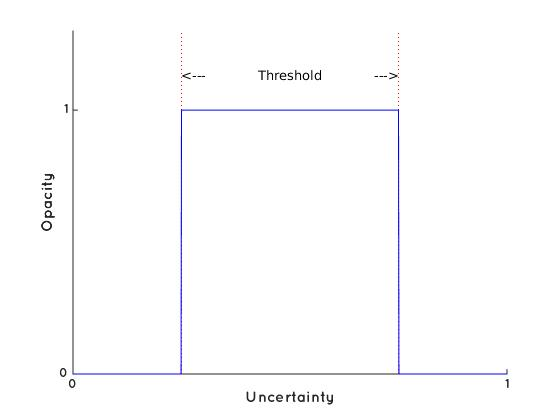
\includegraphics[width=\textwidth]{images/thresholding/thresholdvariation1.jpg}
    \caption{Variation 1}
    \label{fig:thresholdingvariation1}
  \end{subfigure}%
  ~ %add desired spacing between images, e. g. ~, \quad, \qquad, \hfill etc.
    %(or a blank line to force the subfigure onto a new line)
  \begin{subfigure}[b]{0.5\textwidth}
    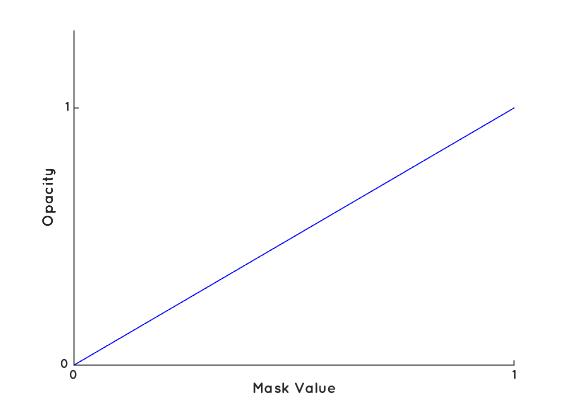
\includegraphics[width=\textwidth]{images/thresholding/thresholdvariation2.jpg}
    \caption{Variation 2}
    \label{fig:thresholdingvariation2}
  \end{subfigure}
  \caption{Opacity Transfer Functions. Opacity of 0 is transparent, 1 is opaque.}\label{fig:thresholdingoverview}
\end{figure}

An issue found with variation 1 was that the renderer still draws the edge of the uncertainty, even though it had previously been removed by erosion. This is due to the renderer using linear interpolation to take samples along each ray fired into the volume. Figure \ref{fig:thresholdingvariation1problem} illustrates the problem - the background has uncertainty 0.0, and the object has uncertainty $~$0.6. Points interpolated between the two will lie in the range 0.0-0.6 and so we find values of uncertainty that don't actually exist in the object.

\begin{figure}[h]
  \centering
  \begin{subfigure}[b]{0.5\textwidth}
    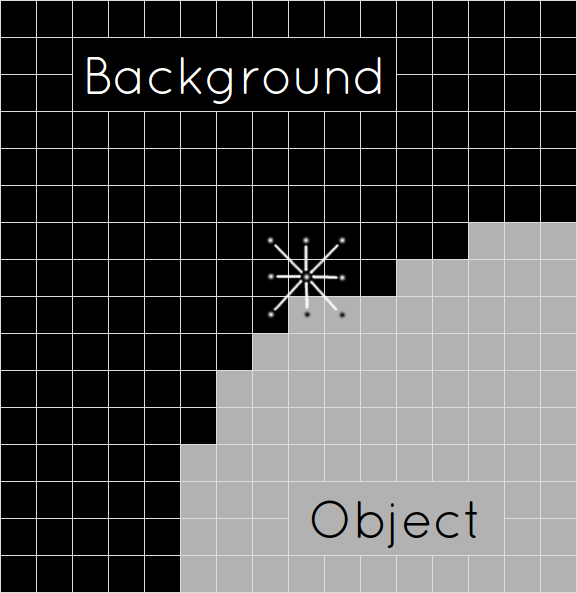
\includegraphics[width=\textwidth]{images/thresholding/thresholdvariation1example.png}
    \caption{Simplified View}
    \label{fig:thresholdingvariation1example}
  \end{subfigure}%
  ~ %add desired spacing between images, e. g. ~, \quad, \qquad, \hfill etc.
    %(or a blank line to force the subfigure onto a new line)
  \begin{subfigure}[b]{0.5\textwidth}
    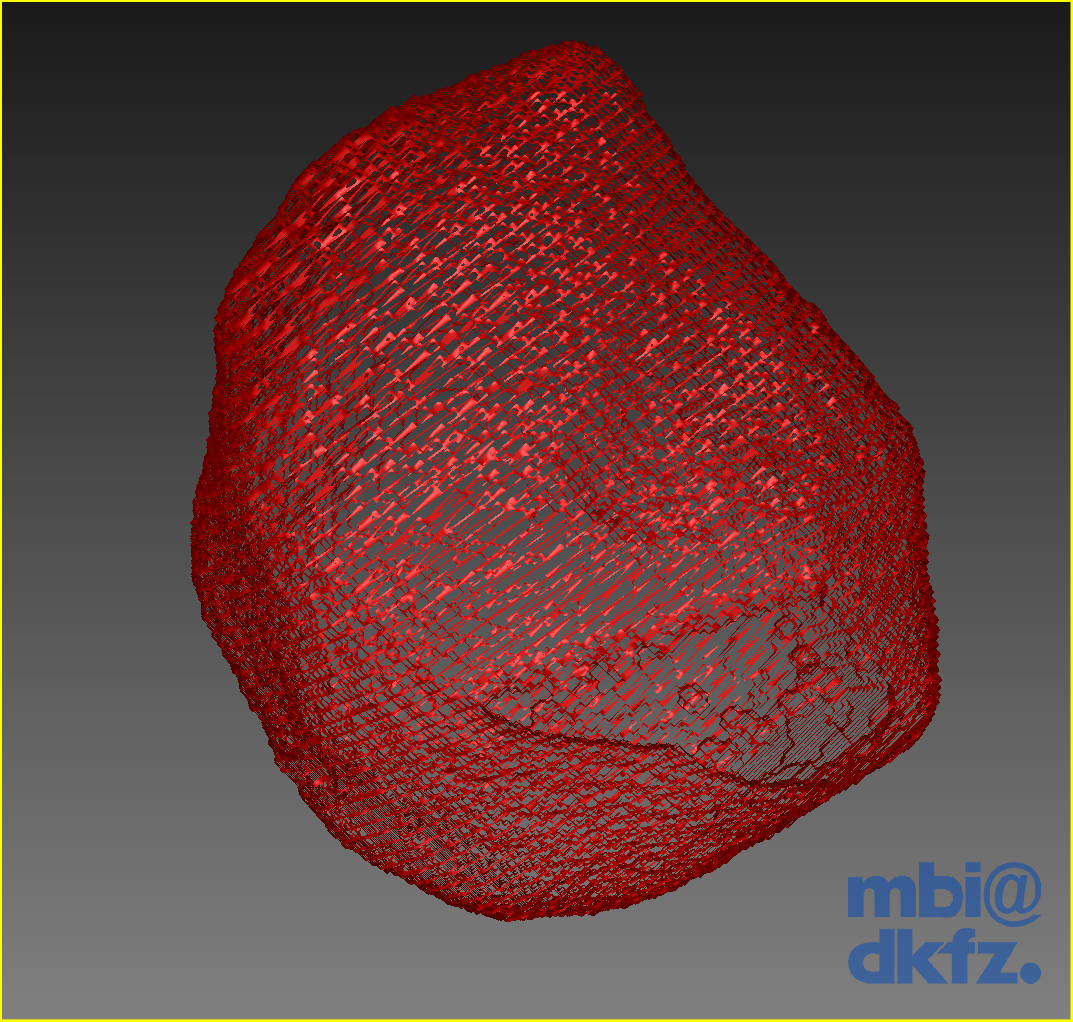
\includegraphics[width=\textwidth]{images/thresholding/thresholdvariation1problem.png}
    \caption{Edge Artefacts}
    \label{fig:thresholdingvariation1artefacts}
  \end{subfigure}
  \caption{Opacity Transfer Functions. Opacity of 0 is transparent, 1 is opaque.}\label{fig:thresholdingvariation1problem}
\end{figure}

A solution to this problem is to use a gradient transfer function which allows the change in uncertainty to influence the transparency. Rapid changes in uncertainty can therefore be treated as noise and ignored. The cutoff can be adjusted to remove the entire edge but there is a tradeoff as some genuine regions of uncertainty can also be filteredout. Figure \ref{fig:thresholdingvariationfix} shows the transfer function and the effect of tweaking the threshold.

\begin{figure}[H]
  \centering
  \begin{subfigure}[b]{0.5\textwidth}
    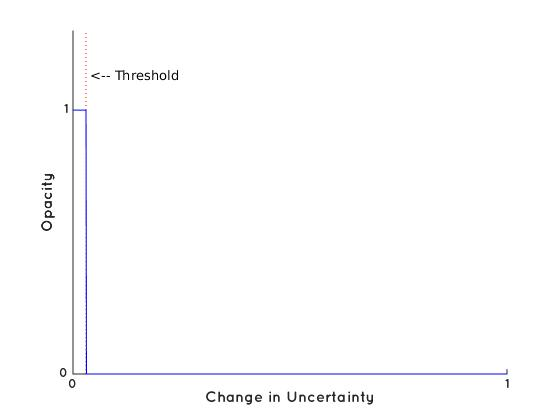
\includegraphics[width=\textwidth]{images/thresholding/thresholdvariation1fix.jpg}
    \caption{Gradient Transfer Function}
    \label{fig:thresholdingvariation1example}
  \end{subfigure}%
  ~ %add desired spacing between images, e. g. ~, \quad, \qquad, \hfill etc.
    %(or a blank line to force the subfigure onto a new line)
  \begin{subfigure}[b]{0.5\textwidth}
    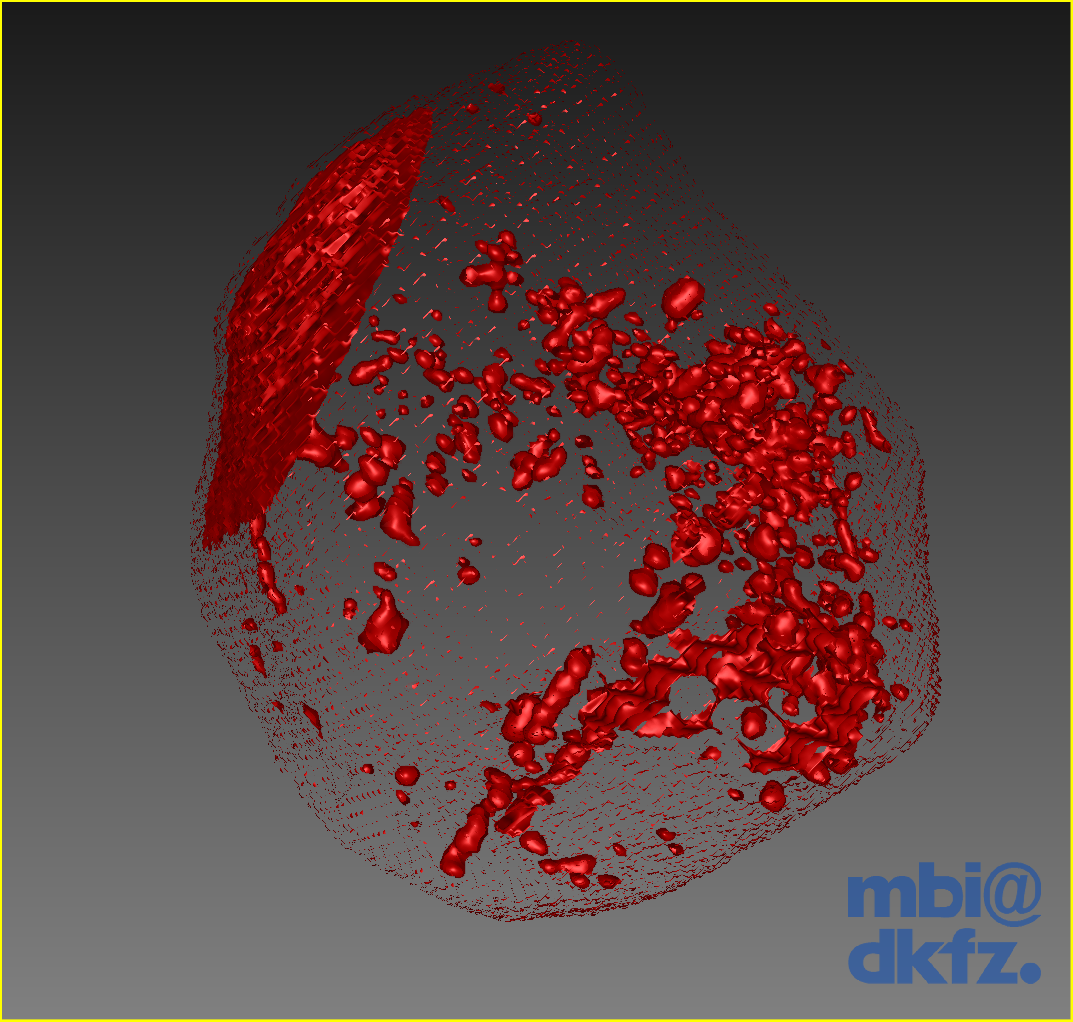
\includegraphics[width=\textwidth]{images/thresholding/thresholdvariation1threshold1.png}
    \caption{Threshold 0.05}
    \label{fig:thresholdingvariation1threshold1}
  \end{subfigure}
  ~%add desired spacing between images, e. g. ~, \quad, \qquad, \hfill etc.
    %(or a blank line to force the subfigure onto a new line)
  \begin{subfigure}[b]{0.5\textwidth}
    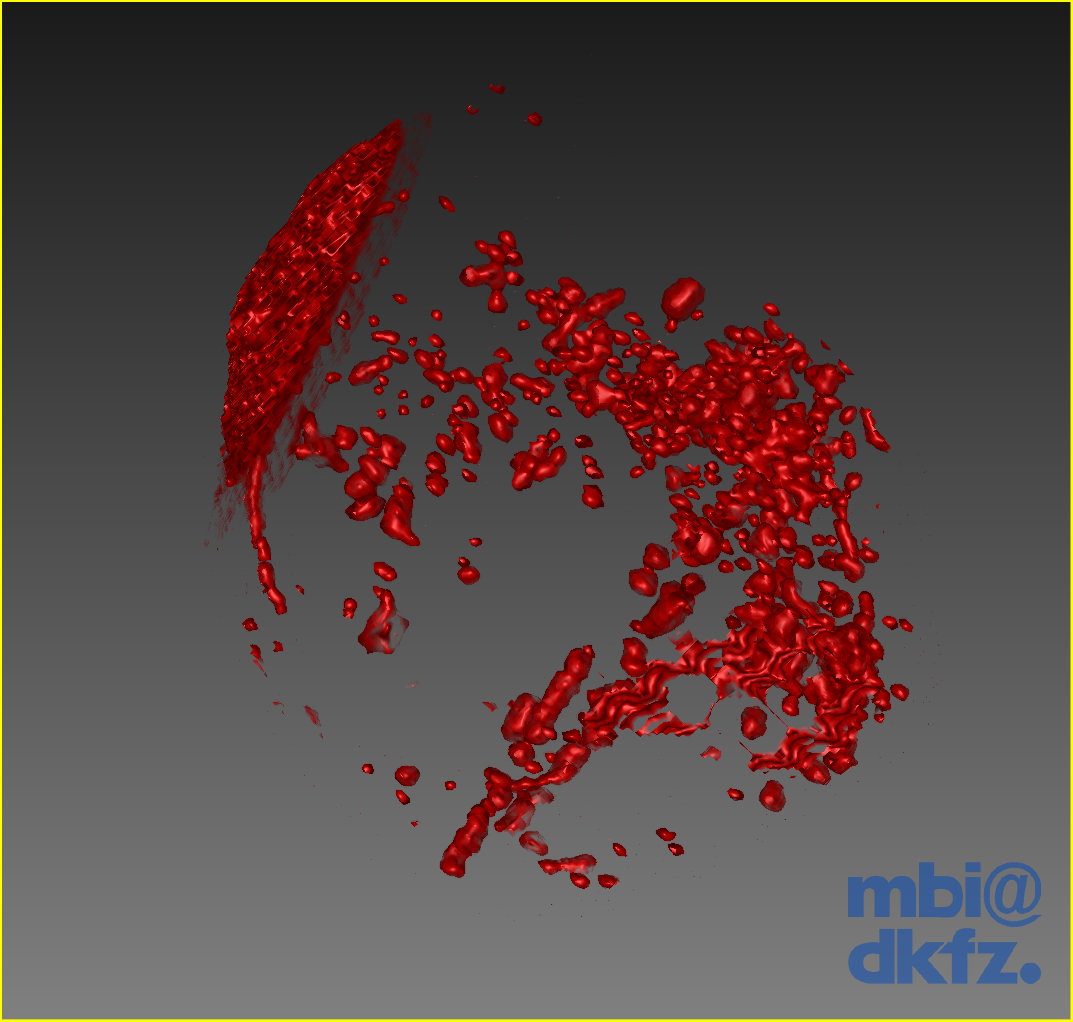
\includegraphics[width=\textwidth]{images/thresholding/thresholdvariation1threshold2.png}
    \caption{Threshold 0.02}
    \label{fig:thresholdingvariation1threshold2}  
  \end{subfigure}%
  ~ %add desired spacing between images, e. g. ~, \quad, \qquad, \hfill etc.
    %(or a blank line to force the subfigure onto a new line)
  \begin{subfigure}[b]{0.5\textwidth}
    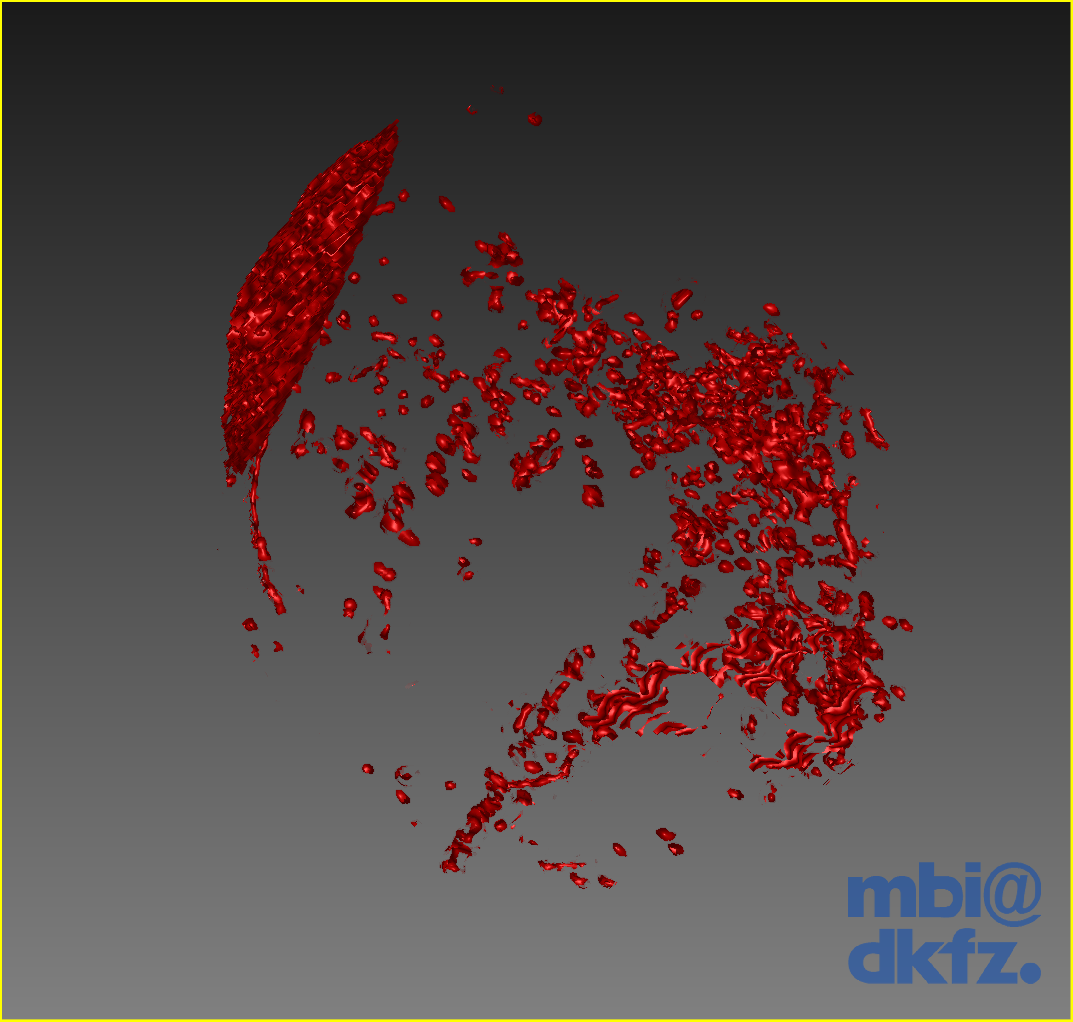
\includegraphics[width=\textwidth]{images/thresholding/thresholdvariation1threshold3.png}
    \caption{Threshold 0.01}
    \label{fig:thresholdingvariation1threshold3}  
  \end{subfigure}  
  \caption{Reducing the threshold removes the edge but removes some uncertainty.}\label{fig:thresholdingvariationfix}
\end{figure}

Although tweaking the threshold can remove edge artefact variation 2 was found not to exhibit these problems and so this implementation was used in the evaluation of the prototype.

\newpage
\subsection*{Results}
Here are the results that are achieved with the test uncertainties (see section \ref{section:testuncertainties}).

\begin{figure}[H]
  \centering
  \begin{subfigure}[b]{0.32\textwidth}
    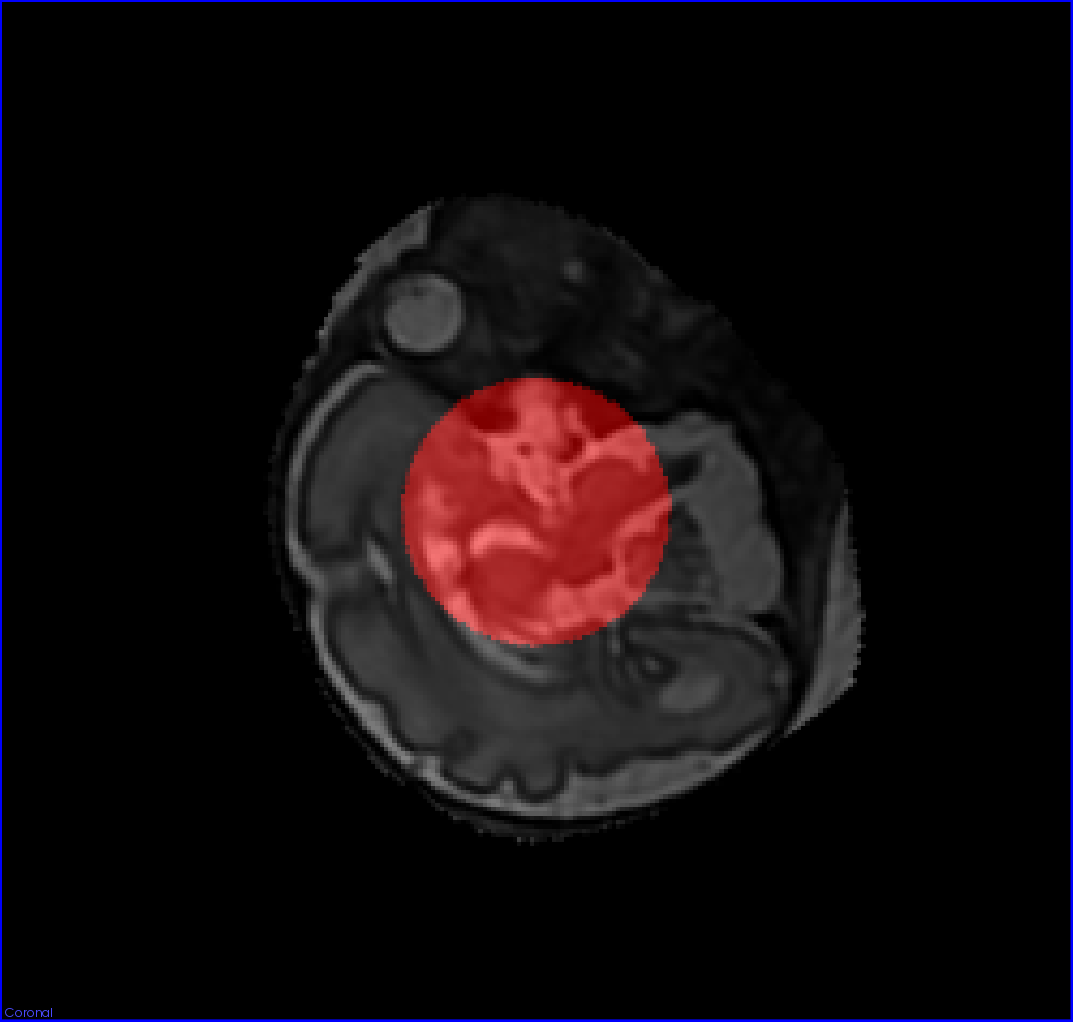
\includegraphics[width=\textwidth]{images/thresholding/results/sphere_2d.png}
    \caption{Sphere in 2D}
    \label{fig:thresholdingresultssphere2d}
  \end{subfigure}%
  ~ %add desired spacing between images, e. g. ~, \quad, \qquad, \hfill etc.
    %(or a blank line to force the subfigure onto a new line)
  \begin{subfigure}[b]{0.32\textwidth}
    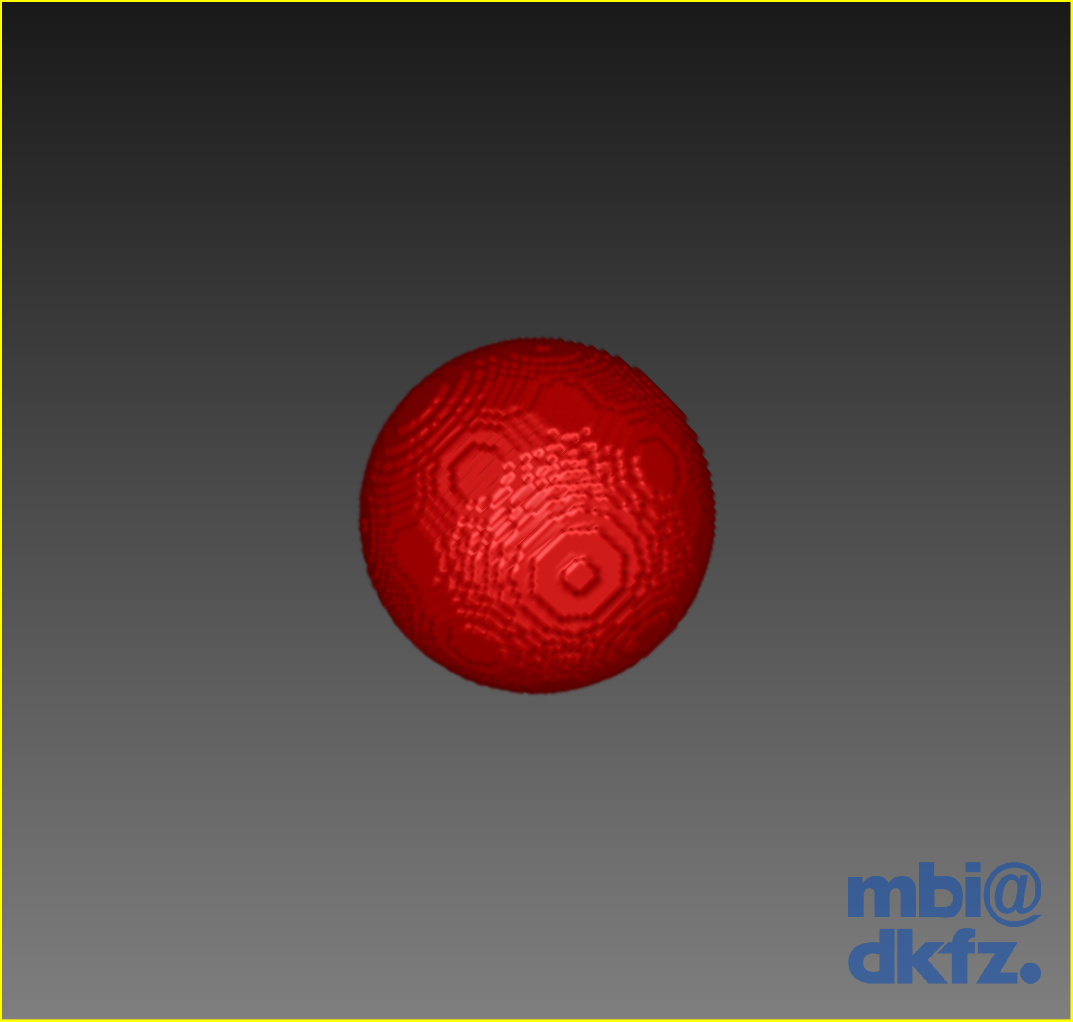
\includegraphics[width=\textwidth]{images/thresholding/results/sphere_3d.png}
    \caption{Sphere in 3D}
    \label{fig:thresholdingresultssphere3d}
  \end{subfigure}
  ~ %add desired spacing between images, e. g. ~, \quad, \qquad, \hfill etc.
    %(or a blank line to force the subfigure onto a new line)
  \begin{subfigure}[b]{0.32\textwidth}
    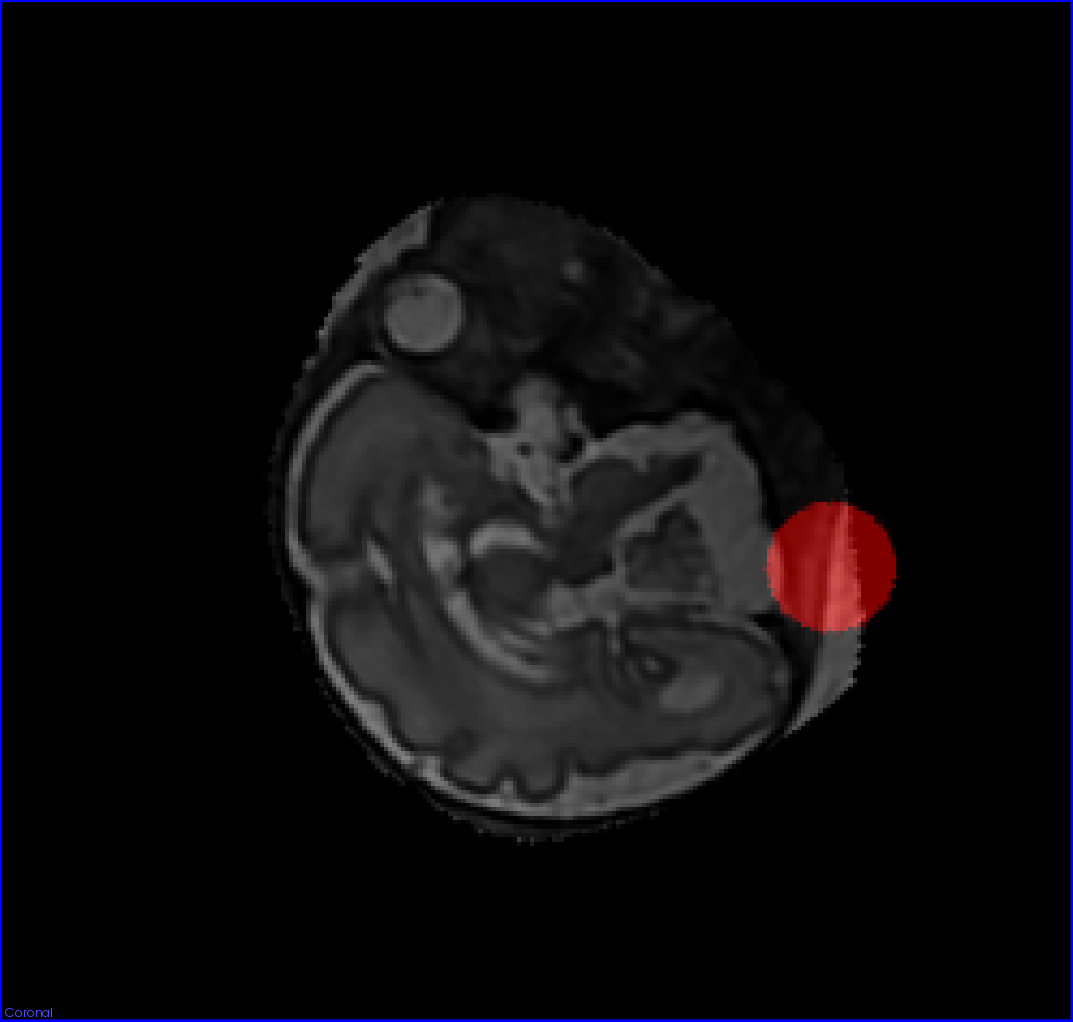
\includegraphics[width=\textwidth]{images/thresholding/results/sphere_corner_2d.png}
    \caption{Sphere in Corner in 2D}
    \label{fig:thresholdingresultsspherecorner2d}
  \end{subfigure}%
  ~ %add desired spacing between images, e. g. ~, \quad, \qquad, \hfill etc.
    %(or a blank line to force the subfigure onto a new line)
  \begin{subfigure}[b]{0.32\textwidth}
    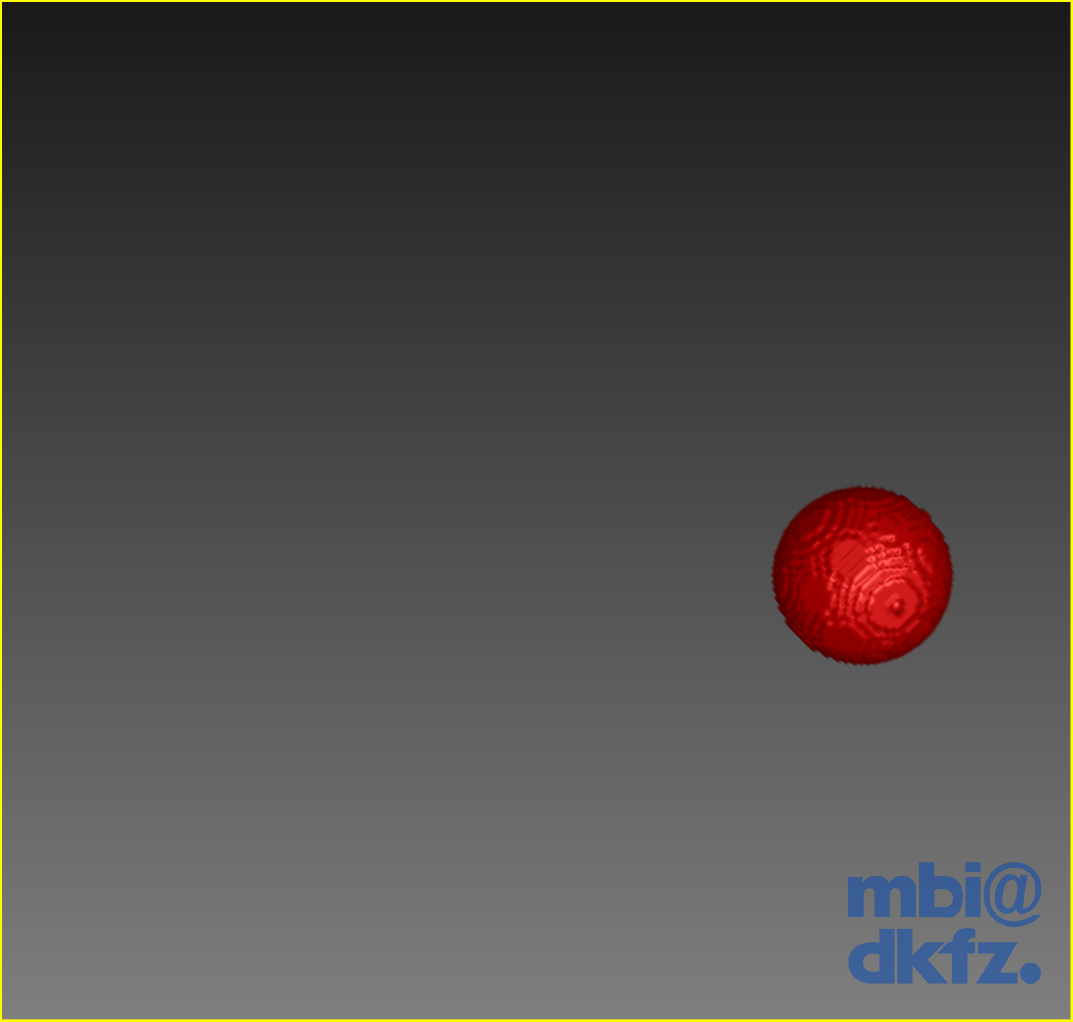
\includegraphics[width=\textwidth]{images/thresholding/results/sphere_corner_3d.png}
    \caption{Sphere in Corner in 3D}
    \label{fig:thresholdingresultsspherecorner3d}
  \end{subfigure}
  ~ %add desired spacing between images, e. g. ~, \quad, \qquad, \hfill etc.
    %(or a blank line to force the subfigure onto a new line)
  \begin{subfigure}[b]{0.32\textwidth}
    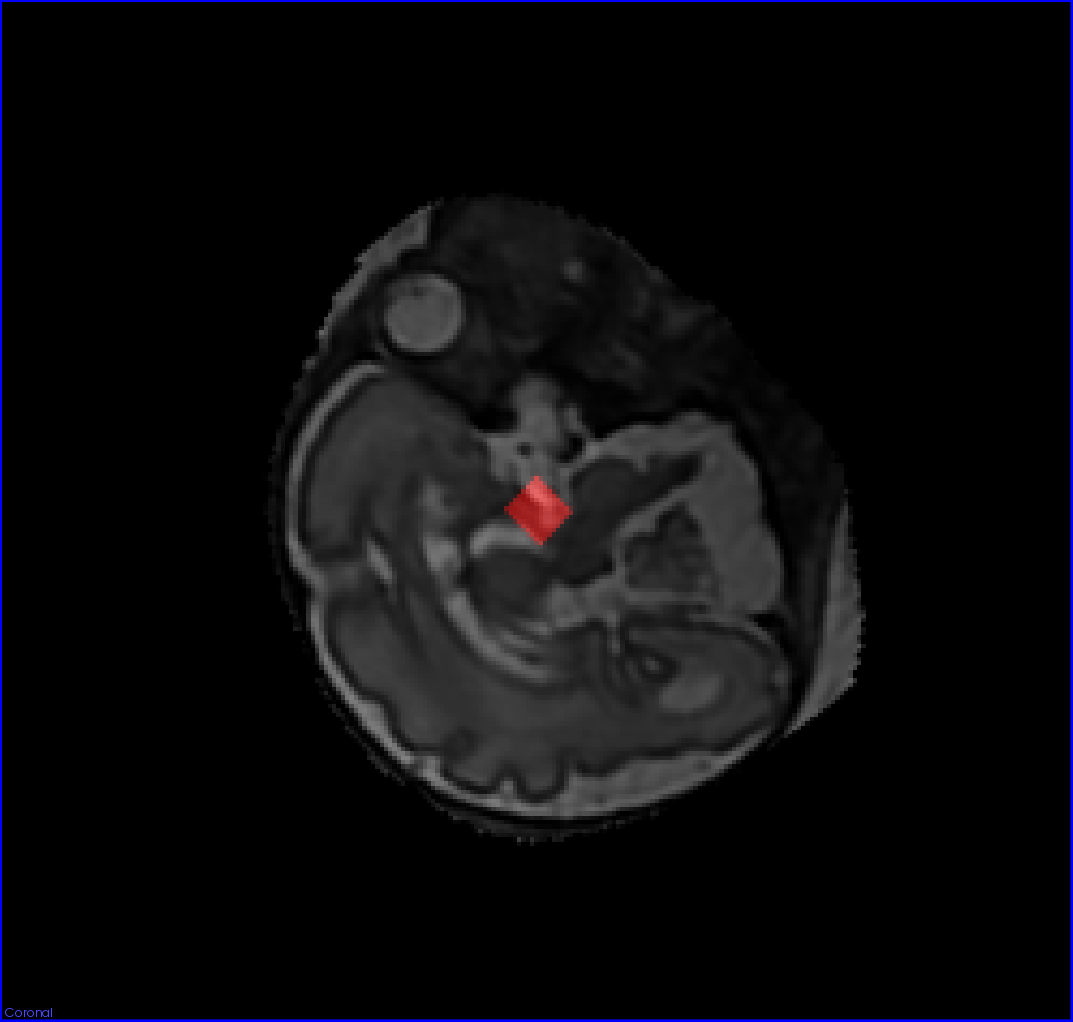
\includegraphics[width=\textwidth]{images/thresholding/results/cube_2d.png}
    \caption{Cube in 2D}
    \label{fig:thresholdingresultscube2d}
  \end{subfigure}%
  ~ %add desired spacing between images, e. g. ~, \quad, \qquad, \hfill etc.
    %(or a blank line to force the subfigure onto a new line)
  \begin{subfigure}[b]{0.32\textwidth}
    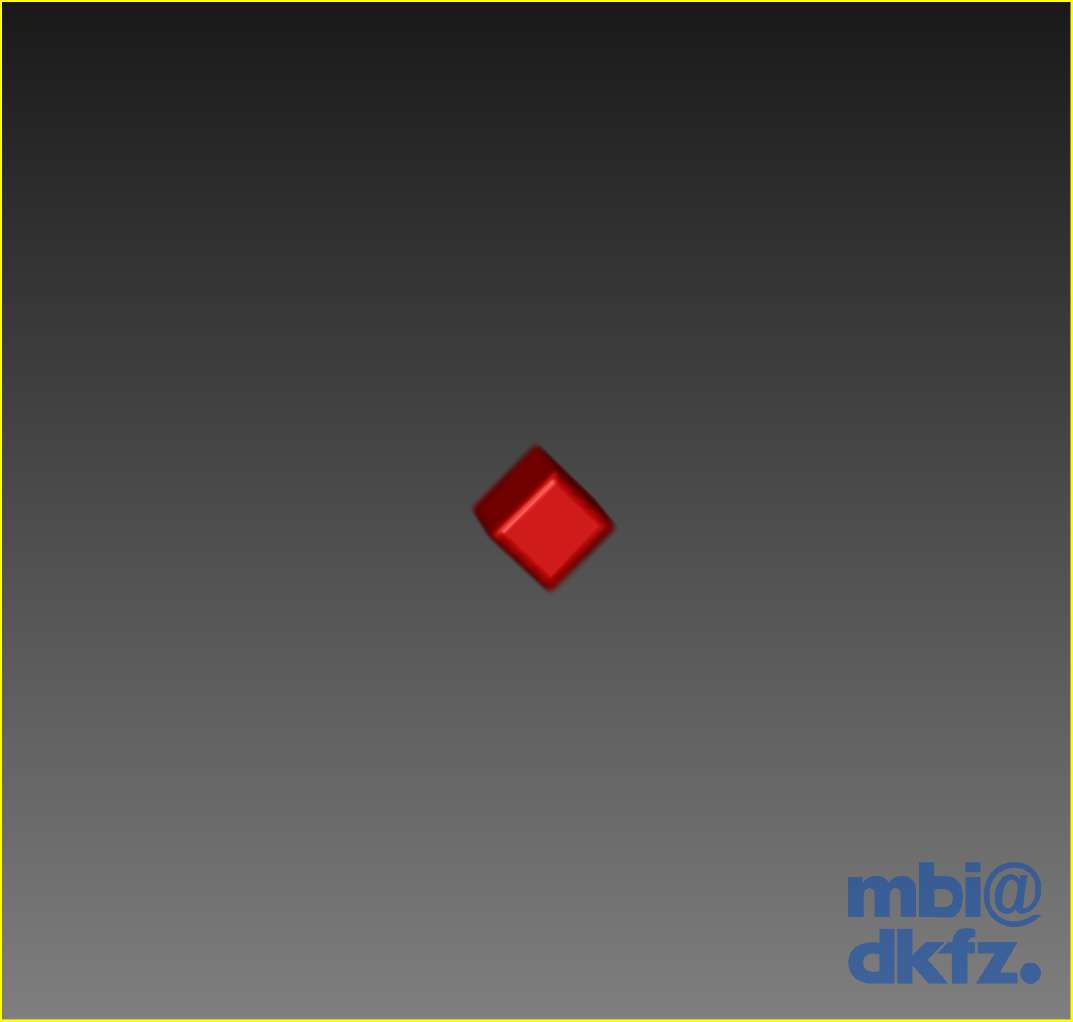
\includegraphics[width=\textwidth]{images/thresholding/results/cube_3d.png}
    \caption{Cube in 3D}
    \label{fig:thresholdingresultscube3d}
  \end{subfigure}
  ~ %add desired spacing between images, e. g. ~, \quad, \qquad, \hfill etc.
    %(or a blank line to force the subfigure onto a new line)
  \begin{subfigure}[b]{0.32\textwidth}
    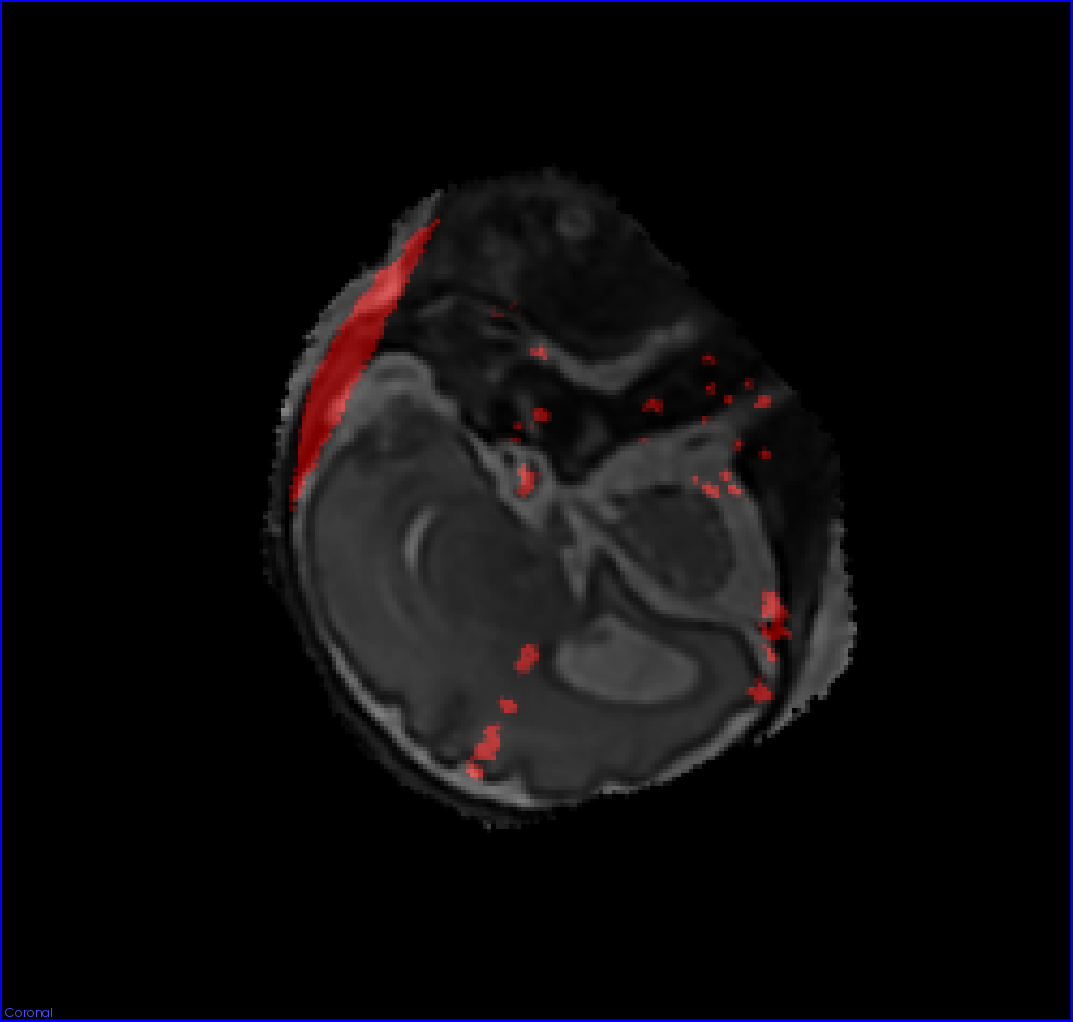
\includegraphics[width=\textwidth]{images/thresholding/results/scan_2d.png}
    \caption{Scan in 2D}
    \label{fig:thresholdingresultsscan2d}
  \end{subfigure}%
  ~ %add desired spacing between images, e. g. ~, \quad, \qquad, \hfill etc.
    %(or a blank line to force the subfigure onto a new line)
  \begin{subfigure}[b]{0.32\textwidth}
    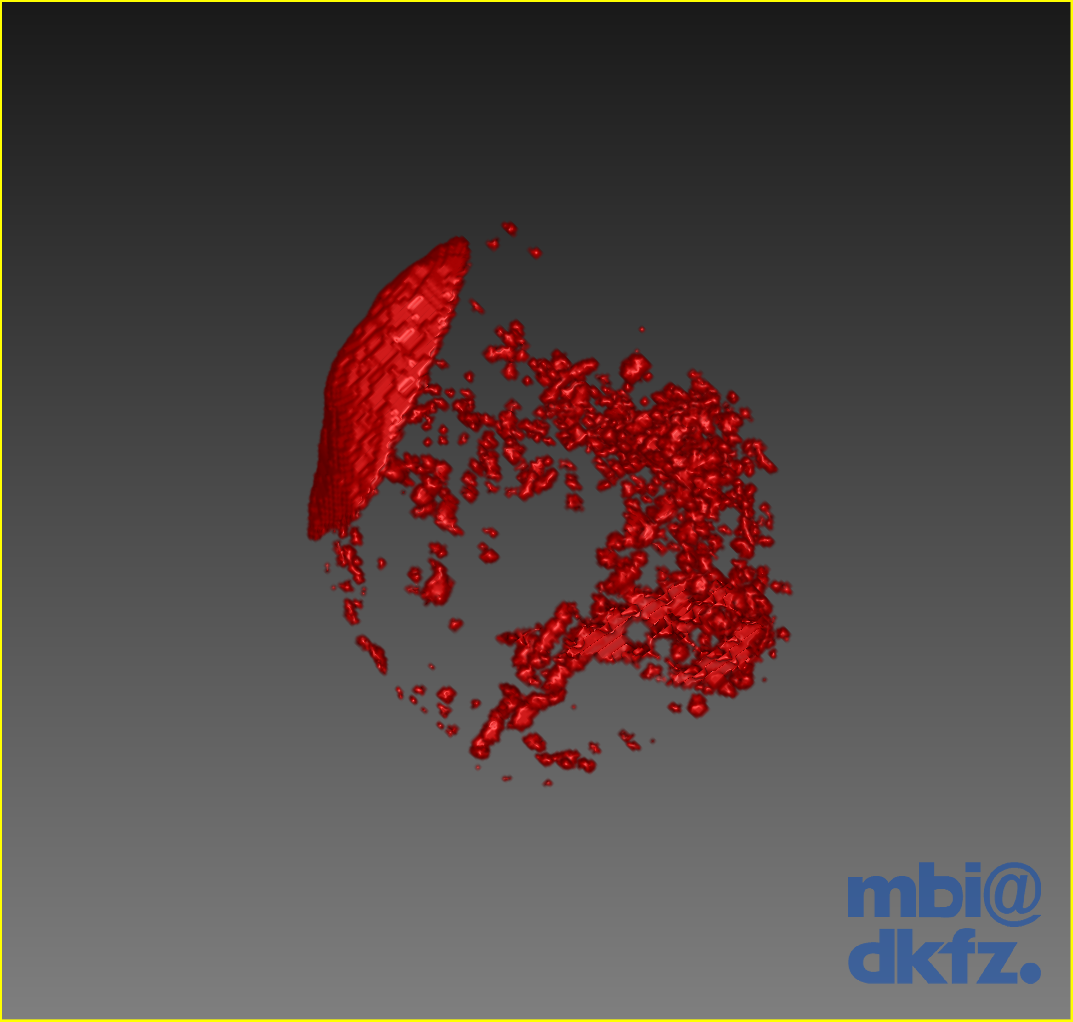
\includegraphics[width=\textwidth]{images/thresholding/results/scan_3d.png}
    \caption{Scan in 3D}
    \label{fig:thresholdingresultsscan3d}
  \end{subfigure}
  % \caption{Opacity Transfer Functions. Opacity of 0 is transparent, 1 is opaque.}\label{fig:thresholdingvariation1problem}
\end{figure}

\newpage
\section{Uncertainty Surface}\label{section:uncertaintysurface}
The idea behind the uncertainty surface is to project the uncertainty (a 3D volume) onto a surface (effectively 2D) to give an overview of the uncertainty hotspots. Two versions have been implemented; the first maps the uncertainty to a sphere and the second maps the uncertainty to a surface representation of the organ being scanned. The uncertainty sphere is a generic visualization that can be applied to any scan, whereas the second requires a surface representation of the organ in question.

\subsection*{Sphere}
Two ways of mapping the uncertainty to the surfaces have been trialled. Originally the uncertainty was mapped to a texture which could then be applied to a surface. 

Figure \ref{fig:uncertaintytexture} shows such a texture and the result when viewed on a sphere. To generate the uncertainty at each pixel the position (x, y) is first converted to spherical coordinates ($\theta$, $\phi$). These are then converted to a point (x', y', z') on a sphere of unit radius. The uncertainty at pixel (x, y) is then calculated by firing a ray from the center of the volume outwards, in direction (x', y', z') and accumulating uncertainty as it goes (see volume rendering section \\ref{background:volumerendering}).

\begin{figure}[H]
  \centering
  \begin{subfigure}[b]{0.5\textwidth}
    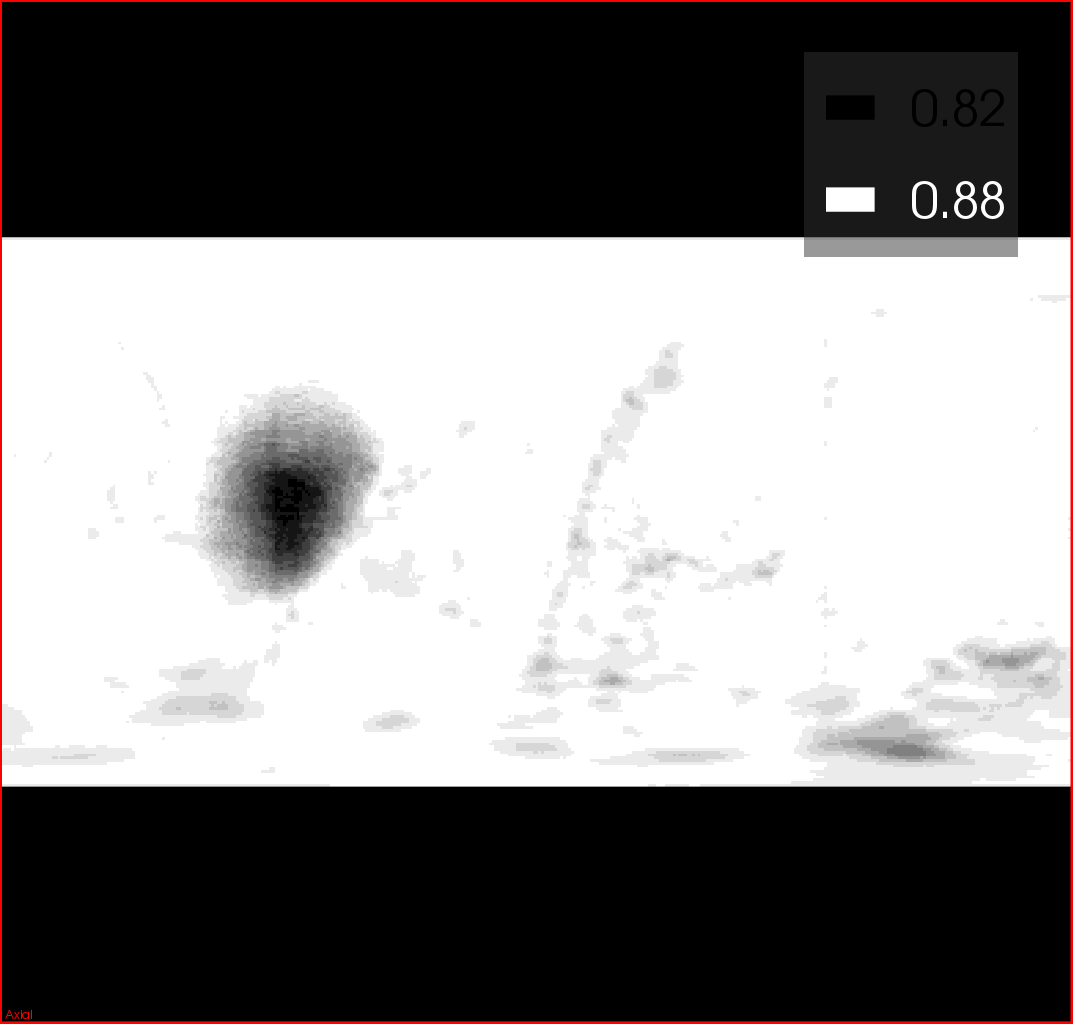
\includegraphics[width=\textwidth]{images/surface/texture_texture.png}
    \caption{Uncertainty Texture}
    \label{fig:texturetexture}
  \end{subfigure}%
  ~ %add desired spacing between images, e. g. ~, \quad, \qquad, \hfill etc.
    %(or a blank line to force the subfigure onto a new line)
  \begin{subfigure}[b]{0.5\textwidth}
    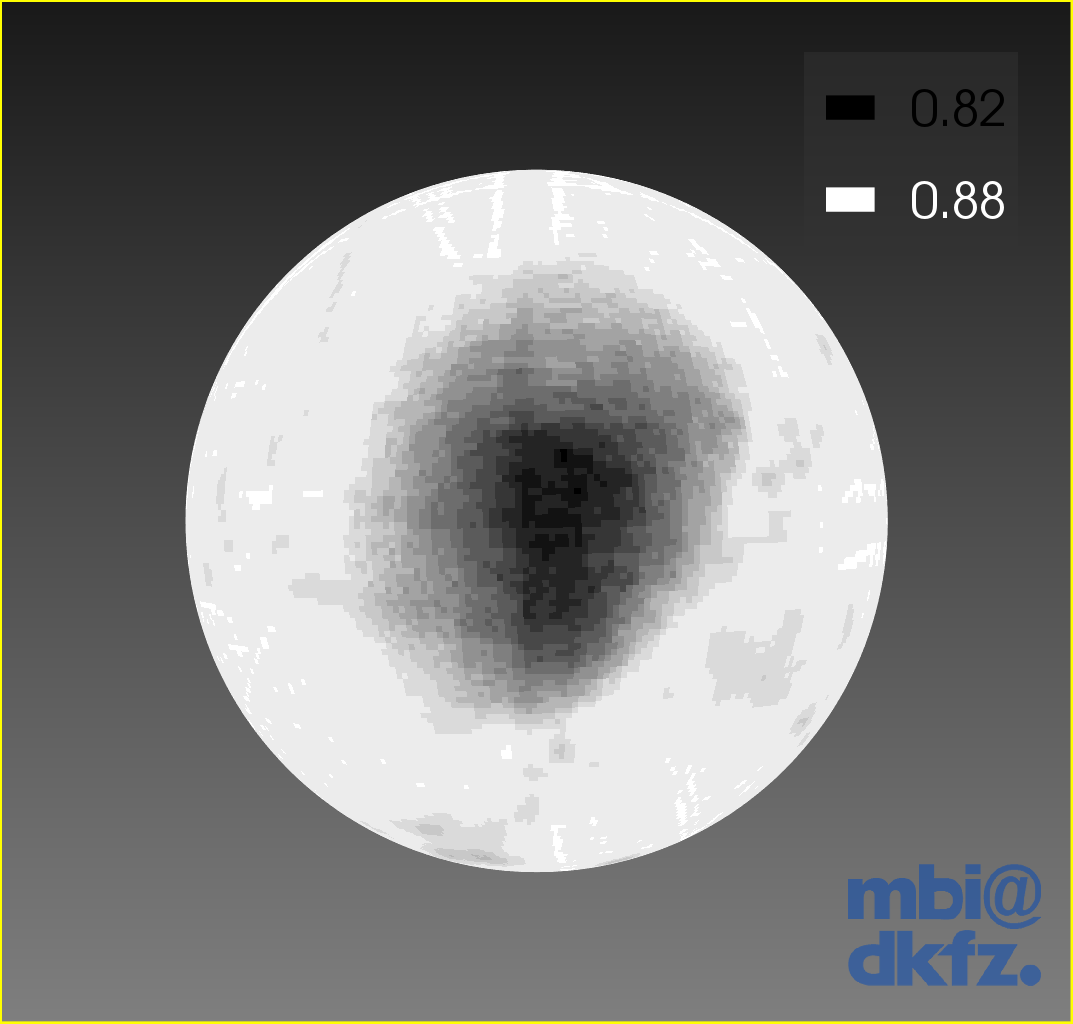
\includegraphics[width=\textwidth]{images/surface/texture_sphere.png}
    \caption{Mapped to Sphere}
    \label{fig:texturesphere}
  \end{subfigure}
  \caption{Mapping a texture to a sphere.}\label{fig:uncertaintytexture}
\end{figure}

This technique has a number of issues. Firstly, it looks quite blocky unless the resolution is set very high. Secondly, due to the conversion to spherical coordinates parts of the sphere are less well represented - as an extreme the top row of pixels on the texture all correspond to the top point on the sphere. Finally this technique does not translate very well when trying to map to arbitrary surfaces that are not as regular as a sphere.

Another approach was then trialled. In MITK it is possible to store a colour at each point on a surface and use the colours at each point to interpolate values all over the surface. This effectively removes the need for the texture, as each point on the surface can be set directly in turn.

This process begins by generating a surface representation of a sphere - the resolution of this model can be changed to alter the number of points used to approximate the sphere.

Then each point on the sphere is registered to a start point to begin sampling in the volume (volume intersection in figure). The normal of the point on the sphere is then used as a direction to sample in. The start of the genuine uncertainty is then found by following the sampling direction until the value is not background (uncertainty intersection in figure). Figure \ref{fig:surface_sampling_example} illustrates this process.

\begin{figure}[H]
  \centering
  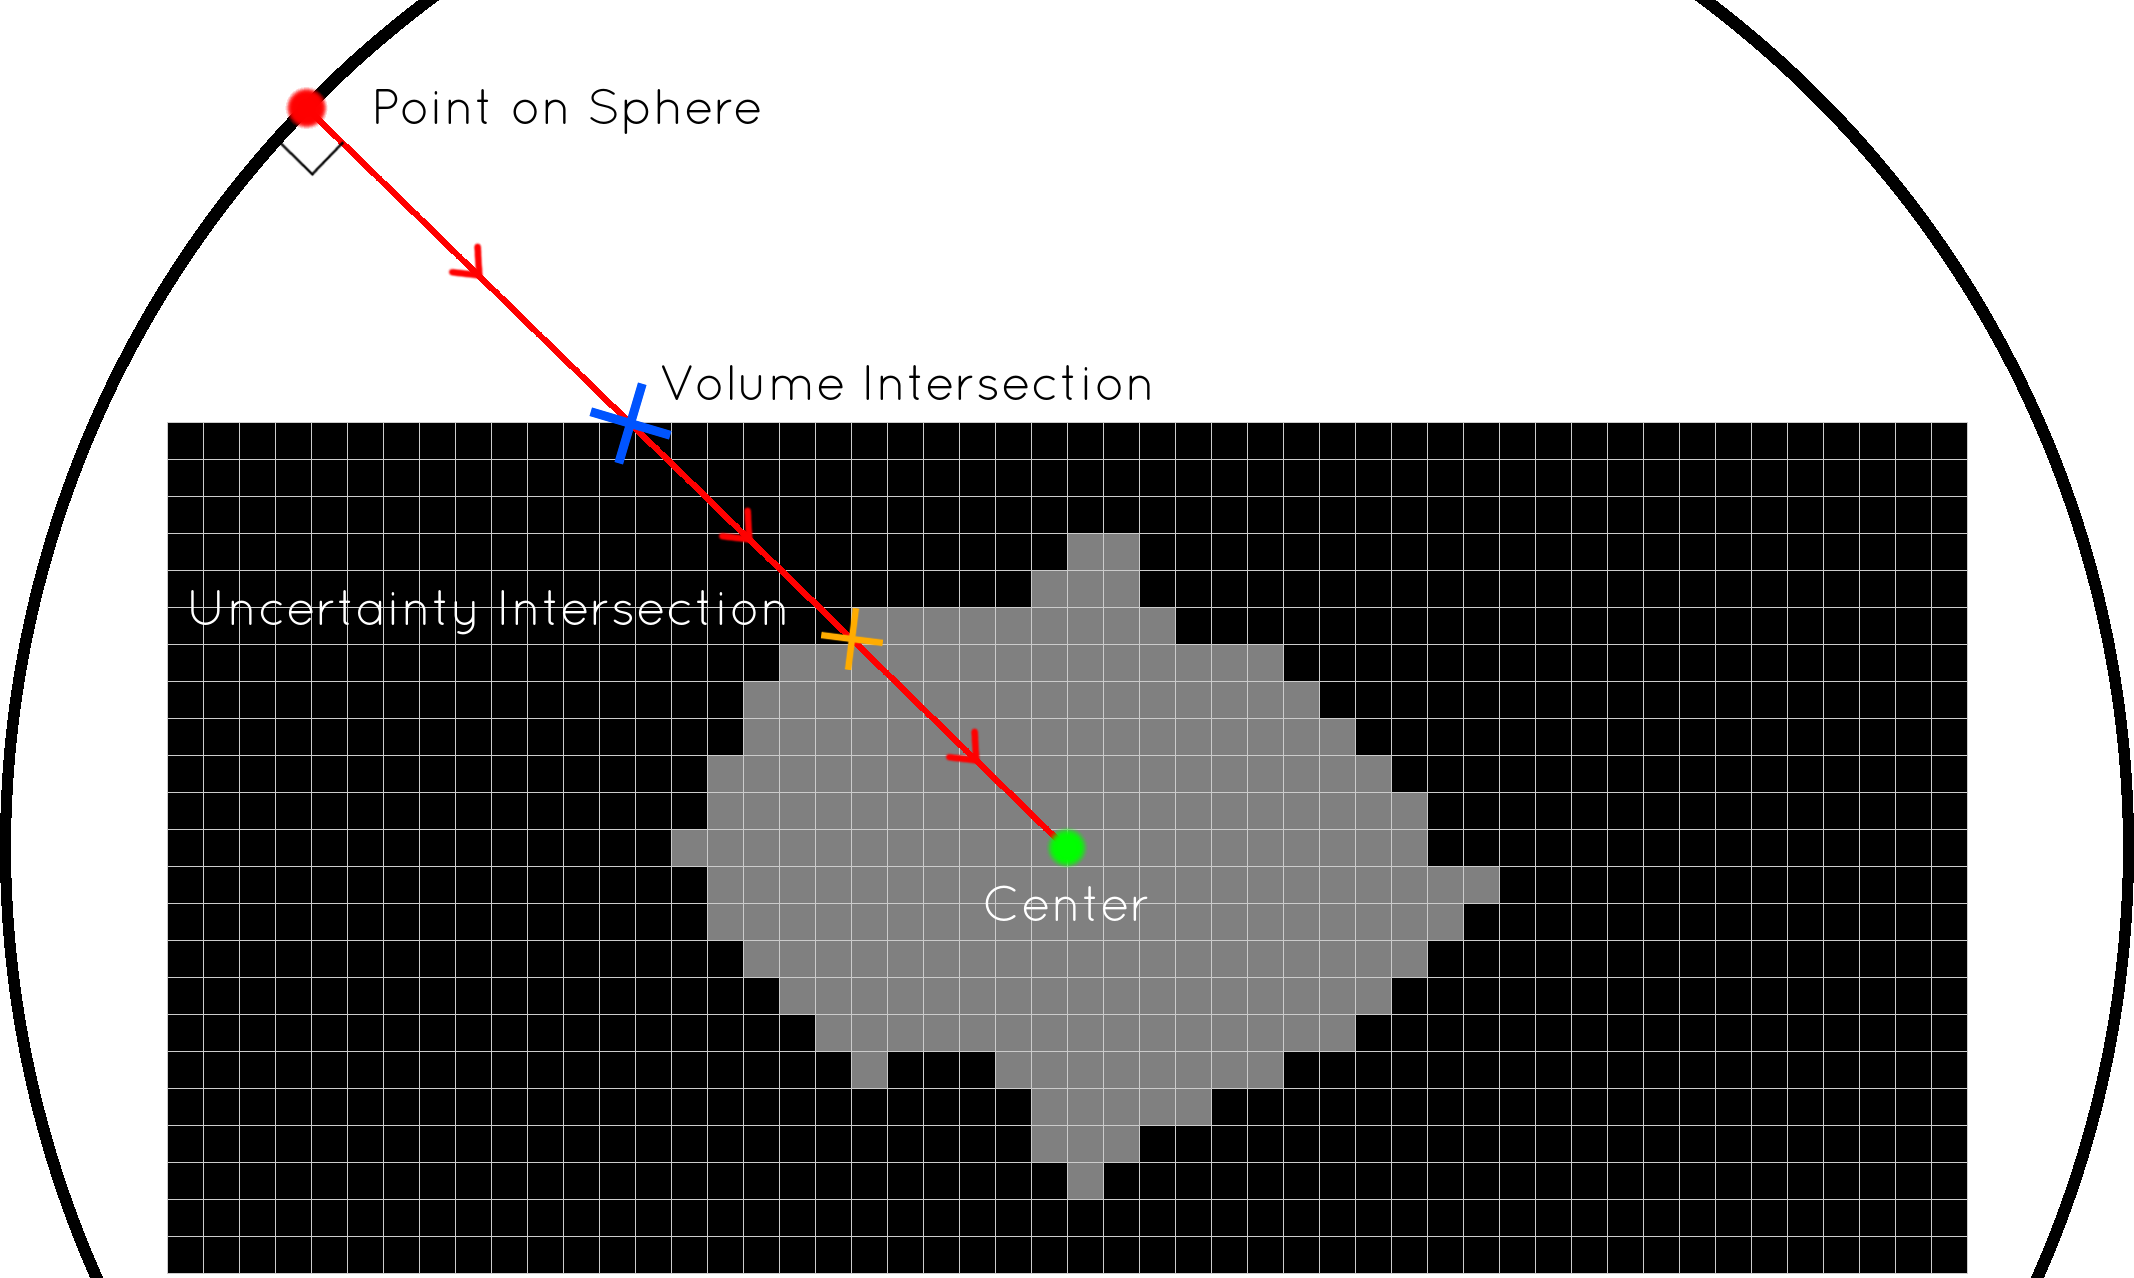
\includegraphics[width=\textwidth]{images/surface/sampling_example.png}
  \caption{Sampling Overview}\label{fig:surface_sampling_example}
\end{figure}

A tortoise and hare algorithm is then used to be able to vary how far into the volume the sampling goes. The tortoise moves through the uncertainty accumulating samples whilst the hare shoots off trying to find the edge. When the hare does find the edge the sampling stops. If the hare travels at the same speed as the tortoise then the entire object is sampled, if it travels at twice the speed of the tortoise then the sampling stops half the way through and so on. This is illustrated in figure \ref{fig:tortoiseandhareexample}.

\begin{figure}[H]
  \centering
  \begin{subfigure}[b]{0.32\textwidth}
    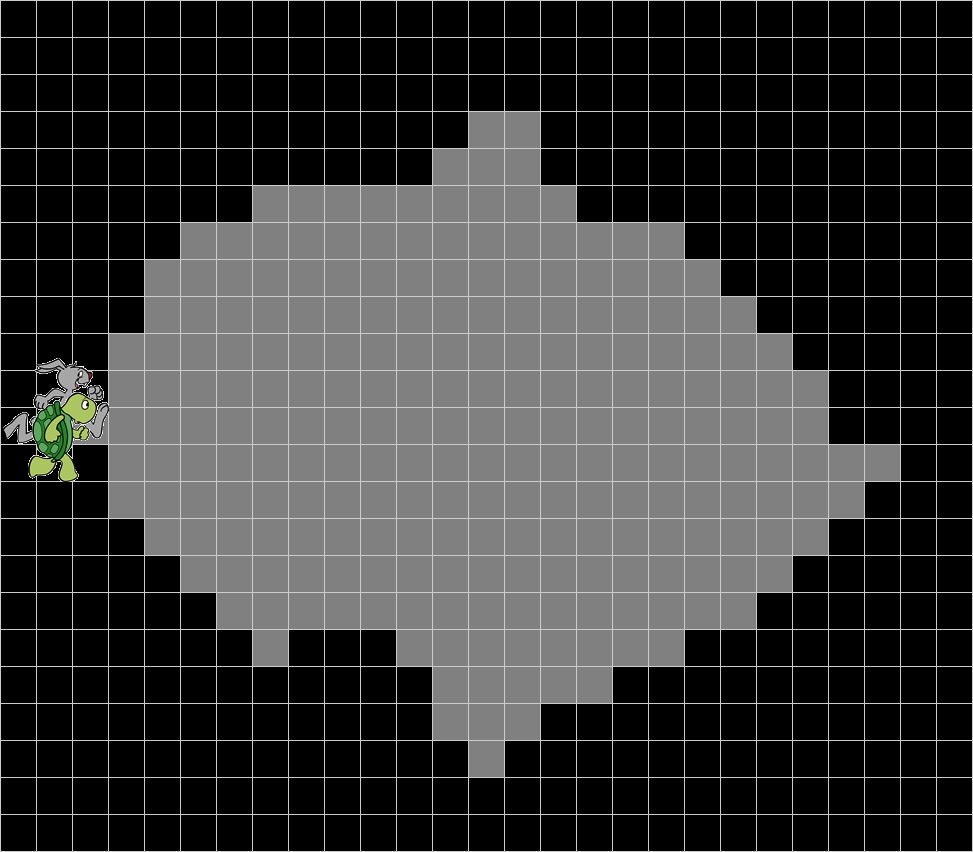
\includegraphics[width=\textwidth]{images/surface/tortoise_and_hare_1.png}
    \caption{Start}
    \label{fig:tortoiseandhare1}
  \end{subfigure}%
  ~ %add desired spacing between images, e. g. ~, \quad, \qquad, \hfill etc.
    %(or a blank line to force the subfigure onto a new line)
  \begin{subfigure}[b]{0.32\textwidth}
    \includegraphics[width=\textwidth]{images/surface/tortoise_and_hare_2.png}
    \caption{...}
    \label{fig:tortoiseandhare2}
  \end{subfigure}%
  ~ %add desired spacing between images, e. g. ~, \quad, \qquad, \hfill etc.
    %(or a blank line to force the subfigure onto a new line)
  \begin{subfigure}[b]{0.32\textwidth}
    \includegraphics[width=\textwidth]{images/surface/tortoise_and_hare_3.png}
    \caption{End}
    \label{fig:tortoiseandhare3}  
  \end{subfigure}
  \caption{Illustration of Tortoise and Hare Algorithm}\label{fig:tortoiseandhareexample}
\end{figure}

The accumulation that the tortoise does can also be customized. By default it will take the average of all of the samples it takes, but the best value and also the worst value along the ray can be extracted.

Once all of the points have been computed some scaling can be implemented to improve the contrast of the visualization. In many cases the average uncertainty will be roughly the same everywhere and if the range (0-1) is mapped to the entire colour range the values end up looking idential; to fix this the outputted colour range can be linearly mapped to make better use of the colours available.

\subsection*{Surface}

To map to a different surface model the procedure is largely the same. Again the first step is to generate the surface representation. Currently this is done using the mask supplied in the reconstruction step - applying surface extraction and mesh decimation (see section \ref{background:surfaceextraction}) to create a rough surface representation.

The registration step in this case is trivial as the mask uses the same coordinate system as the uncertainty volume. The normal at the surface can then be used, as before, and scaling similarly applied.

\newpage
\subsection*{Results}
Scaling was found to significantly increase the contrast of the visualization. The legend shows the scaling applied in each case.

\begin{figure}[H]
  \centering
  \begin{subfigure}[b]{0.25\textwidth}
    \includegraphics[width=\textwidth]{images/surface/sphere_no_scaling.png}
    \caption*{Sphere\\(No Scaling)}
    \label{fig:surfacespherenoscaling}
  \end{subfigure}%
    %add desired spacing between images, e. g. ~, \quad, \qquad, \hfill etc.
    %(or a blank line to force the subfigure onto a new line)
  \begin{subfigure}[b]{0.25\textwidth}
    \includegraphics[width=\textwidth]{images/surface/sphere_scaling.png}
    \caption*{Sphere\\(Linear)}
    \label{fig:surfacespherescaling}
  \end{subfigure}%
    %add desired spacing between images, e. g. ~, \quad, \qquad, \hfill etc.
    %(or a blank line to force the subfigure onto a new line)
  \begin{subfigure}[b]{0.25\textwidth}
    \includegraphics[width=\textwidth]{images/surface/surface_no_scaling.png}
    \caption*{Surface\\(No Scaling)}
    \label{fig:surfacesurfacenoscaling}
  \end{subfigure}%
    %add desired spacing between images, e. g. ~, \quad, \qquad, \hfill etc.
    %(or a blank line to force the subfigure onto a new line)
  \begin{subfigure}[b]{0.25\textwidth}
    \includegraphics[width=\textwidth]{images/surface/surface_scaling.png}
    \caption*{Sphere\\(Linear)}
    \label{fig:surfacesurfacescaling}
  \end{subfigure}
  \caption{The effect of linear mapping.}\label{fig:surfacescaling}
\end{figure}

The surface representation difficult to interpret by looking at a single image in a report. Figure \ref{fig:surface180} illustrates various angles. In practice all of these visualizations can be rotated and zoomed.

\begin{figure}[h]
  \centering
  \begin{subfigure}[b]{0.20\textwidth}
    \includegraphics[width=\textwidth]{images/surface/surface_180_1.png}
    \caption*{Left}
    \label{fig:erosion0}
  \end{subfigure}%
    %add desired spacing between images, e. g. ~, \quad, \qquad, \hfill etc.
    %(or a blank line to force the subfigure onto a new line)
  \begin{subfigure}[b]{0.20\textwidth}
    \includegraphics[width=\textwidth]{images/surface/surface_180_2.png}
    \caption*{Front Left}
    \label{fig:erosion1}
  \end{subfigure}%
    %add desired spacing between images, e. g. ~, \quad, \qquad, \hfill etc.
    %(or a blank line to force the subfigure onto a new line)
  \begin{subfigure}[b]{0.20\textwidth}
    \includegraphics[width=\textwidth]{images/surface/surface_180_3.png}
    \caption*{Front}
    \label{fig:erosion2}
  \end{subfigure}%
    %add desired spacing between images, e. g. ~, \quad, \qquad, \hfill etc.
    %(or a blank line to force the subfigure onto a new line)
  \begin{subfigure}[b]{0.20\textwidth}
    \includegraphics[width=\textwidth]{images/surface/surface_180_4.png}
    \caption*{Front Right}
    \label{fig:erosion3}
  \end{subfigure}%
    %add desired spacing between images, e. g. ~, \quad, \qquad, \hfill etc.
    %(or a blank line to force the subfigure onto a new line)
  \begin{subfigure}[b]{0.20\textwidth}
    \includegraphics[width=\textwidth]{images/surface/surface_180_5.png}
    \caption*{Right}
    \label{fig:erosion3}
  \end{subfigure}
  \caption{Brain surface viewed from different directions.}\label{fig:surface180}
\end{figure}

The default behaviour of taking the average uncertainty along the ray does a good job of bringing out the uncertainty but switching to the worst brings severe values that would otherwise be outweighed by good values to the surface. Switching to the best value isolates only truly terrible areas.

\begin{figure}[H]
  \centering
  \begin{subfigure}[b]{0.32\textwidth}
    \includegraphics[width=\textwidth]{images/surface/sphere_average.png}
    \caption{Average}
    \label{fig:sphereaverage}
  \end{subfigure}%
  ~ %add desired spacing between images, e. g. ~, \quad, \qquad, \hfill etc.
    %(or a blank line to force the subfigure onto a new line)
  \begin{subfigure}[b]{0.32\textwidth}
    \includegraphics[width=\textwidth]{images/surface/sphere_worst.png}
    \caption{Worst}
    \label{fig:sphereworst}
  \end{subfigure}%
  ~ %add desired spacing between images, e. g. ~, \quad, \qquad, \hfill etc.
    %(or a blank line to force the subfigure onto a new line)
  \begin{subfigure}[b]{0.32\textwidth}
    \includegraphics[width=\textwidth]{images/surface/sphere_best.png}
    \caption{Best}
    \label{fig:spherebest}  
  \end{subfigure}
  ~ %add desired spacing between images, e. g. ~, \quad, \qquad, \hfill etc.
    %(or a blank line to force the subfigure onto a new line)  
  \begin{subfigure}[b]{0.32\textwidth}
    \includegraphics[width=\textwidth]{images/surface/surface_average.png}
    \caption{Average}
    \label{fig:surfaceaverage}
  \end{subfigure}%
  ~ %add desired spacing between images, e. g. ~, \quad, \qquad, \hfill etc.
    %(or a blank line to force the subfigure onto a new line)
  \begin{subfigure}[b]{0.32\textwidth}
    \includegraphics[width=\textwidth]{images/surface/surface_worst.png}
    \caption{Worst}
    \label{fig:surfaceworst}
  \end{subfigure}%
  ~ %add desired spacing between images, e. g. ~, \quad, \qquad, \hfill etc.
    %(or a blank line to force the subfigure onto a new line)
  \begin{subfigure}[b]{0.32\textwidth}
    \includegraphics[width=\textwidth]{images/surface/surface_best.png}
    \caption{Best}
    \label{fig:surfacebest}  
  \end{subfigure}  
  \caption{Comparison of Average/Best/Worst sampling.}\label{fig:surfaceaccumulator}
\end{figure}

The sample distance determines how far into the volume samples go. Currently there are two options available - half and full. These options are less applicable to the sphere as if it is set to full then opposite sides of the sphere give identical values. When applied to the surface the use of this option very much depends on the area of the body that is being scanned. The brain is a large, and for the most part (ignoring folds particularly) convex; in this respect it is similar to the sphere and the effect of sampling all the way through is much the same (see figure \ref{fig:surfacesampledistance}). You can notice that the average uncertainty gets better with full sampling as there are more good points to outweigh the bad.

\begin{figure}[H]
  \centering
  \begin{subfigure}[b]{0.5\textwidth}
    \includegraphics[width=\textwidth]{images/surface/surface_half.png}
    \caption{Half}
    \label{fig:surfacehalf}
  \end{subfigure}%
  ~ %add desired spacing between images, e. g. ~, \quad, \qquad, \hfill etc.
    %(or a blank line to force the subfigure onto a new line)
  \begin{subfigure}[b]{0.5\textwidth}
    \includegraphics[width=\textwidth]{images/surface/surface_full.png}
    \caption{Full}
    \label{fig:surfacefull}
  \end{subfigure}
  \caption{Comparing half and full distance sampling.}\label{fig:surfacesampledistance}
\end{figure}

Where this parameter may be more useful however is when dealing with smaller, more intricate objects, such as arteries. It would allow the uncertainty the entire cross section to be mapped to the surface which would give an overview of the uncertainty in that section at a glance, rather than having to rotate around it to get the full picture.

\newpage
\section{Next Scan Plane}\label{section:nextscanplane}
The idea behind this visualization is based on some previous research\cite{uncertaintysvd} on finding the optimum place to scan next given the current uncertainty. With this knowledge the scanning process can continually target areas of uncertainty to optimize the quality of the scan.

This visualization is designed to communicate this next best scan to the radiographer in a way that gives them some context as to why this is in some sense optimal.

The main obstacle that prevents this being integrated into MRI scanners currently is the fact that the reconstruction code takes far too long to run during a scan, which generally last no longer than 45-60 minutes.

\subsection*{Implementation}
The technique, based on SVD, takes in a set of points, and finds the optimal direction to scan in. The implementation lets the user determine the set of points given to the algorithm by specifying a threshold of uncertainty. Before generating the next scan the threshold is first visualized, using the thresholding visualization (section \ref{section:thresholding}). Then the SVD implementation from the VNL numerics library is then used to produce the scan direction and center point.

The resulting scan is then visualized as a circle which shows the center of the scan, and a cylinder which shows the direction of the scan. The reason that the scan is shown as a circle is because the technique only determines the scan direction (z-axis/slice direction) and not the x and y axes.

The next scan plane can be overlayed on both the thresholded uncertainty as well as a volume rendering of the original scan.

\subsection*{Results}

Figure \ref{fig:nextscanplane} illustrates the process the user goes through.

\begin{figure}[H]
  \centering
  \begin{subfigure}[b]{0.32\textwidth}
    \includegraphics[width=\textwidth]{images/next_scan_plane/next_scan_plane_threshold.png}
    \caption{Target Uncertainty}
    \label{fig:nextscanplanethreshold}
  \end{subfigure}%
  ~ %add desired spacing between images, e. g. ~, \quad, \qquad, \hfill etc.
    %(or a blank line to force the subfigure onto a new line)
  \begin{subfigure}[b]{0.32\textwidth}
    \includegraphics[width=\textwidth]{images/next_scan_plane/next_scan_plane_1.png}
    \caption{Next Scan Plane}
    \label{fig:nextscanplane1}
  \end{subfigure}%
  ~ %add desired spacing between images, e. g. ~, \quad, \qquad, \hfill etc.
    %(or a blank line to force the subfigure onto a new line)
  \begin{subfigure}[b]{0.32\textwidth}
    \includegraphics[width=\textwidth]{images/next_scan_plane/next_scan_plane_2.png}
    \caption{With Scan}
    \label{fig:nextscanplane2}  
  \end{subfigure}
  \caption{Comparison of Average/Best/Worst sampling.}\label{fig:nextscanplane}
\end{figure}

Figure \ref{fig:nextscanplanetests} shows the next scan planes for the test uncertainties. The sphere and sphere in corner can be scanned from any direction as they have infinitely many lines of symettry. The cube is scanned such that the maximum number of slices hits it. The random volume, similar to the sphere, is also best scanned from one of the three main axes.

\begin{figure}[H]
  \centering
  \begin{subfigure}[b]{0.5\textwidth}
    \includegraphics[width=\textwidth]{images/next_scan_plane/sphere.png}
    \caption{Sphere}
    \label{fig:nextscanplanesphere}
  \end{subfigure}%
  ~ %add desired spacing between images, e. g. ~, \quad, \qquad, \hfill etc.
    %(or a blank line to force the subfigure onto a new line)
  \begin{subfigure}[b]{0.5\textwidth}
    \includegraphics[width=\textwidth]{images/next_scan_plane/sphere_in_corner.png}
    \caption{Sphere in Corner}
    \label{fig:nextscanplanespherecorner}
  \end{subfigure}
  ~%add desired spacing between images, e. g. ~, \quad, \qquad, \hfill etc.
    %(or a blank line to force the subfigure onto a new line)
  \begin{subfigure}[b]{0.5\textwidth}
    \includegraphics[width=\textwidth]{images/next_scan_plane/cube.png}
    \caption{Cube}
    \label{fig:nextscanplanecube}  
  \end{subfigure}%
  ~ %add desired spacing between images, e. g. ~, \quad, \qquad, \hfill etc.
    %(or a blank line to force the subfigure onto a new line)
  \begin{subfigure}[b]{0.5\textwidth}
    \includegraphics[width=\textwidth]{images/next_scan_plane/random.png}
    \caption{Random}
    \label{fig:nextscanplanerandom}  
  \end{subfigure}  
  \caption{Next scan planes for the test uncertainties.}\label{fig:nextscanplanetests}
\end{figure}

The next scan plane can also be displayed in the 2D view (figure \ref{fig:nextscanplane2d}).

\begin{figure}[H]
  \centering
  \begin{subfigure}[b]{0.3\textwidth}
    \includegraphics[width=\textwidth]{images/next_scan_plane/axial.png}
    \caption*{Axial}
    \label{fig:nextscanplaneaxial}
  \end{subfigure}%
  ~ %add desired spacing between images, e. g. ~, \quad, \qquad, \hfill etc.
    %(or a blank line to force the subfigure onto a new line)
  \begin{subfigure}[b]{0.3\textwidth}
    \includegraphics[width=\textwidth]{images/next_scan_plane/coronal.png}
    \caption*{Coronal}
    \label{fig:nextscanplanecoronal}
  \end{subfigure}%
  ~%add desired spacing between images, e. g. ~, \quad, \qquad, \hfill etc.
    %(or a blank line to force the subfigure onto a new line)
  \begin{subfigure}[b]{0.3\textwidth}
    \includegraphics[width=\textwidth]{images/next_scan_plane/sagittal.png}
    \caption*{Sagittal}
    \label{fig:nextscanplanesagittal}
  \end{subfigure}
  \caption{Next Scan Plane in 2D}\label{fig:nextscanplane2d}
\end{figure}

\chapter{evaluation}\label{chapter:evaluation}

To evaluate the project researchers at both Imperial College London and Kings College London have been consulted for feedback. Since the evaluation group is relatively small (9 users), the interviews were focused on gaining personal insights, rather than trying to amass data that, due to the sample size, no statistical conclusions could be drawn from.

The feedback sessions took the form of a structured interview where features were demonstrated, discussed and then some more traditional questionnaire questions were asked. I found that the most useful feedback came from informally speaking to the researchers as it gave a more personal glimpse into their world than a questionnaire ever could. 

\section{Scan Simulation}
The feedback required for scan simulation was firstly to determine whether or not this would be a useful tool for the researchers. If it was, then the limitations of the current implementation needed to be found to guide the development. In particular are all the parameters usually present when setting up an MRI scan available and what other artefacts are there that would be useful to simulate?

The researchers were asked 'How useful is this feature for you?' and their responses are shown below in figure \ref{fig:graph_scansimulation_1}.

\begin{figure}[h]
    \centering
	\includegraphics[width=0.6\textwidth]{images/evaluation/graph_scan_simulation_1.png}
    \caption{1 is useless. 10 is very useful.}\label{fig:graph_scansimulation_1}
\end{figure}

The majority of users thought that this feature would be of use for them. The one notable exception on the graph was due to concerns that the complexity of the simulation currently implemented is a far cry from that required. More on that shortly.

The users were then asked 'Does it include all of the parameters that you would expect?' and 'Is the simulation realistic enough?' to get an idea of what other features need to be implemented. Their responses are shown in figure \ref{fig:graph_scan_simulation23}.

\begin{figure}[H]
  \centering
  \begin{subfigure}[b]{0.5\textwidth}
    \includegraphics[width=\textwidth]{images/evaluation/graph_scan_simulation_2.png}
    %\caption{Variation 1}
    %\label{fig:graph_scansimulation_2}
  \end{subfigure}%
  ~ %add desired spacing between images, e. g. ~, \quad, \qquad, \hfill etc.
    %(or a blank line to force the subfigure onto a new line)
  \begin{subfigure}[b]{0.5\textwidth}
    \includegraphics[width=\textwidth]{images/evaluation/graph_scan_simulation_3.png}
    %\caption{Variation 2}
    %\label{fig:graph_scansimulation_3}
  \end{subfigure}
  \caption{Responses to realism questions.}\label{fig:graph_scan_simulation23}
\end{figure}

For the most part the researchers felt that the control they have over the scan configuration was enough. One suggested that instead of specifying the value in pixels, which was a natural unit to use when dealing with a reconstructed volume, it would be good to have the option to specify mm instead, which more closely matches a MRI scanner. 

Another suggestion was the ability to specify a scan by selecting the two endpoints. This would give the user finer directional control and the ability to more easily specify shorter scans.

The question about the realism required of the simulation prompted the largest response. Quickly the feature list for potential improvements grew. As a reminder the only artefact currently implemented is a simple rotation which takes effect in between scanning slices.

\begin{itemize}
  \item \textbf{Additional movement artefacts.} Movement during an MRI scan does not manifest itself as blur, like many other imaging techniques. Instead a number of different artefacts occur including replication, where multiple copies of the object appear, or shadowing where objects in motion appears darker than their surroundings.

  \item \textbf{Translation + Enhanced Rotation}. Translations can be added alongside the rotations but there are also more fundamental changes that can be made to model the movement more realistically. Currently a uniform random variable decides the random rotation and this is unlikely to match the genuine movement of a fetus. For example a fetus is far more likely to nod than shake it's head. Data on fetal movement has been collected at different stages of development previously to establish behavioural patterns\cite{fetalmovement} and so this data could be repurposed to sample movements from a more representative distribution.

  \item \textbf{Interleaved acquisition.} Currently neighbouring slices in the simulated scan are acquired sequentially however in reality the order the slices are acquired is often interleaved (e.g. 1, 5, 10, ..., 2, 6, 11, ...). This is because the frequency of radio wave used to acquire a single slice isn't perfect and so when one slice is excited, slices adjacent to it are often excited as well, albeit to a lesser extent\cite{basicsofmri}. Scanning in an interleaved manner allows these adjacent slices time to relax before they are acquired. The upshot of this is that neighbouring slices are likely to be acquired further apart in time than those in the interleaved set. When simulating movement this sequence can be taken into account.

  \item \textbf{Bias/Inhomogeneity.} The proximity of the fetus from the receiver coil can also have an effect on the scan. This can often create what is known as a bias or inhomogeneity which effectively results in areas of the scan being darker than they should be.

  \item \textbf{Noise.} The signal to noise ratio (SNR) plays an important role in deciding what resolution to scan at. Too high and the image will be too noisy, but too low and the image will be too blurry. Interestingly the noise that appears in MRI scans is not Gaussian, but Rician. This is because the image is acquired in the frequency domain (known as k-space) and this information is transformed to build an image space representation. Since the noise is Gaussian in the frequency domain it becomes Rician in the spatial domain.
  
  \item \textbf{Extend to Moving/Periodic Scans.} The way that a cine (moving MRI image) is acquired differs from the imaging of a static object. For periodic motion, like the beating of the heart, a number of scans are acquired and then those that happen to be at the same point in the cycle are used to reconstruct one frame in the animation. This is another area that could potentially be simulated.
\end{itemize}

\newpage
\section{Reconstruction}
The purpose of this part of the plugin was to get an idea of how researchers feel about manually labelling slice stacks to improve the quality of the reconstruction. 

When asked 'How important is it for you to manually guide the reconstruction process?' the majority preferred to have some degree of control over it. See figure \ref{fig:graph_reconstruction_1}. Those who were less concerned about this either weren't involved in the reconstruction process (and put 1) or felt that they do like the ability to guide it but would greatly prefer if it were automated.

\begin{figure}[h]
    \centering
  \includegraphics[width=0.6\textwidth]{images/evaluation/graph_reconstruction_1.png}
    \caption{1 is not at all. 10 is very important.}\label{fig:graph_reconstruction_1}
\end{figure}

When asked 'How likely are you to manually label stack sets to improve the reconstruction?' the responses were more varied. See figure \ref{fig:graph_reconstruction_2}. Most participants were willing to label slice stacks but there was more negativity towards this than before, and the impression received was that they do it begrudgingly.

Anecdotally it seems to take around 30 minutes to perform the pre-processing required for a single reconstruction. This involves manually inspecting each slice to gauge the quality, building a mask to specify the area to reconstruct and optionally adding landmarks to each stack.

Currently four landmarks can be used to aid the registration: both eyes and two points on the brain stem. In some cases, where the input data is good, this is not necessary, however if there is a large amount of movement then manual intervention is required.

When asked 'How long would you be willing to spend labelling landmarks for a reconstruction?' nobody was willing to spend more than 30 minutes and the majority would prefer it to take 10 minutes or below. See figure \ref{fig:graph_reconstruction_3}. It's difficult to say whether there may be some degree of "asking for more than you expect to get" going on but the consensus is that the time quickly adds up. It's fine if you have one reconstruction to do but when you come to large user studies with potentially hundreds of scans it simply doesn't scale.

\begin{figure}[H]
  \centering
  \begin{subfigure}[b]{0.5\textwidth}
    \includegraphics[width=\textwidth]{images/evaluation/graph_reconstruction_2.png}
    \caption{1 is no chance, 10 is very likely.}
    \label{fig:graph_reconstruction_2}
  \end{subfigure}%
  ~ %add desired spacing between images, e. g. ~, \quad, \qquad, \hfill etc.
    %(or a blank line to force the subfigure onto a new line)
  \begin{subfigure}[b]{0.5\textwidth}
    \includegraphics[width=\textwidth]{images/evaluation/graph_reconstruction_3.png}
    \caption{Time (minutes).}
    \label{fig:graph_reconstruction_3}
  \end{subfigure}
  \caption{}\label{fig:graph_reconstruction23}
\end{figure}

The plugin includes a simple tool that allows 13 landmarks to be specified on each slice stack before reconstruction. This was implemented with the view of trying to estimate how long the landmarking stage takes to perform. Constraints on how long I had to spend with each user on the evaluation, and also the level of familiarity of each user with the developing brain mean that the estimations here are quite rough, but do set the scene.

5 users were familiar enough with the brain to take part in the time trial. The stacks being annotated had been simulated with up to 5 degrees of motion corruption but other than that was very clean and so there is little ambiguity finding the points. The times are shown in figure \ref{fig:landmarktimes}.

\begin{figure}[h]
    \centering
  \includegraphics[width=0.8\textwidth]{images/evaluation/graph_reconstruction_landmark_times.png}
    \caption{There is large variance, but around 2 minutes seems reasonable.}\label{fig:landmarktimes}
\end{figure}

Taking these results with a pinch of salt it seems that around 10 seconds per landmark is a reasonable estimate, once the user is up to speed. With a large number of stacks per reconstruction and a large number of reconstructions in a study this soon adds up.

Another source of inefficiency comes from the use of a number of different pieces of software in the reconstruction process. Integrating the process into one application should remove the time wasted importing and exporting between different tools.

One problem that had not been anticipated were ambiguities determining which direction is left and which is right when placing landmarks. This is one of the limitations of DICOM, one of the most common medical image formats in use, and so some way of letting the user mark this, before a mask is created, would be useful.

The researchers still want a way to manually inspect the slice stacks to check their quality, either to establish why a reconstruction failed, or as a preliminary check. One feature that could be implemented to help with this is the ability to view stacks side by side and scroll through them simultaneously.

Another issue raised was that there was ambiguity deciding which part of a landmark to mark. Having an example image for each would clarify both what the user is looking for and also where to mark it.

\newpage
\section{Visualizations - Uncertainty}
There are three things that make a good visualization. Firstly you must be able to understand what it is showing; a visualization can look fantastic but if you can't understand what you're looking at then it is useless. Secondly it must be clear; an uncertainty visualization should communicate the uncertainty without unnecessary complication which will distract the viewer from what is important. Thirdly it must be configurable; being able to tweak a visualization to highlight different areas of interest makes it more flexible and useful in a wider range of scenarios.

With these three principles in mind the users were asked three questions for each visualization. The first they were asked was 'How easy was it to understand what the visualization was showing?'. The results for each visualization are shown in figure \ref{fig:eval_visualization_q1}.

\begin{figure}[H]
  \centering
  \begin{subfigure}[b]{0.5\textwidth}
    \includegraphics[width=\textwidth]{images/evaluation/graph_thresholding_1.png}
    \caption*{Thresholding}
    \label{fig:eval_visualization_q1_thresholding}
  \end{subfigure}%
  ~ %add desired spacing between images, e. g. ~, \quad, \qquad, \hfill etc.
    %(or a blank line to force the subfigure onto a new line)
  \begin{subfigure}[b]{0.5\textwidth}
    \includegraphics[width=\textwidth]{images/evaluation/graph_sphere_1.png}
    \caption*{Sphere}
    \label{fig:eval_visualization_q1_sphere}
  \end{subfigure}
  ~ %add desired spacing between images, e. g. ~, \quad, \qquad, \hfill etc.
    %(or a blank line to force the subfigure onto a new line)
  \begin{subfigure}[b]{0.5\textwidth}
    \includegraphics[width=\textwidth]{images/evaluation/graph_surface_1.png}
    \caption*{Surface}
    \label{fig:eval_visualization_q1_surface}  
  \end{subfigure}
  \caption{1 is very difficult. 10 is very easy.}\label{fig:eval_visualization_q1}
\end{figure}

The easiest visualization to understand overall was thresholding. From speaking to the researchers this was because they are very familiar with this kind of view, especially the 2D version; a lot of their work involves them examining slice stacks and scrolling through data sets.

Conceptually it is also the easiest visualization to grasp, the uncertainty is simply overlayed on the scan in 2D and you can see it floating around in 3D. For them to use the surface view there needs to be a compelling, unique feature that can't be done with thresholding.

The sphere was the hardest to understand with some users ranking it as low as 2 or 3 out of 10. The biggest problem people had with the sphere was the lack of a grounding and this sense of disjointness with the raw data put many people off.

Whilst not as easy to understand as thresholding, the surface (built from the reconstruction mask) was better received than the sphere. The surface fixes the main issue that the sphere has by giving a sense of where in the scan you are looking at, which the users seemed to like. However currently the surface used to represent the brain is still fairly rough, and whilst it does resemble a brain it isn't as clear as perhaps it could be.

The second question they were asked was 'How clearly did the visualization highlight the most uncertain region?'. The results are shown in figure \ref{fig:eval_visualization_q2}.

\begin{figure}[H]
  \centering
  \begin{subfigure}[b]{0.5\textwidth}
    \includegraphics[width=\textwidth]{images/evaluation/graph_thresholding_2.png}
    \caption*{Thresholding}
    \label{fig:eval_visualization_q2_thresholding}
  \end{subfigure}%
  ~ %add desired spacing between images, e. g. ~, \quad, \qquad, \hfill etc.
    %(or a blank line to force the subfigure onto a new line)
  \begin{subfigure}[b]{0.5\textwidth}
    \includegraphics[width=\textwidth]{images/evaluation/graph_sphere_2.png}
    \caption*{Sphere}
    \label{fig:eval_visualization_q2_sphere}
  \end{subfigure}
  ~ %add desired spacing between images, e. g. ~, \quad, \qquad, \hfill etc.
    %(or a blank line to force the subfigure onto a new line)
  \begin{subfigure}[b]{0.5\textwidth}
    \includegraphics[width=\textwidth]{images/evaluation/graph_surface_2.png}
    \caption*{Surface}
    \label{fig:eval_visualization_q2_surface}  
  \end{subfigure}
  \caption{1 is not at all clear. 10 is very clear.}\label{fig:eval_visualization_q2}
\end{figure}

The results show a similar story to the first question. Thresholding was deemed the clearest at highlighting areas of high uncertainty. Speaking to the researchers suggests that this was because with thresholding the exact location of the uncertainty could be determined, whereas the other visualizations only narrowed it down to a region.

The surface visualization was the next best, followed by the sphere. Feedback suggests that it was easier to understand where the uncertainty was in the surface because there was a point of reference which simply was not present in the sphere.

The users were then asked 'How easy was the visualization to configure to target different areas of interest?'. The results are shown in figure \ref{fig:eval_visualization_q3}.

\begin{figure}[H]
  \centering
  \begin{subfigure}[b]{0.5\textwidth}
    \includegraphics[width=\textwidth]{images/evaluation/graph_thresholding_3.png}
    \caption*{Thresholding}
    \label{fig:eval_visualization_q3_thresholding}
  \end{subfigure}%
  ~ %add desired spacing between images, e. g. ~, \quad, \qquad, \hfill etc.
    %(or a blank line to force the subfigure onto a new line)
  \begin{subfigure}[b]{0.5\textwidth}
    \includegraphics[width=\textwidth]{images/evaluation/graph_sphere_3.png}
    \caption*{Sphere}
    \label{fig:eval_visualization_q3_sphere}
  \end{subfigure}
  ~ %add desired spacing between images, e. g. ~, \quad, \qquad, \hfill etc.
    %(or a blank line to force the subfigure onto a new line)
  \begin{subfigure}[b]{0.5\textwidth}
    \includegraphics[width=\textwidth]{images/evaluation/graph_surface_3.png}
    \caption*{Surface}
    \label{fig:eval_visualization_q3_surface}  
  \end{subfigure}
  \caption{1 is very difficult. 10 is very easy.}\label{fig:eval_visualization_q3}
\end{figure}

Again the thresholding was deemed easiest to control, at least in part due to the simplicity of the options available: you either define a range of uncertainty to see or view the worst $x\%$. Interestingly the surface and sphere swapped roles and the sphere was deemed easier to control than the surface.

Largely they have the same controls; both allow you to specify how far into the volume to sample (half/full) and how to accumulate uncertainty (average/worst/best). However, the surface visualization adds the complication of picking the right combination of surface model and registration options to get it to function correctly. Clearly these options need to be better documented or presented differently to avoid confusion.

A common insight for each of the visualizations was that it would be useful to have the ability to target specific areas of the brain to show just the uncertainty in that region. Often researchers only care about one area; for example they may be interested in computing the volume of a certain region. This could be achieved relatively simply by allowing the user to create a custom mask or by having a set of general masks that can be registered to the reconstruction.

\newpage
\section{Visualizations - Next Scan Plane}
The same three principles used to evaluate the uncertainty visualizations apply to visualizing the next scan plane. The only difference is that the information being communicated is focused on a scan, not the uncertainty.

The researchers were initially asked 'How easy was it to understand what the visualization was showing?'. The responses are shown in figure \ref{fig:eval_next_scan_plane_q1}.

\begin{figure}[h]
    \centering
  \includegraphics[width=0.6\textwidth]{images/evaluation/graph_next_scan_plane_1.png}
    \caption{1 is very difficult. 10 is very easy.}\label{fig:eval_next_scan_plane_q1}
\end{figure}

Generally it seems the visualization is easy to understand. It was mentioned that using a cylinder to represent the scanning direction is slightly ambiguous as it was unclear which direction it was intended to represent. In fact the direction could be either way and so the ambiguity is intended but to make it clear that it is representing a direction an arrow would be more explicit.

The next question asked was 'How clearly did the visualization illustrate the next best scan plane?'. The responses are shown in figure \ref{fig:eval_next_scan_plane_q2}.

\begin{figure}[h]
    \centering
  \includegraphics[width=0.6\textwidth]{images/evaluation/graph_next_scan_plane_2.png}
    \caption{1 is not at all clear. 10 is very clear.}\label{fig:eval_next_scan_plane_q2}
\end{figure}

Most users felt that the visualization was clear, although similarly to the sphere visualization some found it to be a little detached from the scan, especially in 3D. Adding some axes to refer to would give some context to the directions. Another point raised was that on the MRI scanner used by one of the researchers the scan direction was not specified by a vector, but by angles. Adapting the format, or adding the option to display it like this would be a very simple change.

Then they were asked 'How easy was the visualization to configure to target different areas of interest?'. The responses are shown in figure \ref{fig:eval_next_scan_plane_q3}.

\begin{figure}[h]
    \centering
  \includegraphics[width=0.6\textwidth]{images/evaluation/graph_next_scan_plane_3.png}
    \caption{1 is very difficult. 10 is very easy.}\label{fig:eval_next_scan_plane_q3}
\end{figure}

Again the results are largely positive with most liking the ability to target values that were particularly bad, however more control would be preferred. In particular it would be useful to be able to target specific regions of the brain; for example if they are only interested in the prefrontal cortex it would be beneficial to specifically target, or give more importance to, uncertain points in that region.

Those researchers who were involved with actually performing scans were asked if the visualization was necessary or whether they would be happy for the scanner to automatically set up the next scan without showing it to them. The response was resoundingly in favour of the visualization; having control of the scan is very important for them as it allows them to take into account factors, such as particular scanner limitations, that the technique may not know about.

An additional benefit of this visualization is that it would allow the radiographer to isolate smaller areas that needed further scanning. Instead of acquiring a complete stack which may take 3 minutes, this allows them to focus on a smaller region which could be acquired in less time and only generate data that was genuinely needed. This tightens up the feedback loop allowing more smaller scans to be taken to target problem areas.

\chapter{Conclusions and Future Work}
Overall the visualizations and prototypes represent a solid step towards a useful research tool for reconstructing MRI images. The work also provides a foothold for a number of potential future projects.

\section{Scan Simulation}
The scan simulation feature was received well on the whole however there is a long list of additional artefacts that could be added. With enough time they could all be included.

It does however raise the question of exactly how much realism is needed to effectively test a reconstruction algorithm? Highly realistic MRI simulation has been done before and tools, such as MRiLab\cite{mrilab}, allow the user to experiment with different scan sequences, coils and more. However, how far along this path we need to go to test reconstruction algorithm remains an area where more research is needed.

\section{Reconstruction}
My time spent with researchers indicated that overall they are willing to spend time labelling slice stacks, but only if they really need to, and only the minimum number required. Four landmarks is sufficient to define a rigid transformation (translation and rotation only) and this may prove sufficient for some scans, however the more deformable the organ, the more landmarks are required. The position of the landmarks is also important, having four  along the same axis is of no use, and how likely the landmark is to be obscured is also a consideration.

There are many efficiency savings that can be investigated to improve this step. One interesting approach would be to introduce the concept of iterated reconstruction: an initial reconstruction is first performed and then, based on the uncertainty that results the user can be prompted to provide landmarks in uncertain regions. This procedure can then be repeated, with only small parts of the volume requiring reconstruction at each step, until the uncertainty is at an acceptable level.

If the algorithm could also output the current best guess for each landmark this would also be beneficial. Moving the landmarking process from a completely manual "find all these landmarks" to a supervised "here are some landmarks - are they correct" approach will not just save time, but also be less tedious.

\section{Visualization}
The visualizations implemented provide a way of communicating the uncertainty in a manner far easier than looking at the raw data.

Originally the main aim of the project was to decide which of the two approaches to visualization was the best, then the winner could be further refined and used. If there had to be a winner then judging from the feedback it would have to be thresholding. When asked which they preferred 7 out of 9 said that thresholding was their favourite and only 2 preferred the surface representation.

Having said that it has been suggested that the surface representations did a good job of providing an overview, but to really understand the uncertainty it was necessary to delve into the details with thresholding. In that sense, perhaps the two types aren't competing with each other but provide different levels of detail.

Another important point to make is that it is just as important to show where the uncertainty is as it is to indicate why it became uncertain. The two visualizations both concentrate on the first point, which is useful to determine areas that should be avoided but doesn't explicitly tell you how to fix it. An interesting and potentially very useful extension would be to target individual types of uncertainty (see section \ref{background:uncertainty}) and develop specific visualizations. For example the sampling uncertainty (which indicates how much data there was to perform the reconstruction at that point) could be represented by overlaying the positions of the original stacks (after motion correction) on the reconstructed image.

One limitation of these visualizations is that they only really work with stationary targets, like the brain. An interesting point for future work would be to try and extend the visualizations to show how uncertainty in a cine (moving MRI image) changes over time. The use of time as a dimension available to visualize remained unexplored in this project, purely due to time constraints.

There is also a great deal of improvement to be had by adjusting the colours used. Currently the visualizations have a very simple 'colour' toggle that effectively changes the mapping from 'white to black' to 'black to red'. Colour was an area that was neglected in order to focus on ensuring the core functionality of the visualizations was solid.

The problem essentially boils down to the fact that there are 256 * 256 * 256 colours available and currently only 256 of them are being used. Changing this would be an easy fix and would instantly increase the contrast in all of the visualizations.

Each visualization also has a set of individual improvements that can be made to improve them:

\subsection*{Thresholding}
Currently the overlay is binary: it's either in the range or not. The possibility of extending this so that, within the threshold, higher uncertainty values standout more could be investigated. This could be done either by making values with higher uncertainty more opaque, or by investigating an alternate scheme, such as HSV (Hue, Saturation, Value). 

The hue and saturation (essentially the colour and how 'deep' it is) could be determined by the reconstructed scan and then the uncertainty could be mapped to the value (essentially how light it is). There are some issues that would need to be worked out with this approach, for example darker areas in the scan would likely appear more uncertain than light areas, even if they weren't.

\subsection*{Sphere}
The largest problem holding the sphere back was a lack of any reference point or anchoring in the scan. A number of suggestions to fix this were made including simply marking the top, bottom, left and right and also projecting common landmarks, such as the eyes, to the surface.

A more interactive approach could also be taken to solve this problem; a split screen visualization where the user could select a point in the reconstruction and the corresponding point on the sphere could be highlighted. Similarly if a point on the sphere was selected then the corresponding line could be highlighted in the volume.

The sphere was intended to be an abstract representation of the object, but in a sense it may be more abstract than is necessary. Many organs are roughly elliptical in shape and so one extension would be to allow the user to stretch the sphere to improve the fit to the object.

\subsection*{Surface}
The effectiveness of the surface visualization is highly dependant on the surface that is used. For the demonstration the surface was generated using the reconstruction mask which has a few rough edges impacting the clarity and appeal. The mask was primarily used as it foregoes the need for a complex registration step, which mapping a general model of the organ would require.

The next step for this visualization should be to investigate registering a general model of the organ to the volume. Landmarks provided in the reconstruction step should prove useful for this. This would be particularly useful when trying to compare two reconstructions side by side.

In particular, when reconstructing the fetal brain, because it changes so much over the course of the pregnancy a different model will be needed for each milestone. Research has been done to build atlases of the developing brain\cite{fetalatlas} and incorporating these volumes into the surface visualization would be a good starting point.

Limitations of the projection algorithm should also be considered. It is primarily designed for visualizing large, convex objects. This is true for a large number of organs but when it comes to visualizing something small, like blood vessels, modifications may be required. For example the viewer is unlikely to want to have to trace along every vein, rotating around to see the uncertainty. Instead the uncertainty in an entire cross section should be mapped to the surface to give an overview.

\subsection*{Next Scan Plane}
The main hurdle to implementing this visualization is that the reconstruction process is not optimized enough to run in real time. This means that the uncertainty is not currently known at the time of scanning and further work needs to be done before this can be achieved.

This isn't the only hurdle that needs to be overcome; the radiographers are already under massive time pressures in the scan without them having to guide a reconstruction as well. The time available to complete the scanning is usually no more than 45-60 minutes which includes the time to set up and settle in the patient. Taking this into account either an extra person will be required to guide the reconstruction (masks, landmarking etc.) or much further automation is required.

\begingroup
\sloppy
\raggedright
\bibliography{bibliography}
\bibliographystyle{plain}
\endgroup
    
\end{document}